\documentclass[enabledeprecatedfontcommands,fontsize=11pt,paper=a4,twoside]{scrartcl}


\newcommand{\grad}{\ensuremath{^{\circ}} }
\renewcommand{\strut}{\vrule width 0pt height5mm depth2mm}

\usepackage[utf8]{inputenc}
\usepackage[T1]{fontenc}
\usepackage[final]{pdfpages}
% obere Seitenränder gestalten können
\usepackage{fancyhdr}
\usepackage{moreverb}
% Graphiken als jpg, png etc. einbinden können
\usepackage{graphicx}
\usepackage{stmaryrd}
% Floats Objekte mit [H] festsetzen
\usepackage{float}
% setzt URL's schön mit \url{http://bla.laber.com/~mypage}
\usepackage{url}
% Externe PDF's einbinden können
\usepackage{pdflscape}
% Verweise innerhalb des Dokuments schick mit " ... auf Seite ... "
% automatisch versehen. Dazu \vref{labelname} benutzen
\usepackage[ngerman]{varioref}
\usepackage[ngerman]{babel}
\usepackage{ngerman}
% Bibliographie
\usepackage{bibgerm}
\usepackage{svg}
% Tabellen
\usepackage{tabularx}
\usepackage{supertabular}
\usepackage[colorlinks=true, pdfstartview=FitV, linkcolor=blue,
            citecolor=blue, urlcolor=blue, hyperfigures=true,
            pdftex=true]{hyperref}
\usepackage{bookmark}



\newcounter{one}
\newcounter{two}[one]
\newcounter{three}[two]

\newcommand{\tone}{0\theone}
\newcommand{\ttwo}{0\thetwo}
\newcommand{\tthree}{0\thetree}
\newcommand{\one}{\stepcounter{one}0\theone}
\newcommand{\two}{\stepcounter{two}0\thetwo}
\newcommand{\three}{\stepcounter{three}0\thethree}
\newcommand\s{\rule{0pt}{4ex}}        
\newcommand{\cb}[1]{{\textcolor{blue}{#1}}}

\usepackage{geometry}
\usepackage{hyperref}
\usepackage{pdfpages} 
\usepackage{colortbl}
%\usepackage{graphicx}   
%\usepackage[utf8x]{inputenc}
\usepackage{fmtcount}
\usepackage[ngerman]{babel}
\usepackage{booktabs}
\usepackage{fancyhdr}
\usepackage[T1]{fontenc}

\usepackage{rotating}

\pagestyle{fancy}
\fancyhf{}

%

%

%

%

\definecolor{dartmouthgreen}{rgb}{0.05, 0.5, 0.06}
\definecolor{color}{rgb}{0.67, 0.88, 0.69}
\definecolor{todo}{rgb}{1.0, 0.41, 0.71}
\definecolor{sort}{rgb}{0.45, 0.76, 0.98}
\definecolor{prob}{rgb}{0.74, 0.83, 0.9}
\definecolor{anw}{rgb}{0.94, 0.86, 0.51}
\usepackage{amsmath}
\usepackage{tabularx}
\usepackage{setspace} 
\hypersetup{
	colorlinks = true,
	linkbordercolor = {white},
	linkcolor=dartmouthgreen,          % color of internal links (change box color with linkbordercolor)
	citecolor=red,        % color of links to bibliography
	filecolor=magenta,      % color of file links
	urlcolor=cyan 
}
\usepackage{geometry}
\geometry{
	a4paper,
	left=20mm,
	right=20mm,
	top=2cm,
	bottom=4cm,
	footskip=4cm
}


\addtolength{\headwidth}{20mm}
\addtolength{\headheight}{2\baselineskip}
\addtolength{\headheight}{0.61pt}


\renewcommand{\headrulewidth}{0pt}
\renewcommand{\headrule}{\vbox to 0pt{\rule{\headwidth}{0.2pt}}}
\setlength{\headsep}{30pt}


\hyphenation{Arbeits-paket}

% Damit Latex nicht zu lange Zeilen produziert:
%\sloppy
%Uneinheitlicher unterer Seitenrand:
%\raggedbottom

% Kein Erstzeileneinzug beim Absatzanfang
% Sieht aber nur gut aus, wenn man zwischen Absätzen viel Platz einbaut
\setlength{\parindent}{0ex}

% Abstand zwischen zwei Absätzen
%\setlength{\parskip}{1ex}

% Seitenränder für Korrekturen verändern
%\addtolength{\evensidemargin}{-1cm}
%\addtolength{\oddsidemargin}{1cm}

%\bibliographystyle{gerapali}

% Lustige Header auf den Seiten
  \pagestyle{fancy}
  \setlength{\headheight}{70.55003pt}
  \fancyhead{}
  \fancyhead[LO,RE]{Software--Projekt 2\\ WiSe 2018/2019
  \\Architekturbeschreibung}
  \fancyhead[LE,RO]{Seite \thepage\\\slshape \leftmark\\\slshape \rightmark}

%
% Und jetzt geht das Dokument los....
%

\begin{document}

% Lustige Header nur auf dieser Seite
  \thispagestyle{fancy}
  \fancyhead[LO,RE]{ }
  \fancyhead[LE,RO]{Universität Bremen\\FB 3 -- Informatik\\
  Prof. Dr. Rainer Koschke \\TutorIn: Marcel Steinbeck}
  \fancyfoot[C]{}

% Start Titelseite
  \vspace{3cm}

  \begin{minipage}[H]{\textwidth}
  \begin{center}
  \bf
  \Large
  Software--Projekt 2 WiSe 2018/2019\\
  \smallskip
  \small
  VAK 03-BA-901.02\\
  \vspace{3cm}
  \end{center}
  \end{minipage}
  \begin{minipage}[H]{\textwidth}
  \begin{center}
  \vspace{1cm}
  \bf
  \Large Architekturbeschreibung\\
  \vfill
  \end{center}
  \end{minipage}
  \vfill
  \begin{minipage}[H]{\textwidth}
  \begin{center}
  \sf
  \begin{tabular}{lr}
  Anthony Mendil & antmen@tzi.de \\
  Bastian Rexhäuser & brexhaeu@tzi.de\\
  Clement Phung & clement1@tzi.de \\
  Jacky Philipp Mach & machja@tzi.de \\
  Jonah Jaeger & jjaeger@tzi.de \\
  Nina Unterberg & nin\_unt@tzi.de \\
  \end{tabular}
  \\ ~
  \vspace{2cm}
  \\
  \it Abgabe: 23. Dezember 2018 --- Version 1.0\\ ~
  \end{center}
  \end{minipage}

% Ende Titelseite

% Start Leerseite

\newpage

  \thispagestyle{fancy}
  \fancyhead{}
  \fancyhead[LO,RE]{Software--Projekt \\  2018/2019
  \\Architekturbeschreibung}
  \fancyhead[LE,RO]{Seite \thepage\\\slshape \leftmark\\~}
  \fancyfoot{}
  \renewcommand{\headrulewidth}{0.4pt}
  \tableofcontents

\newpage

  \fancyhead[LE,RO]{Seite \thepage\\\slshape \leftmark\\\slshape \rightmark}


%%%%%%%%%%%%%%%%%%%%%%%%%%%%%%%%%%%%%%%%%%%%%%%%%%%%%%%%%%%%%%%%%%%%%%%%
\section*{Version und Änderungsgeschichte}
\emph{Autoren: Bastian Rexhäuser}\\ \\
Im folgenden ist eine Tabelle zu finden, die Aufschluss darüber ermöglicht, mit welchen Zwischenschritten das vorliegende Dokument in seinen jetzigen Zustand gekommen ist. Dazu sind neben dem Datum eindeutige Versionsnummern angegeben. Durch die Datum-Angabe zu den einzelnen Versionen kann darüber hinaus festgestellt werden wie viel Zeit die jeweils in der Änderungsspalte beschriebenen Fortschritte benötigt haben. Dabei ist zu beachten, dass mit unter zeitgleich an mehreren Abschnitten des Dokumentes gearbeitet wurde, sodass die errechneten Angaben zur Erarbeitungsdauer vom tatsächlichen Zeitaufwand abweichen können. Am Ende der Liste steht die aktuelle Versionsnummer, die auch auf dem Deckblatt zu finden ist.  \\

\begin{tabular}{p{1,2cm}cp{12cm}}
Version & Datum & Änderungen \\
\hline
0.1 & 28.10.2018 & Aufsetzen eines LaTeX-Dokumentes  und Festlegung grundlegender Layout-Entscheidungen \\
0.2 & 30.10.2018 & Einfügen einer vorläufigen Gliederung \\
0.3 & 02.11.2018 & Anpassung des Layouts \\
1.1 & 03.11.2018 & Erarbeitung der Einleitung \\
1.2 & 15.11.2018 & Einflussfaktoren vorläufig abgeschlossen \\
\textbf{1.3} & \textbf{27.11.2018} & \textbf{Einflussfaktoren an geänderte Anforderungen angepasst} \\
\ldots
\end{tabular}
\\ \\ \\

%%%%%%%%%%%%%%%%%%%%%%%%%%%%%%%%%%%%%%%%%%%%%%%%%%%%%%%%%%%%%%%%%%%%%%%%
\newpage
\section{Einführung}
\emph{Autoren: Bastian Rexhäuser}
\subsection{Zweck}
Die vorliegende Architekturbeschreibung ist ein Dokument mit hoher Bedeutung für die Implementierung, das Testen und die Wartung der Software. Durch die Architekturbeschreibung wird eine weitreichende Übersicht über für die Softwarestruktur, wichtige Einflussfaktoren und Probleme, die bei der Softwareimplementierung auftreten können, gegeben. Die Architekturbeschreibung zeigt außerdem Strategien zur Lösung dieser Probleme auf und benennt die Komponenten und Module, in die wir die Software zu gliedern planen, sowie deren Bestandteile. Damit stellt sie dem Leser eine Grundlage zur Verfügung, um die Vollständigkeit unserer Anwendung bereits vor der Implementierung prüfen, die Struktur nachvollziehen und bestimmte Entscheidungen hinsichtlich des geplanten Softwareaufbaus verstehen zu können. Zu den Lesern des Dokumentes gehören der Auftraggeber sowie der Kunde der zu entwickelnden Anwendung sowie die Autoren, die zur Implementierung, zum Testen und zum Schreiben des Benutzerhandbuchs auf dieses Dokument zurückgreifen werden. Durch die oben angesprochene Gliederung der Software und das Benennen der vorgesehenen Komponenten, Schnittstellen und Module sowie derer Bestandteile als solche und deren Aufgabe im Kontext des gesamten Systems erhalten Tester einen Ansatzpunkt, um ein strukturiertes Testprotokoll anfertigen zu können. Besonders hilfreich wird dieses Dokument für eine gut geplante Umsetzung der Integrationstests sein. Durch die Erstellung dieses Dokumentes kann außerdem die Wahrscheinlichkeit für Fehlentwicklungen bei der Implementierung reduziert und somit einem großen Zeitverlust vorgebeugt werden, was wiederum dazu führt, dass die sich an die Implementierung anschließenden Schritte wie beispielsweise das eben erwähnte Testen früher begonnen werden können. Schlussendlich hat es damit den Zweck den Abgabetermin einhalten zu können. Letztere Behauptung kann damit gestützt werden,  dass der Auftraggeber und der Kunde Fehlentwicklungen frühzeitig erkennen und diese kommunizieren können. Die verschiedenen Sichten geben verschiedene Blickwinkel auf das System und illustrieren auf diese Weise das Zusammenspiel verschiedener Komponenten besser als eine einzelne Sicht dazu in der Lage wäre. Auch dies dient der Verständlichkeit unseres Systems und hilft uns bei der Implementierung. Neben der Hilfe für die Implementierung, die aus der Aufgliederung des Gesamtsystems in dessen Bestandteile und der Darstellung verschiedener Sichten resultiert, ist dieses Vorgehen auch zur Erhöhung der Wartbarkeit unserer Software nützlich. Denn es ermöglicht eine zielgerichtete Suche nach den Bestandteilen, die von Änderungen an den Anforderungen betroffen sind. Wie dargestellt ist das vorliegende Dokument auch über die (Erst-)Implementierungsphase der Software hinaus von Bedeutung.
\newpage
\subsection{Status}
Erstentwurf eines abgeschlossenen Dokumentes. \\
Wir betrachten das vorliegende Exemplar als abgeschlossen. Dies meint nicht, dass es in der vorliegenden Form Anspruch auf Fehlerfreiheit erhebt. Vielmehr ist mit abgeschlossen gemeint, dass alle für eine Architekturbeschreibung relevanten Themen zumindest thematisiert worden. Es ist also durchaus möglich, dass Lücken (innerhalb einzelner Abschnitte) enthalten sind. Diese können beispielsweise bei dem folgenden Kapitel (Definitionen, Akronyme und Abkürzungen) auftreten, wenn der Kunde einige Begrifflichkeiten nicht versteht, deren Bedeutung uns als selbsterklärend erschien. Fehler können insofern enthalten sein, als dass hier nur der aktuelle Stand der Technik, der Anforderungen und sonstiger Rahmenbedingungen dargestellt werden kann. Damit kann dieser Entwurf bei Aufkommen neuer Technologien, sich ändernden Anforderungen oder vergleichbarer Prozesse an Aktualität und Richtigkeit (beispielsweise im Bezug auf die besten Ansätze zur Lösung bestimmter Probleme) verlieren.

\newpage
\subsection{Definitionen, Akronyme und Abkürzungen}

- \textbf{Maven} ist der Name eines Build-Management-Tools, welches auf Java basiert und zur Erstellung von Anwendungen, die in dieser Programmiersprache geschrieben wurden, genutzt werden kann. \\ \\
- \textbf{Java 8} ist die Version der Programmiersprache Java, in der die Implementierung des vom Kunden geforderten Systems erfolgen wird. Java selbst ist eine objektorientierte Programmiersprache. \\ \\
- \textbf{Frameworks} sind Programmiergerüste, die verwendet werden können, um Implementierungsarbeit zu sparen und die Verständlichkeit des Programmcodes durch Verwendung bekannter Bausteine zu erhöhen. \\ \\
- \textbf{GUI} Graphical User Interface (=Benutzeroberfläche) - hierbei handelt es sich um die Darstellung der für den Nutzer sichtbaren Teile unserer Software. Es dreht sich also bei der GUI um die visuellen Bestandteile des Programms, die es einem Verwender ermöglichen, die Programmfunktionen (intuitiv) nutzen zu können. Vereinfacht ausgedrückt kann in diesem Fall der Nutzer über die GUI einen Graphen erstellen und editieren sowie eine Auswertung des Graph-Erstellungsprozesses und des dabei entstandenen Diagramms durchführen. \\ \\
- \textbf{H2} ist ein mit Java kompatibles relationales Datenbanksystem. Dieses kann auch für Desktop-Anwendungen genutzt werden, da es die Existenz eines (Web-)Servers nicht voraussetzt.\\ \\
- \textbf{GXL} (Graph eXchange Language) ist ein Dateiformat, das dem Graphenaustausch zwischen Programmen dient. \\ \\
- \textbf{SVG} (=Scalable Vector Graphics) Hierbei handelt es sich um eine Spezifikation zur Darstellung von Vektorgrafiken im Web. Diese Spezifikation basiert auf XML.  \\ \\
- \textbf{XML} (=eXtensible Markup Language) ist ein Dateiformat, das von Menschen und Computern geschrieben und gelesen werden kann. Es dient dem Austausch von Daten, die in hierarchisch strukturierter Form organisiert sind, zwischen verschiedenen Computern. \\ \\
- \textbf{PDF} (Portable Document Format) ist ein plattformunabhängiges Dateiformat, das die Erstellung eines Dokuments ermöglicht, das vom ursprünglichen Anwendungsprogramm losgelöst geöffnet und gelesen werden kann. Das Format gibt dabei den Inhalt des Ursprungsprogrammes originalgetreu wieder (sowohl Inhalt als auch Darstellung). \\ \\
- \textbf{CSV} (=Comma-separated values) ist ein Format zum Speichern und Laden einfach strukturierter Daten.\\ \\
- \textbf{SQL} (Structured Query Language) ist eine Sprache zur Interaktion mit Datenbanken. \\ \\
- \textbf{.oof} ist ein von uns entwickeltes Dateiformat, das Nutzerinteraktionen und Graphinformationen zusammenführt. \\ \\
- \textbf{io (input/output)} beschreibt bei uns die Eingabe und Ausgabe von Dateien. Bei uns sind das der Import und Export von GXL- und OOF-Dateien sowie das Drucken und Exportieren von PDF-Dateien. \\ \\
- \textbf{Build-System} ist ein System, welches das Projekt vom Quellcode in einen ausführbaren Zustand versetzt. \\ \\
- \textbf{Quellcode} eine Menge von Zeichen und Zeichenketten, die von Menschen geschriebenen und von Computern interpretiert werden kann und von einem Build-System in ein Programm umgewandelt werden kann.  \\ \\
- \textbf{Graph} ein Wirkungsdiagrammen für den Syndromansatz  \\ \\
- \textbf{\hypertarget{Syndromansatz}{Syndromansatz}} ein vom „Wissenschaftlichen Beirat der Bundesregierung Globale Umweltveränderung“ (WBGU) entwickeltes Modell zur Identifikation von Fehlentwicklungen besonders in den Bereichen Biologie, Gesellschaft und Wirtschaft, um Gegenmaßnahmen planen und durchführen zu können. Es geht hierbei grob gesagt um ein Modell zur Erkennung von ``Krankheitsbildern''. \\ \\
- \textbf{Syndrom} (=Krankheitsbild) ein aus Symptomen (Knoten) und deren Wechselwirkungen (dargestellt über Relationen/Kanten) bestehender Graph in seiner Gesamtheit. \\ \\
- \textbf{\hypertarget{Sphäre}{Sphäre}} die als zusammenhängende, nicht-überlappende Bereiche im Diagramm dargestellten (Themen-)Bereiche, zu denen  Symptome zugeordnet werden. Sie werden durch Linien voneinander abgetrennt, haben eine wählbare Hintergrundfarbe und können mittels eines Textes beschrieben werden. \\ \\
- \textbf{\hypertarget{Symptom}{Symptom}} die Knoten im Graphen  \\ \\
- \textbf{Relationen} sind gerichtete Kanten von einem Knoten zu einem anderen Knoten im Graphen und dienen der Repräsentation von Wirkungszusammenhängen zwischen Symptomen (wobei drei Relationstypen unterschieden werden: verstärkend, abschwächend und unbekannt). Die Pfeilspitzen der Relationen sind vom Typ der Relation abhängig und werden ebenso vom Kunden vorgegeben wie mögliche Dicken und Linienarten der Kanten. Die Farben der Kanten können vom Nutzer gewählt werden. Überlappungen von Kantenenden verschiedener Relationstypen, die am selben Knoten eingehen, sind nicht erlaubt. \\ \\
- \textbf{Ankerpunkte}  sind Stellen an einem Knoten, mit denen der Nutzer den Beginn oder das Ziel einer Kante definieren kann. \\ \\
- \textbf{Pfeilkette} Hiervon ist die Rede, wenn mindestens drei Kanten in dieselbe Richtung zeigen, ohne dass es zu einer Verzweigung bei den inneren Knoten der Kette kommt. Von einem inneren Knoten einer Kette ist ist die Rede, wenn er nicht der Start- und nicht der Endknoten der Kette ist. \\ \\
-\textbf{Verzweigung} ein Knoten, zu dem zwei oder mehr Kanten hin- bzw. von ihm wegführen (wobei auch beides möglich ist). \\ \\
-\textbf{\hypertarget{Kreislauf}{Kreislauf (Zyklus)}} eine Kette von Kanten, die geschlossen ist und deren Kanten alle in die gleiche Richtung zeigen. Dabei ist jeder Knoten im Zyklus von jeden anderen Knoten in dem entsprechenden Zyklus aus durch die Kette erreichbar. Eine direkte Rückkopplung ist der kleinste Kreislauf. \\ \\
- \textbf{Komponente} eine ziemlich abstrakte Gliederungseinheit einer Software. Die Komponente ist in der Lage mit anderen Komponenten zu kommunizieren und auf diese Weise vom Benutzer geforderte Aufgaben zu lösen - sofern die Komponenten die gewünschte Funktionalität durch Implementierung seitens der Entwickler unterstützen. \\ \\
- \textbf{Modul} Hierbei handelt es sich um einen Programmteil, der eine eigenständige - im Sinne von abgeschlossene - funktionale Einheit darstellt. Ein Modul enthält in der Regel Strukturen, die die Umrechnung von Daten ermöglichen. Somit ist es verständlich, dass ein Modul - sofern es aufgerufen (anders ausgedrückt: beansprucht) wird, Daten an das System zurückgeben kann. Die Rückgabe ist dann grob gesagt, als das Umrechnungsergebnis der Daten zu verstehen, die an das Modul übergeben wurden. \\ \\
- \textbf{Programmierschnittstelle} (präziser ausgedrückt Schnittstelle zur Anwendungsprogrammierung; engl. application programming interface - kurz API) ist ein Bestandteil des Programms, dessen Aufgabe es ist, anderen Programmen die Möglichkeit zur Anbindung an das eigene System zu geben.\\ \\
- \textbf{(Nutzer-)Rolle} Wann immer im folgenden Dokument von Rollen oder Nutzerrollen die Rede sein wird, ist damit nicht ein Rechtemanagement, sondern vielmehr die Bereitstellung verschiedener Modi gemeint. Jeder Nutzer kann dabei jede Rolle einnehmen und somit das System in jedem Modus verwenden. \\ \\
- \textbf{\hypertarget{``Vorlage bearbeiten''-Modus}{``Vorlage bearbeiten''-Modus}} entspricht der Rolle eines Erstellers. Dieser Modus stellt Funktionen bereit, um ein Diagramm als Vorlage zu erstellen und um bestimmte Bearbeitungsregeln für diese Vorlage festzulegen. Zur Erstellung der Vorlage kann in diesem Modus die Anzahl, Farbgebung und Beschriftung/Benennung der Sphären und Knoten eingestellt und zudem festgelegt werden, welche Kanten verwendet werden können. Optional kann darüber hinaus auch die Größe und Position aller Graph-Elemente sowie der bei der Beschriftung verwendete Zeichensatz ausgewählt werden. Der Verwender dieses Modus kann zudem für jedes Element in der Vorlage einzeln festlegen, ob es einem Verwender im ``Diagramm bearbeiten''-Modus gestattet ist, dieses Element zu bearbeiten. Dieser Modus wird üblicherweise von Lehrern zur Erstellung einer Vorlage für ein Diagramm verwendet. \\ \\
- \textbf{\hypertarget{``Diagramm bearbeiten''-Modus}{``Diagramm bearbeiten''-Modus}} erfüllt die Ansprüche einer Betrachter-Rolle an das System. In diesem Modus kann ein Benutzer ein Diagramm auf Basis einer Vorlage erstellen und dazu die Vorlage im Rahmen der Regeln aus der gegebenen Vorlage verändern. Ist dieser Modus aktiv, so wird ein Protokoll angelegt, welches Interaktionen des Nutzers in diesem Modus aufzeichnet. Zu den aufgezeichneten Daten gehört ein Zeitstempel sowie die Aktion (z.B. Erstellung, Bearbeitung oder Verschiebung von Sphären, Knoten und Kanten). Dieser Modus ist besonders für Kinder ab 10 Jahren geeignet, die durch ihn komplexe Zusammenhänge (welche der Graph visualisiert) verstehen sollen. Um das Verständnis leichter zu machen, sollen auch in diesem Modus bereits \hyperlink{Bedeutung eines Knoten}{gewisse Analyse-Funktionen hinsichtlich der Bedeutung einzelner Knoten} verfügbar sein. (Die Analyse-Funktion bezüglich des Protokolls der Nutzerinteraktionen ist nicht verfügbar.) Ferner ist alles, was in diesem Modus möglich ist, auch im \hyperlink{``Vorlage bearbeiten''-Modus}{``Vorlage bearbeiten''-Modus} möglich.\\ \\
- \textbf{\hypertarget{``Analyse''-Modus}{``Analyse''-Modus}} dieser Modus ist mit einer Auswerter-Rolle vergleichbar. Er stellt Funktionen bereit, um einen erstellten Graphen analysieren zu können (z.B. hinsichtlich der \hyperlink{Bedeutung eines Knoten}{Bedeutung einzelner Knoten}). Diese Analyse beinhaltet darüber hinaus zum einen die Bereitstellung von Möglichkeiten, mit denen man \hyperlink{Metriken/Graphmaße}{Metriken/Graphmaße} berechnen kann, und zum anderen ein Protokoll, das Aufschluss über die Nutzerinteraktionen (wie zum Beispiel die Reihenfolge, in der Knoten erstellt wurden) gewährt. Dieser Modus wird voraussichtlich von Wissenschaftlern in der Didaktik und eventuell auch von Lehrern verwendet werden. \\ \\
- \textbf{\hypertarget{Bedeutung eines Knoten}{Bedeutung eines Knoten}} Die Relevanz eines Knoten ist von der Vernetztheit des Knotens abhängig. Dabei sind mögliche Maßstäbe für Wichtigkeit und Grad der Vernetztheit folgende: Sei K ein Knoten... \\
\begin{itemize}
\item Anzahl der benachbarten Knoten von K (nur Vorgänger, nur Nachfolger, alle Nachbarn)
\item Anzahl der ein- und/oder ausgehenden Kanten (mit und ohne Abhängigkeit des Relationstyps) von K
\item feilketten, konvergente und divergente Verzweigungen, Zyklen beliebiger Länge im Graphen
\end{itemize}

\newpage
\subsection{Referenzen} 
Die folgende Liste enthält Verweise zu Lösungen, die in diesem Dokument erwähnt werden. Bei den Lösungen handelt es sich zumeist um Frameworks. Um Recherchen zu diesen schnellstmöglich umsetzen zu können, sind neben den Namen auch Links zu den Webseiten der Lösungen angegeben. Der Vollständigkeit halben steht neben den Links das Datum des jeweils letzten Aufrufs. Außerdem finden sich in dieser Liste auch Literaturhinweise zu Werken, die aus der Domäne des Kunden stammen und auf die in diesem Dokument Bezug genommen wird. \\ \\
Die Liste der erwähnten Tools/Frameworks: \\
\begin{tabular}{p{3,5cm}p{9cm}p{3,5cm}}
	Name der Lösung & Link & zuletzt aufgerufen am \\ \hline \\
	Apache Maven & \url{http://maven.apache.org/} & 17.12.2018 \\ \\
	Apache OpenJPA & \url{http://openjpa.apache.org/} & 17.12.2018 \\ \\
	Command-Entwurfmuster & \url{https://de.wikipedia.org/wiki/Kommando_(Entwurfsmuster)} & 17.12.2018 \\ \\
	EclipseLink & \url{https://www.eclipse.org/eclipselink/} & 17.12.2018 \\ \\
	Freeheb Vectorgraphics & \url{http://java.freehep.org/vectorgraphics/} & 17.12.2018 \\ \\
	GSON & \url{https://en.wikipedia.org/wiki/Gson} &  17.12.2018 \\ \\
	GXL-Tool (bei SourceForge gehostet) & \url{https://sourceforge.net/projects/gxl/} & 17.12.2018 \\ \\
	H2 & \url{http://www.h2database.com/html/main.html} & 17.12.2018 \\ \\
	Hibernate & \url{http://hibernate.org/orm/} & 17.12.2018 \\ \\
	iText & \url{https://itextpdf.com/} & 17.12.2018 \\ \\
	Jackson & \url{https://en.wikipedia.org/wiki/Jackson_(API)} & 17.12.2018 \\ \\
	java.awt.Graphics2D & \url{https://docs.oracle.com/javase/7/docs/api/java/awt/Graphics2D.htm} & 17.12.2018 \\ \\
	JGraphT & \url{https://jgrapht.org/} & 17.12.2018 \\ \\
	JSONP & \url{https://www.w3schools.com/js/js_json_jsonp.asp} & 17.12.2018 \\ \\
	Model-View-Controller & \url{https://de.wikipedia.org/wiki/Model_View_Controller} & 17.12.2018 \\ \\
	java.awt.Graphics2D & \url{https://docs.oracle.com/javase/7/docs/api/java/awt/Graphics2D.html} & 17.12.2018 \\ \\
	JUNG - Java Universal Network/Graph Framewor & \url{http://jung.sourceforge.net/} & 17.12.2018 \\ \\
	Scene-Builder & \url{https://www.oracle.com/technetwork/java/javase/downloads/javafxscenebuilder-info-2157684.html} & 17.12.2018 \\ \\
\end{tabular}
\\ \\ \\
Im folgenden ist die im Dokument erwähnte Fachliteratur zu finden: \\
\begin{tabular}{p{11cm}p{5cm}}
	Werk & wird hier erwähnt \\ \hline \\
	Danny Holten (2006). Hierarchical Edge Bundles: Visualization of Adjacency Relations in Hierarchical Data. In: IEEE Transactions on Visualization and Computer Graphics, 12(5), September 2006, 741-748. ISSN 1077-2626. & \hyperlink{Überlappung von Knotenenden des selben Relationstyps}{Überlappung von Knotenenden des selben Relationstyps} \\ \\ 
	Sommer, C. (2005). Untersuchung der Systemkompetenz von Grundschülern im Bereich Biologie. Verfügbar hier. & \hyperlink{Umfang}{Umfang} \\ \\
	Ossimitz, G. (2000). Entwicklung systemischen Denkens. Theoretische Konzepte und empirische Untersuchungen. München: Profil. & \hyperlink{Vernetzungsindex}{Vernetzungsindex} \\ \\
	Kunz, P. \& Bollmann-Zuberbühler, B. (2008): Ist systemisches Denken lehr- und lernbar? In U. Frischknecht-Tobler, U. Nagel \& H. Seybold (Hrsg.), Systemdenken. Wie Kinder und Jugendliche komplexe Systeme verstehen lernen. (S. 33-52). Zürich: Pestalozzianum. & \hyperlink{Strukturindex}{Strukturindex} \\ \\
\end{tabular}




\newpage
\subsection{Übersicht über das Dokument}
Zu Beginn dieses Dokuments befindet sich eine Einführung (Kapitel 1), in welcher auch dieser Abschnitt zu verordnen ist. Hier erläutern wir kurz den Zweck des Dokuments, nennen mögliche Leser/innen, erklären einige wichtige Begriffe und geben Referenzen an.  \\
Im Anschluss hieran erfolgt die Globale Analyse (Kapitel 2), in welcher zuerst Einflussfaktoren (in Form von Faktortabellen) aufgelistet und anschließend mögliche struktur- und implementierungsbezogene Probleme benannt und die dazugehörigen, von uns vorgeschlagenen Strategien beschrieben werden. Im Zuge dessen erfolgt jeweils auch eine begründete Entscheidung für eine Strategie oder für eine Kombination verschiedener Strategien. In diesem Teil des Dokuments setzen wir uns mit den Möglichkeiten auseinander, wie wir unser System anforderungsgemäß und ansprechend gestalten können. \\
Danach beschäftigen wir uns mit den Sichten nach Hofmeister - beginnend mit der konzeptionellen Sicht, mit der sich anschließenden Modulsicht und abschließend mit der Ausführungssicht. Zusätzlich zu diesen Sichten werden wir eine Datensicht beschreiben. Diese und die Sichten nach Hofmeister finden sich in Kapitel 3 bis 6. Diese gewähren weitreichende und vielseitige Blicke auf unser System. \\
In Kapitel 7 illustrieren wir das Zusammenspiel der in unserem System vorgesehenen Module anhand von fünf Anwendungsfällen, wobei wir Sequenzdiagramme zur Hilfe nehmen. \\
Kapitel 8 besteht in einer Evolution, die einen Blick auf die Zukunft gewährt. Hier wird für ausgewählte Anforderungen beschrieben, wie sich Veränderungen/Erweiterungen derselben auf die Architektur auswirken würden. Des Weiteren werden wir beschreiben, welche Anforderungen, deren Umsetzung die in der jetzigen Architektur nicht vorgesehen ist, hinzukommen könnten und welche Anpassungen der Architektur für deren Realisierung notwendig wären.


\newpage
\section{Globale Analyse}
\label{sec:globale_analyse}

\emph{Autoren: Bastian Rexhäuser, Jonah Jaeger, Nina Unterberg}\\ \\
Dieses Kapitel beginnt mit einer Auflistung von Einflussfaktoren, der sich eine Reihe von Problemkarten mit Strategien zur Beseitigung dieser Probleme anschließt.
\subsection{Einflussfaktoren}
\label{sec:einflussfaktoren}

Zur Beurteilung der Flexibilität und der Veränderlichkeit der einzelnen Einflussfaktoren habe wir eine Skalierung mit fünf verschiedenen Abstufungen gewählt, die der folgenden Tabelle entnommen werden kann. Mit Flexibilität ist dabei das Ausmaß, zu dem wir den jeweiligen Faktor zum jetzigen Zeitpunkt beeinflussen können, gemeint. Veränderlichkeit hingegen beschreibt die prognostizierte Wahrscheinlichkeit einer Änderung des jeweiligen Einflussfaktors als solchen. Es geht also bei Veränderlichkeit nicht darum, dass zu einem späteren Zeitpunkt konkrete Vorgaben zur technischen Umsetzung einer Anforderung gemacht werden könnten. \\

\begin{tabular}{p{2cm}p{8cm}}
	Symbol & Ausmaß der Flexibilität / Veränderlichkeit \\ \hline \\
	++ & sehr hoch \\ 
	+ & eher hoch \\ 
	o & neutral / weder hoch noch gering \\ 
	- & eher gering \\ 
	-- & sehr gering \\ 
\end{tabular}\\ \\ \\




\newpage
\def\arraystretch{1.5}
\subsubsection{Produktfaktoren}
\setcounter{one}{1}
\subsubsection*{\hypertarget{a}{P\tone}: System-Architektur-Eigenschaften} 
\begin{tabular}{|p{8cm}|p{8cm}|}
	\hline
	\rowcolor{color}\multicolumn{2}{|l|} { \parbox{16cm}{\textbf{\hypertarget{b}{P\tone.\two}: Java 8 oder höher als Implementierungssprache} }} \\  
	\hline\hline 
	\multicolumn{2}{|l|}{\parbox{16cm}{Für die Implementierung der Software ist die Verwendung von Java 8 oder einer aktuelleren Version der genannten Programmiersprache vorgeschrieben.}}\s\\ [1ex]
	\hline
	\textbf{Flexibilität}  & \textbf{Veränderlichkeit} \\ 
	(o) Wir haben eine gewisse Auswahlmöglichkeit bei der Java-
	Version, da nur eine Mindest-Aktualität der Java-
	Version gefordert ist. Uns ist sogar die Wahlmöglichkeit zwischen open-JDK und oracle-JDK überlassen. &
	(--) Es ist keine Änderung der geforderte Program-
	miersprache abzusehen und vorerst ist auch nicht mit
	der Vorgabe einer aktuelleren Mindest-Java-Version
	zu rechnen.
	\\ \hline
	\multicolumn{2}{|l|} {\textbf{Auswirkungen}} \\ 
	\multicolumn{2}{|l|} {\parbox{16cm}{Alle Komponenten, die wir entwickeln, müssen auf Java 8 lauffähig sein und die von uns verwendeten Frameworks und Tools müssen mit dieser Version kompatibel sein.} }\\ \hline
\end{tabular}
\\ \\ \\ \\ \\ 
%%%%%%%%%%%%%%%%%%%%%%%%%%%%%%%%%
\begin{tabular} {|p{8cm}|p{8cm}|}
	\hline
	\rowcolor{color}\multicolumn{2}{|l|} {\parbox{16cm}{\textbf{\hypertarget{c}{P\tone.\two}: Verwendung von Maven als Build-System}} }\\ \hline\hline 
	\multicolumn{2}{|l|}{\parbox{16cm}{Bei der Erstellung der Software ist ein Build-System einzusetzen. Für das Projekt ist uns die Nutzung von Maven als Build-System vorgegeben.} }\s\\ [1ex] \hline
	\textbf{Flexibilität}  & \textbf{Veränderlichkeit} \\
	(o) Es besteht lediglich die Wahl zwischen den verfügbaren Maven-Versionen. Es ist uns zwar komplett überlassen, welche Version wir nehmen, jedoch haben wir keinen Einfluss auf das Build-System selbst. Somit kommen wir auf eine mittlere Flexibilität. &
	(-) Es ist nicht wahrscheinlich, dass zu einem anderen Build-System gewechselt werden soll oder eine Mindestanforderung hinsichtlich der Maven-Version an uns gestellt wird. \\ \hline
	\multicolumn{2}{|l|} {\textbf{Auswirkungen}} \\
	\multicolumn{2}{|l|} {\parbox{16cm}{Die Architektur unserer Software ist initial als Maven-Projekt zu entwerfen. Dies führt zu einer standardisierten Projekt-Grundstruktur. Diese beinhaltet unter anderem eine .pom-Datei, in der die Maven-Dependencies eingebunden und einige Einstellungen festgelegt werden müssen.} }\\ \hline
\end{tabular}
%\\ \\ \\ \\ \\
%%%%%%%%%%%%%%%%%%%%%%%%%%%%%%%%%
\newpage
\begin{tabular} {|p{8cm}|p{8cm}|}
	\hline
	\rowcolor{color}\multicolumn{2}{|l|} {\parbox{16cm}{\textbf{\hypertarget{d}{P\tone.\two}: Benutzung einer leichtgewichtigen relationalen Datenbank zum Protokollieren der Nutzerinteraktionen}} }\s \\ [1ex] \hline\hline 
	\multicolumn{2}{|l|}{\parbox{16cm}{Im Projekt is  die Verwendung einer leichtgewichtigen (embedded) Datenbank vorgeschrieben. Diese ist zur Realisierung der Persistenz zu verwenden. Konkret sollen in der Datenbank die Nutzerinteraktionen / das Protokoll gespeichert werden.} }\rule{0pt}{6ex}\\ [3ex] \hline
	\textbf{Flexibilität}  & \textbf{Veränderlichkeit} \\
	(+) Wir haben die Wahl zwischen verschiedenen relationalen Datenbanken (zum Beispiel H2, SQLite  oder Apache Derby). Ferner ist uns freigestellt ein Persistenz-Framework (JPA) zu verwenden -  wobei unter diesen Umständen die deklarative Benutzung von SQL-ähnlichen Abfragen für uns vorgeschrieben ist. &
	(o) Die Regelungen hinsichtlich der Verwendung einer Datenbank und eines Persistenz-Frameworks werden sich nicht ändern. \\ \hline
	\multicolumn{2}{|l|} {\textbf{Auswirkungen}} \\
	\multicolumn{2}{|l|} {\parbox{16cm}{Im Projekt wird die Persistierung mittels einer (oder mehrerer) Datenbank(en) erfolgen.} }\\ \hline
\end{tabular}
\\ \\ \\ \\ \\
%%%%%%%%%%%%%%%%%%%%%%%%%%%%%%%%%
\begin{tabular} {|p{8cm}|p{8cm}|}
	\hline
	\rowcolor{color}\multicolumn{2}{|l|} {\parbox{16cm}{\textbf{\hypertarget{e}{P\tone.\two}: Benutzung einer leichtgewichtigen relationalen Datenbank (über die Nutzerinteraktion-Persistierung hinaus)}} } \\ \hline\hline 
	\multicolumn{2}{|l|}{\parbox{16cm}{Dieser Einflussfaktor resultiert aus unserer Entscheidung für die Strategie ``GXL'' zur Problemkarte ``Datensicherung/Persistenz des Graphen''. Er besagt, dass es nötig ist, den Graphen (wie er in der GUI angezeigt wird) in ein GXL-Dokument zu schreiben dessen Inhalt dann als Text (varchar) in der embedded SQL-Datenbank gespeichert wird. Dieser Einflussfaktor thematisiert somit die Speicherung des Graphen als GXL Repräsentation in der Datenbank. Der Name dieser Einflussfaktors ist deshalb nicht entsprechend des eben beschriebenen Themas gewählt, da die Datenbank zusätzlich (wenn nicht sogar primär) der Speicherung der Nutzerinteraktionen dient.} }\rule{0pt}{11ex}\\ [3ex] \hline
	\textbf{Flexibilität}  & \textbf{Veränderlichkeit} \\
	(++) Die Flexibilität dieses Einflussfaktors ist sehr hoch, da wir uns entschieden haben, die Anforderung des Speichern (und Laden des Graphen) auf die beschriebene Weise zu lösen. Es ist also nicht vorgegeben diesen Ansatz zu wählen. Außerdem ist selbst bei der Entscheidung für diese Herangehensweise noch Flexibilität gegeben: beispielsweise für die Wahl des Tools oder die Entscheidung zur Selbsterstellung zur GXL-Dokument-Generierung und zum Speicherintervall. (Letzteres siehe unten). & 
	(-) Die Veränderlichkeit ist eher gering, da dieser Einflussfaktor die von uns gewählte Möglichkeit zur Umsetzung der eben genannten Anforderung zum Speichern/Laden des Graphen ist. Da dem Kunden die technische Umsetzung dieser Anforderung egal ist und wir denken, dass sich diese Anforderung auch nicht ändern wird, kommen wir zu dem Schluss, dass die Veränderlichkeit eher gering ist.\\
	\hline
	\multicolumn{2}{|l|} {\textbf{Auswirkungen}} \\
	\multicolumn{2}{|l|} {\parbox{16cm}{In der von uns verwendeten embedded Datenbank wird neben den Nutzerinteraktionen (als Commands) auch eine Textrepräsentation des Graphen gespeichert.} }\\ \hline
\end{tabular}
%\\ \\ \\ \\ \\
%%%%%%%%%%%%%%%%%%%%%%%%%%%%%%%%%
\newpage
\begin{tabular} {|p{8cm}|p{8cm}|}
	\hline
	\rowcolor{color}\multicolumn{2}{|l|} {\parbox{16cm}{\textbf{\hypertarget{f}{P\tone.\two}: Betriebssystemunterstützung / Zielplattformen des Systems} }}\\ \hline \hline
	\multicolumn{2}{|l|}{\parbox{16cm}{Unser System muss mindestens auf den Betriebssystemen Windows 10 , Linux und MacOS lauffähig sein. (Bei der Entwicklung von Apps für mobile Geräte kämen noch Android und iOS hinzu.)}}\s\\ [1ex] \hline
	\textbf{Flexibilität}  & \textbf{Veränderlichkeit} \\ 
	(-) Bezüglich der Zielplattformen sind wir ziemlich unflexibel. Dies liegt daran, dass wir als Implementierungssprache Java in der Version 8 oder einer aktuelleren Variante vorgeschrieben bekommen haben und diese Programmiersprache den Aspekt der Lauffähigkeit bereits mit sich bringt. Somit bleibt uns nur noch die Wahl im Chinese Menue den Mobil-Punkt zu wählen, wodurch wir die Lauffähigkeit auf weiteren Betriebssystemen unterstützen müssten.&
	(--) Da mit den genannten Zielplattformen (insbesondere unter Einbezug der mobilen Systeme) die relevanten (im Sinne von weit verbreiteten) Systeme unterstützt werden, denken wir nicht, dass weitere Systeme unterstützt werden müssen. Der Wegfall eines der erwähnten Betriebssysteme hätte keine Folgen für unser Programm und ist unserer Meinung nach auch unwahrscheinlich. \\ \hline
	\multicolumn{2}{|l|} {\textbf{Auswirkungen}} \\
	\multicolumn{2}{|l|} {\parbox{16cm}{Wir realisieren den Aspekt der Lauffähigkeit für die genannten Betriebssysteme durch Implementierung unserer Software in Java 8.} }\\[2ex] \hline
\end{tabular}
\\ \\ \\ \\ \\
%%%%%%%%%%%%%%%%%%%%%%%%%%%%%%%%%
\begin{tabular} {|p{8cm}|p{8cm}|}
	\hline
	\rowcolor{color}\multicolumn{2}{|l|}{\parbox{16cm} {\textbf{\hypertarget{g}{P\tone.\two}: Hohe Usability } }}\\ \hline\hline
	\multicolumn{2}{|l|}{\parbox{16cm}{Wir streben eine hohe Usability für unser System an. Da dieses auch von Schüler/innen ab zehn Jahren benutzt werden wird, wollen wir die Bedienung möglichst intuitiv und die Benutzeroberfläche übersichtlich gestalten.} }\rule{0pt}{5ex}\\ [3ex] \hline
	\textbf{Flexibilität}  & \textbf{Veränderlichkeit} \\
	(+) Es sind keine Vorgaben an das Aussehen der Benutzeroberfläche oder deren technische Realisation gemacht worden. Dadurch haben wir eine große Auswahl an Gestaltungsmöglichkeiten. &
	(-) Die Anforderungen diesbezüglich werden sich nicht ändern. Ferner wird vermutlich keine Änderung an der GUI mehr gewünscht sein, wenn das System erst einmal im Einsatz ist oder zumindest der GUI-Prototyp mit dem Kunden abgesprochen ist. Denn sonst würde eine Umgewöhnung der Nutzer erforderlich sein beziehungsweise würde man riskieren, dass der Auftraggeber nicht mit der entwickelten GUI einverstanden ist. \\ \hline
	\multicolumn{2}{|l|} {\textbf{Auswirkungen}} \\
	\multicolumn{2}{|l|} {\parbox{16cm}{Die Wahl der von uns verwendeten Frameworks beziehungsweise Entscheidungen hinsichtlich der Gestaltungsweise der GUI wird durch diesen Einflussfaktor mitbestimmt. }}\\ \hline 
\end{tabular}
%\\ \\ \\ \\ \\
%%%%%%%%%%%%%%%%%%%%%%%%%%%%%%%%%
\newpage
\begin{tabular} {|p{8cm}|p{8cm}|}
	\hline
	\rowcolor{color}\multicolumn{2}{|l|} {\parbox{16cm}{\textbf{\hypertarget{h}{P\tone.\two}: Hohe Qualität }} } \\ \hline\hline 
	\multicolumn{2}{|l|}{\parbox{16cm}{Im Rahmen der inneren Qualität streben wir eine hohe Änderbarkeit und Verständlichkeit (des Quellcodes) an. Die Änderbarkeit (und folglich auch die Verständlichkeit) soll insbesondere auch noch nach Abgabe der Software an den Kunden gegeben sein. Verständlichkeit meint in erster Linie die Eigenschaft unseres Quell-Codes samt der dazugehörigen Dokumentation, das dieser von einem anderen Entwickler mit geringem (Zeit-)Aufwand verstanden werden kann (und nicht von einem Laien im Bereich Software-Entwicklung). \\Im Rahmen der äußeren Qualität streben wir Fehlerfreiheit sowie eine hohe Bedienbarkeit an. Zu letzterer haben wir aufgrund ihrer hohen Bedeutung und ihrer Vielschichtigkeit einen eigenständigen Einflussfaktor (hohe Usability) erstellt. Aus diesem Grund wird die hohe Bedienbarkeit hier nicht weiter thematisiert. }  }\rule{0pt}{6ex}\\ [3ex] \hline
	\textbf{Flexibilität}  & \textbf{Veränderlichkeit} \\
	(+) Wie wir für eine hohe Verständlichkeit und Änderbarkeit sorgen wollen, ist uns überlassen. Ebenso sind uns keine genauen Vorgaben bezüglich der Gewährleistung der Fehlerfreiheit gemacht worden. &
	(-) Wir halten es für unwahrscheinlich, dass sich konkrete Vorgaben hinsichtlich Verständlichkeit und Änderbarkeit gemacht werden. Selbiges vermuten wir bezüglich der Fehlerfreiheit-Sicherstellung.   \\
	\hline
	\multicolumn{2}{|l|} {\textbf{Auswirkungen}} \\
	\multicolumn{2}{|l|} {\parbox{16cm}{Diese Anforderung ist insofern von Relevanz, als dass die von uns verwendeten Frameworks gut verständlich oder gar selbstbeschreibend sein sollten. Sind die Frameworks nicht weitestgehend intuitiv verständlich sollten sie zumindest gut dokumentiert sein. Es liegt also eine gewisse Einschränkung bei unserer Tool-Wahl vor. Um die Verständlichkeit weiterhin sicher zu stellen, sollten wir unseren Code nicht nur dokumentieren, sondern die Architektur soweit möglich an bekannten Strukturen wie (Command, Model-View-Controller) orientiert aufbauen.
			Außerdem müssen wir die Architektur so wählen, dass für Fehlerfreiheit gesorgt ist.} }\\ \hline
\end{tabular}
%\\ \\ \\ \\ \\
%%%%%%%%%%%%%%%%%%%%%%%%%%%%%%%%%
\newpage
\begin{tabular} {|p{8cm}|p{8cm}|}
	\hline
	\rowcolor{color}\multicolumn{2}{|l|} {\parbox{16cm}{\textbf{\hypertarget{i}{P\tone.\two}: Command }} } \\ \hline\hline 
	\multicolumn{2}{|l|}{\parbox{16cm}{Bei Command handelt es sich um ein Entwurfsmuster, das zum Aufbau einer Softwarestruktur genutzt werden kann, in der Commands (=Aktionen des Nutzers beziehungsweise Interaktionen des Nutzers mit dem System) als Objekte erfasst werden und somit eine zentrale Bedeutung in der Architektur besitzen. Die einzelne Commands / vom Nutzer ausgeführten Aktionen werden erfasst und können somit auch rückgängig gemacht werden (redo/ undo). Dieses Entwurfsmuster wird durch unsere Entscheidung für die Strategie Command (bei gleichzeitiger Umsetzung der Strategien Model-View-Controller und Modularisierung) bei der Problemkarte ``Auswahl der grundlegenden Softwarearchitektur'' zum Einflussfaktor. Denn es wirkt sich auf die gennante und die Problemkarte ``Persistierungsintervall des Graphen'' aus.} }\rule{0pt}{13ex}\\ [3ex] \hline
	\textbf{Flexibilität}  & \textbf{Veränderlichkeit} \\
	(+) Das Entwurfmuster selbst legt zwar eine grobe Struktur nahe, da wir uns aber selbst für die Verwendung des Command-Patterns entschiedenen haben und wir die konkrete Commands / Nutzeraktonen selbst definieren können, schätzen ir die Flexibilität als eher hoch ein. Die Flexibilität ist auch deshalb nicht sehr hoch, weil die von uns entworfenen Commands konkret vorgegebene Anforderungen abdecken müssen. & 
	(o) Wir schätzen die Veränderlichkeit als neutral ein. Dies liegt daran, dass sich an der Verwendung des Entwurfsmusters Command und der ssonstigen groben Softwarearchitektur vermutlich kaum mehr etwas ändern wird, wenn die Software erst einmal im Betrieb ist. Allerdings könnten weitere Funktionen gefordert werden, die neue (also weitere) Commands / Nutzeraktionen erforderlich machen.\\
	\hline
	\multicolumn{2}{|l|} {\textbf{Auswirkungen}} \\
	\multicolumn{2}{|l|} {\parbox{16cm}{Wir werden Command-Objekte in unserer Datenbank speichern. Dies wirkt sich auf die Erstellung eines Protokolls von Nutzerinteraktionen aus und ist auch von Bedeutung für die grundlegende Softwarearchitektur.}}\\ [3ex]\hline
\end{tabular}
%\\ \\ \\ \\ \\
%%%%%%%%%%%%%%%%%%%%%%%%%%%%%%%%%
\newpage
\begin{tabular} {|p{8cm}|p{8cm}|}
	\hline
	\rowcolor{color}\multicolumn{2}{|l|} {\parbox{16cm}{\textbf{\hypertarget{j}{P\tone.\two}: JavaFX }} } \\ \hline\hline 
	\multicolumn{2}{|l|}{\parbox{16cm}{Bei JavaFX handelt es sich um ein Framework, das die Erstellung von graphischen Benutzeroberflächen unterstützt. Besonders im Vergleich zu anderen Oberflächegestaltungsframeworks und -sprachen ist, dass die mit JavaFX erstellten Oberflächen sehr interaktiv sein können. JavaFX stellt außerdem Swing-Nodes zur Verfügung, in welche Swing-Komponenten eingefügt werden können. Damit stellt die Verwendung dieses Frameworks die Voraussetzung für den Einsatz von dem auf Swing basierenden JUNG-Framework dar.} }\rule{0pt}{10ex}\\ [7ex] \hline
	\textbf{Flexibilität}  & \textbf{Veränderlichkeit} \\
	(o) Die Verwendung von JUNG ist uns zwar nicht vorgeschrieben worden, wird von uns jedoch angestrebt. Da (wie eben beschrieben) JavaFX benötigt wird, um vom JUNG-Framework Gebrauch machen zu können, und wir die GUI auch auf eine andere Weise realisieren könnten - und somit auch in diesem Punkt eher flexibel sind - kommen wir insgesamt auf eine mittlere Flexibilität. &
	(--) Der Einsatz von JavaFX wird uns mit an Sicherheit grenzender Wahrscheinlichkeit nicht untersagt werden (sodass die GUI weiterhin damit umgesetzt werden kann) und Swing-Node, das die Basis für JUNG ist, wird weiterhin auf JavaFX basieren.\\
	\hline
	\multicolumn{2}{|l|} {\textbf{Auswirkungen}} \\
	\multicolumn{2}{|l|} {\parbox{16cm}{Wir werden Teile unseres Systems - in erster Linie den Aufbau der GUI - mittels JavaFX realisieren. } }\\ \hline
\end{tabular}
\\ \\ \\ \\ \\
%%%%%%%%%%%%%%%%%%%%%%%%%%%%%%%%%
\begin{tabular} {|p{8cm}|p{8cm}|}
	\hline
	\rowcolor{color}\multicolumn{2}{|l|} {\parbox{16cm}{\textbf{\hypertarget{k}{P\tone.\two}: JUNG }} } \\ \hline\hline 
	\multicolumn{2}{|l|}{\parbox{16cm}{Jung (=Java Universal Network/Graph) ist ein Framework, das wie der Name bereits erahnen lässt der Erstellung von Graphen und dem Umgang mit denselben dient. Hierzu bietet es Implementierungen, die Funktionalität bereitstellen, um beispielsweise einen Graphen zu erzeugen und dessen Struktur (wie das Ausmaß der Vernetzung von Knoten) zu analysieren. Dieser Einflussfaktor resultiert aus der Strategie JUNG, für die wir uns im Rahmen der Problemkarten „Visualisierung, Editierung und Interaktion mit dem Graphen“ und „Auswertung von Grapheigenschaften“  entschieden haben.} }\rule{0pt}{9ex}\\ [3ex] \hline
	\textbf{Flexibilität}  & \textbf{Veränderlichkeit} \\
	(+) Da die Verwendung dieses Framewoks nicht vorgeschrieben ist, sondern eine Strategie von uns darstellt, um beispielsweise die geforderten Anforderungen bezüglich der Grapherstellung und Visualisierung umzusetzen, sind wir sehr flexibel, was die Verwendung dieses Frameworks angeht. Außerdem ist es uns überlassen, welche Teile des Frameworks wir einsetzen werden. Somit ist dieser Einflussfaktor sehr flexibel. & 
	(--) Da wir weder denken, dass dieses Framework irgendwann kostenpflichtig wird (was dazu führen würde, dass wir es im Rahmen des Moduls Softwareprojekt 2 nicht mehr verwenden dürften), noch glauben, dass Anforderungen hinzukommen, die den Einsatz des Frameworks auch für die bisherigen Anforderungen unmöglich macht, stufen wir die veränderlichkeit als sehr gering ein. \\
	\hline
	\multicolumn{2}{|l|} {\textbf{Auswirkungen}} \\
	\multicolumn {2}{|l|} {\parbox{16cm}{Wir werden wesentliche Bestandteile unserer Anwendung mit dem JUNG-Framework realisieren. JUNG ist ein Framework, welches bei der Visualisierung auf Swing- Komponeten aufbaut. Wir werden JUNG in unsere JavaFx Anwendung integrieren. } }\\ \hline
\end{tabular}
%\\ \\ \\ \\ \\
%%%%%%%%%%%%%%%%%%%%%%%%%%%%%%%%%

\newpage
\setcounter{two}{1}
\subsubsection*{\hypertarget{l}{P\one}: System Funktionen}
\subsubsection*{\hypertarget{m}{P\tone.\two}: Basisfunktionen} 
\begin{tabular} {|p{8cm}|p{8cm}|}
	\hline
	\rowcolor{color}\multicolumn{2}{|l|} {\parbox{16cm}{\textbf{\hypertarget{n}{P\tone.\ttwo.\three}: Sphären}} } \\ \hline\hline 
	\multicolumn{2}{|l|}{\parbox{16cm}{Wie bei der Begriffserklärung zu \hyperlink{Sphäre}{Sphäre} beschrieben, sollen diese Flächen im Graphen als zusammenhängende, nicht-überlappende Bereiche dargestellt werden, die durch Linien voneinander abgetrennt werden.} }\rule{0pt}{4ex}\\ [2ex] \hline
	\textbf{Flexibilität}  & \textbf{Veränderlichkeit} \\
	(-) Mit den möglichen visuellen Eigenschaften und Werten von Sphären halten wir diesen Einflussfaktor für eher unflexibel. & 
	(–) Da der \hyperlink{Syndromansatz}{Syndromansatz} ein Modell darstellt (und Modelle im Allgemeinen nur dann einen weitreichenden Sinn haben, wenn sie beständig sid), gehen wir davon aus, dass sich die Anforderungen hierzu nicht ändern werden. Deshalb stufen wir die Veränderlichkeit als sehr gering ein.\\
	\hline
	\multicolumn{2}{|l|} {\textbf{Auswirkungen}} \\
	\multicolumn{2}{|l|} {\parbox{16cm}{In unserem System muss es die Möglichkeit geben Sphären (wie gefordert) erstellen zu können, wobei Überlappungen automatisch vermieden werden.} }\\ \hline
\end{tabular}
\\ \\ \\ \\ \\
%%%%%%%%%%%%%%%%%%%%%%%%%%%%%%%%%
\begin{tabular} {|p{8cm}|p{8cm}|}
	\hline
	\rowcolor{color}\multicolumn{2}{|l|} {\parbox{16cm}{\textbf{\hypertarget{o}{P\tone.\ttwo.\three}: Linienart/-dicke Kanten flexibel}} } \\ \hline\hline 
	\multicolumn{2}{|l|}{\parbox{16cm}{Diese Kanten, auf die sich dieser Einflussfaktor bezieht, sind die Kanten im Sinne der Relationen und nicht etwa die Linien, mit denen die Sphären voneinander abgetrennt werden (und die umgangssprachlich eventuell mit Kanten verwechselt werden könnten). Die Linienarten sowie -dicken werden vom Kunden vorgegeben und sind fest. Das ``flexibel'' im Namen dieses Einflussfaktors stammt vom Plural ``Kantenarten'' / ``Kantendicken''. Der Nutzer soll also aus einer fest definierten Vorauswahl wählen können. Die Farben der Kanten können jedoch frei von den Nutzern festgelegt werden.} }\rule{0pt}{14ex}\\ [12ex] \hline
	\textbf{Flexibilität}  & \textbf{Veränderlichkeit} \\
	(--) Die Flexibilität dieses Einflussfaktors ist sehr gering. Dies liegt daran, dass sowohl die Linienarten als auch die Liniendicken genau vorgegeben werden. & 
	(--) Da es sich beim Syndromansatzes um ein Modell handelt (und ein Modell unserer Meinung nach nur mit einer gewissen Beständigkeit bezüglich Inhalt und Darstellung sinnvoll ist), denken wir nicht, dass sich die Vorgaben zu den Linieneigenschaften ändern werden. Deshalb stufen wir die Veränderlichkeit dieses Einflussfaktors als sehr gering ein. \\
	\hline
	\multicolumn{2}{|l|} {\textbf{Auswirkungen}} \\
	\multicolumn{2}{|l|} {\parbox{16cm}{Die Kanten werden die vom Kunden geforderten Eigenschaften bezüglich Linienart und -dicke besitzen.} }\\ \hline
\end{tabular}
%\\ \\ \\ \\ \\
%%%%%%%%%%%%%%%%%%%%%%%%%%%%%%%%%
\newpage
\begin{tabular} {|p{8cm}|p{8cm}|}
	\hline
	\rowcolor{color}\multicolumn{2}{|l|} {\parbox{16cm}{\textbf{\hypertarget{p}{P\tone.\ttwo.\three}: Typisierte Knoten}} } \\ \hline\hline 
	\multicolumn{2}{|l|}{\parbox{16cm}{Die typisierten Kmoten des Graphen sind wie oben beschrieben die \hyperlink{Symptom}{Symptome} gemäß des \hyperlink{Syndromansatz}{Syndromansatzes}. Jedes Symptom / jeder Knoten muss eineer Sphäre zugeordnet sein.} }\rule{0pt}{5ex}\\ [2ex] \hline
	\textbf{Flexibilität}  & \textbf{Veränderlichkeit} \\
	(-) Mit den möglichen visuellen Eigenschaften und Werten von Sphären halten wir diesen Einflussfaktor für eher unflexibel.& 
	(–) Da der \hyperlink{Syndromansatz}{Syndromansatz} ein Modell darstellt (und Modelle im Allgemeinen nur dann einen weitreichenden Sinn haben, wenn sie beständig sid), gehen wir davon aus, dass sich die Anforderungen hierzu nicht ändern werden. Deshalb stufen wir die Veränderlichkeit als sehr gering ein.\\
	\hline
	\multicolumn{2}{|l|} {\textbf{Auswirkungen}} \\
	\multicolumn{2}{|l|} {\parbox{16cm}{In unserem System muss die Erstellung von Knoten (unter Zuweisung des Knoten zu einer Sphäre) möglich sein.} }\\ \hline
\end{tabular}
\\ \\ \\ \\ \\
%%%%%%%%%%%%%%%%%%%%%%%%%%%%%%%%%
\begin{tabular} {|p{8cm}|p{8cm}|}
	\hline
	\rowcolor{color}\multicolumn{2}{|l|} {\parbox{16cm}{\textbf{\hypertarget{q}{P\tone.\ttwo.\three}: gerichtete Kanten (3 Relationstypen)}} } \\ \hline\hline 
	\multicolumn{2}{|l|}{\parbox{16cm}{Relationen sind gerichtete Kanten, die nicht am selben Knoten beginnen und einmünden. Das Ende einer Kante (jenes, das im Zielknoten mündet) wird durch eine spezielle Pfeilspitze dargestellt, abhängig vom Relationstyp. Die Pfeilspitzen werden vom Kunden vorgegeben und sind fest. 
			Man unterscheidet zwischen den drei Relationstypen (verstärkend mit einer eckigen Pfeilspitze, abschwächend mit einer runden Pfeilspitze und unbekannt mit einem Fragezeichen als Pfeilspitze).} }\rule{0pt}{10ex}\\ [7ex] \hline
	\textbf{Flexibilität}  & \textbf{Veränderlichkeit} \\
	(–) Die Anzahl und das Aussehen der verschiedenen Relationstypen ist genau vorgegeben. Damit ist diese Anforderung unflexibel.&
	(–) Wir denken nicht, dass sich die Darstellung der bestehenden Relationstypen ändern oder einer der bestehenden Relationstypen wegfallen wird. Außerdem glauben wir nicht, dass ein oder mehr neue Relationstypen erforderlich werden. \\
	\hline
	\multicolumn{2}{|l|} {\textbf{Auswirkungen}} \\
	\multicolumn{2}{|l|} {\parbox{16cm}{Im System muss es die drei geforderten Relationstypen geben, die wie gefordert dargestellt werden.} }\\ \hline
\end{tabular}
%\\ \\ \\ \\ \\
%%%%%%%%%%%%%%%%%%%%%%%%%%%%%%%%%
\newpage
\begin{tabular} {|p{8cm}|p{8cm}|}
	\hline
	\rowcolor{color}\multicolumn{2}{|l|} {\parbox{16cm}{\textbf{\hypertarget{r}{P\tone.\ttwo.\three}: Anzahl, Größe, Position, Farbe, Beschriftung der Sphären/ Knoten/Kanten ist flexibel}} } \s \\ [1ex]  \hline\hline 
	\multicolumn{2}{|l|}{\parbox{16cm}{Ein Nutzer kann im \hyperlink{``Vorlage bearbeiten''-Modus}{``Vorlage bearbeiten''-Modus} beliebig viele Sphären, Knoten und Kanten hinzufügen. Dabei ist für jedes eingefügte Graph-Element die Größe, die Position und die Beschriftung frei wählbar. Hiervon ausgenommen sind beispielsweise Versuche, Graph-Elemente so zu platzieren, dass sich Knoten oder Spären überschneiden oder ein Knoten größer ist als die Sphäre, in der er sich befindet. Außerdem kann der Nutzer für jedes Element im Graphen aus einer Auswahl an Farben wählen. Im \hyperlink{``Diagramm bearbeiten''-Modus}{``Diagramm bearbeiten''-Modus} ist selbiges auch möglich, sofern nichts anderes in der Vorlage hinterlegt wurde.} }\rule{0pt}{10ex}\\ [3ex] \hline
	\textbf{Flexibilität}  & \textbf{Veränderlichkeit} \\
	(+) Es ist keine Vorgabe zur Umsetzung dieser Anforderung gamacht und auch nicht klar definiert, wie der Nutzer diese Grapheigenschaften ändern können soll (außer, dass das System leicht benutzbar sein soll). &
	(o) Die Möglichkeit zur Änderung visueller Eigenschaften soll sicherlich weiter bestehen. Es ist aber möglich, dass weitere Darstellungsoptionen wie zum Beispiel ein Blink-Effekt ausgewählt werden können sollen. \\ \hline 
	\multicolumn{2}{|l|} {\textbf{Auswirkungen}} \\
	\multicolumn{2}{|l|} {\parbox{16cm}{Im System muss eine Auswahl an graphischen Darstellungsaspekten existieren, die der Nutzer auf Teile des Graphen anwenden können soll.} }\\ \hline
\end{tabular}
\\ \\ \\ \\ \\
%%%%%%%%%%%%%%%%%%%%%%%%%%%%%%%%%
\begin{tabular} {|p{8cm}|p{8cm}|}
	\hline
	\rowcolor{color}\multicolumn{2}{|l|} {\parbox{16cm}{\textbf{\hypertarget{s}{P\tone.\ttwo.\three}: Ankerpunkte zw. Knoten und Kanten}} }\\ \hline\hline
	\multicolumn{2}{|l|}{\parbox{16cm}{An einem Knoten könne beliebig viele Ankerpunkte angehängt werden (mit beliebig festlegbarer Position am Knotenrand). Über diese Ankerpunkte können Knoten über Relationen verbunden werden. Beim Verschieben eines Knoten (das nur innerhalb der Sphäre, in der sich der jeweilige Knoten befindet, möglich sein soll) wandert die Kante mit, wobei sie am Ankerpunkt hängen und der Relationstyp erhalten bleiben soll.} }\rule{0pt}{8ex}\\ [6ex] \hline
	\textbf{Flexibilität}  & \textbf{Veränderlichkeit} \\
	(o) Es handelt sich hierbei um eine recht konkrete Anforderung, die hinsichtlich der Benutzung weitgehend präzise beschrieben wurde. Dadurch sinkt unser Ausgestaltungsspielraum. &
	(o) Die Möglichkeit, dass sich diese Anforderung ändert und zum Beispiel auch Knoten über ihre Sphäre hinaus verschoben werden können, halten wir weder für besonders hoch noch für sehr niedrig. \\ \hline
	\multicolumn{2}{|l|} {\textbf{Auswirkungen}} \\
	\multicolumn{2}{|l|} {\parbox{16cm}{Im System muss eine Auswahl an graphischen Darstellungsaspekten existieren, die der Nutzer auf Teile des Graphen anwenden können soll.}}\\ \hline
\end{tabular}
%\\ \\ \\ \\ \\
%%%%%%%%%%%%%%%%%%%%%%%%%%%%%%%%%
\newpage
\begin{tabular} {|p{8cm}|p{8cm}|}
	\hline
	\rowcolor{color}\multicolumn{2}{|l|} {\parbox{16cm}{\textbf{\hypertarget{t}{P\tone.\ttwo.\three}: Zuordnung von Sphären und Knoten}} }\\  \hline\hline 
	\multicolumn{2}{|l|}{\parbox{16cm}{Jeder Knoten muss zwingend (genau) einer Sphäre zugeordnet sein. Der Knoten kann einer anderen Sphäre zugeordnet werden, sofern nichts anderes in der Vorlage hinterlegt wird. Ein Symptom wird immer genau in der Sphäre visuell dargestellt, der der Knoten zugewiesen wurde.} }\rule{0pt}{6ex}\\ [3ex] \hline
	\textbf{Flexibilität}  & \textbf{Veränderlichkeit} \\
	(+) Es ist uns überlassen wie wir die eindeutige Zuordnung von Knoten zu einer Sphäre realisieren.& 
	(–) Wir denken nicht, dass sich diese Anforderung ändern wird, da dem Syndromansatz zufolge Symptome, die keiner Sphäre zugeordnet sind, nicht besonders sinnvoll sind.\\
	\hline
	\multicolumn{2}{|l|} {\textbf{Auswirkungen}} \\
	\multicolumn{2}{|l|} {\parbox{16cm}{Jedes Symptom, das vom Nutzer hinzugefügt wird ist einer Sphäre zugeordnet. Wenn diese Zuordnung verändert werden soll, muss das Symptom zwingend einer anderen Sphäre zugeordnet werden.} }\\ \hline
\end{tabular}
%\\ \\ \\ \\ \\
%%%%%%%%%%%%%%%%%%%%%%%%%%%%%%%%%

\newpage
\setcounter{three}{0}
\subsubsection*{\hypertarget{u}{P\tone.\two}: Erweiterte Graph-Funktionen}
\begin{tabular} {|p{8cm}|p{8cm}|}
	\hline
	\rowcolor{color}\multicolumn{2}{|l|} {\parbox{16cm}{\textbf{\hypertarget{v}{P\tone.\ttwo.\three}: Speicherung des Graphen}} }\\ \hline \hline
	\multicolumn{2}{|l|}{\parbox{16cm}{Unser System muss eine Möglichkeit zur Verfügung stellen, mit der ein Nutzer, einen erstellten Graphen sowie eine Vorlage für einen Graphen speichern kann.} }\rule{0pt}{4ex}\\ [2ex] \hline
	\textbf{Flexibilität}  & \textbf{Veränderlichkeit} \\
	(++) Uns ist weitestgehend freigestellt wie wir die vorgesehene Speicherung realisieren. Die Speicherung muss nicht einmal als Persistierung in einer Datenbank erfolgen, sodass wir die Flexibilität dieses Einflussfaktors als sehr hoch bewerten. &
	(o) Die Regelungen hinsichtlich dieser Anforderung werden sich voraussichtlich nicht ändern. Diese Vermutung wird dadurch gestützt, dass sich diese Anforderung nach genauer Absprache mit dem Kunden von einer ursprünglich anderen Anforderungsausgestaltung zur jetzigen geändert hat. Die jetzige Anforderung entspricht also dem, was der Kunde tatsächlich fordert. Ferner sollte dem Kunden die technische Umsetzung seiner Anforderung auch in Zukunft weitestgehend egal sein. \\ \hline
	\multicolumn{2}{|l|} {\textbf{Auswirkungen}} \\
	\multicolumn{2}{|l|} {\parbox{16cm}{Die Architektur wird so entworfen, dass es möglich sein wird, einen Graphen auf eine noch (in diesem Dokument) festzulegende Weise zu speichern.} }\\ \hline
\end{tabular}
\\ \\ \\ \\ \\
%%%%%%%%%%%%%%%%%%%%%%%%%%%%%%%%%
\begin{tabular} {|p{8cm}|p{8cm}|}
	\hline
	\rowcolor{color}\multicolumn{2}{|l|} {\parbox{16cm}{\textbf{\hypertarget{w}{P\tone.\ttwo.\three}: Laden des Graphen}} }\\ \hline \hline
	\multicolumn{2}{|l|}{\parbox{16cm}{In unserem System wird es möglich sein, einen zuvor erstellten und gespeicherten Graphen sowie eine Vorlage für einen Graphen (die ebenfalls zuvor erstellt und gespeichert wurde) wieder zu laden und in unserem System anzuzeigen.} }\rule{0pt}{5ex}\\ [2ex] \hline
	\textbf{Flexibilität}  & \textbf{Veränderlichkeit} \\
	(+) Uns ist weitestgehend freigestellt wie wir das Laden eines vorab gespeicherten Graphen realisieren. Die Flexibilität ist dennoch nicht sehr hoch, da unsere Möglichkeiten des Ladens von der Umsetzung der Speicherung eingeschränkt werden. &
	(o) Die Regelungen hinsichtlich dieser Anforderung werden sich voraussichtlich nicht ändern. Diese Vermutung wird dadurch gestützt, dass sich diese Anforderung nach genauer Absprache mit dem Kunden von einer ursprünglich anderen Anforderungsausgestaltung zur jetzigen geändert hat. Die jetzige Anforderung entspricht also dem, was der Kunde tatsächlich fordert. Ferner sollte dem Kunden die technische Umsetzung seiner Anforderung auch in Zukunft weitestgehend egal sein. \\ \hline
	\multicolumn{2}{|l|} {\textbf{Auswirkungen}} \\
	\multicolumn{2}{|l|} {\parbox{16cm}{Die Architektur des Systems muss so entworfen werden, dass es eine Möglichkeit zum Laden eines vorher gespeicherten Graphen beziehungsweise einer Graphvorlage gibt.} }\\ \hline
\end{tabular}
%\\ \\ \\ \\ \\
%%%%%%%%%%%%%%%%%%%%%%%%%%%%%%%%%
\newpage
\begin{tabular} {|p{8cm}|p{8cm}|}
	\hline
	\rowcolor{color}\multicolumn{2}{|l|} {\parbox{16cm}{\textbf{\hypertarget{x}{P\tone.\ttwo.\three}: Automatische Anordnung zur Übersichtlichkeit}} } \\  \hline\hline 
	\multicolumn{2}{|l|}{\parbox{16cm}{In unserer Anwendung muss ein Algorithmus eingebaut sein, der eine möglichst übersichtliche Layout-Darstellung der Knoten und Kanten automatisch berechnet und den Graphen entsprechend darstellt. Knoten dürfen dabei die Sphären, der sie zugeordnet sind, nicht verlassen. (Im Chinese Menue ist dies die Anforderung O«Layout».)} }\rule{0pt}{7ex}\\ [3ex] \hline
	\textbf{Flexibilität}  & \textbf{Veränderlichkeit} \\
	(++) Uns sind kaum Vorgaben gemacht, wie die optimale Darstellung auszusehen hat. Damit sind wir sehr flexibel in der Umsetzung dieser Anforderung.& 
	(-) Wir denken nicht, dass der Kunde später eine bestimmte Layout-Richtlinie oder etwas vergleichbares vorgibt, dem das vom Algorithmus berechnete Layout dann ähneln müsste. Dementsprechend werten wir die Veränderlichkeit als eher gering.\\
	\hline
	\multicolumn{2}{|l|} {\textbf{Auswirkungen}} \\
	\multicolumn{2}{|l|} {\parbox{16cm}{In unserem System wird es einen Algorithmus geben, der die optimale Darstellung des Graphen - im Sinne einer größtmöglichen Übersichtlichkeit - berechnet und den Graphen entsprechend darstellt. Dies betrifft sowohl die Anordnung der Knoten in der Sphäre, der sie zugeordnet sind, als auch die Positionierung der Sphären im Graphen.} }\\ \hline
\end{tabular}
\\ \\ \\ \\ \\
%%%%%%%%%%%%%%%%%%%%%%%%%%%%%%%%%
\begin{tabular} {|p{8cm}|p{8cm}|}
	\hline
	\rowcolor{color}\multicolumn{2}{|l|} {\parbox{16cm}{\textbf{\hypertarget{y}{P\tone.\ttwo.\three}: Vorlage/Bearbeitsungsregeln}} } \\  \hline\hline 
	\multicolumn{2}{|l|}{\parbox{16cm}{Es soll im \hyperlink{Vorlage bearbeiten''-Modus}{Vorlage bearbeiten’’-Modus (wie dort beschrieben)} die Möglichkeit geben eine Vorlage für ein Diagramm zu erstellen. Unter einer solchen Vorlage ist zu verstehen, dass eine Menge an Graph-Elementen (Sphären, Knoten und eventuell auch Kanten) in diesem Funktionsmodus erstellt wird und dann für jedes Attribut (zum Beispiel Position, Größe, Beschriftung, …) jedes erstellten Elements festgelegt werden kann, ob dieses Attribut im \hyperlink{Diagramm bearbeiten''-Modus}{Diagramm bearbeiten’’-Modus} verändert werden darf oder nicht.} }\rule{0pt}{8ex}\\ [3ex] \hline
	\textbf{Flexibilität}  & \textbf{Veränderlichkeit} \\
	(+) Durch die Anforderungen des Kunden (für jedes Attribut von jedem Element die Bearbeitungsmöglichkeit einzeln festlegen zu können) besitzt dieser Einflussfaktor nur eine mittelmäßig hohe Flexibilität. &
	(-) Die Veränderlichkeit schätzen wir als eher gering ein, da es uns nicht sinnvoll und als unwahrscheinlich erscheint, die Möglichkeiten die ein Ersteller hat (die jetzt als sehr hoch geplant sind), einzuschränken.
	\\
	\hline
	\multicolumn{2}{|l|} {\textbf{Auswirkungen}} \\
	\multicolumn{2}{|l|} {\parbox{16cm}{Wir müssen im \hyperlink{Vorlage bearbeiten''-Modus}{Vorlage bearbeiten’’-Modus} eine Vorlage-Erstellen-Funktion bereitstellen, die sich auf die Bearbeitungsmöglichkeiten des Graphen im \hyperlink{Diagramm bearbeiten''-Modus}{Diagramm bearbeiten’’-Modus} auswirkt.} }\\ \hline
\end{tabular}
%\\ \\ \\ \\ \\
%%%%%%%%%%%%%%%%%%%%%%%%%%%%%%%%%
\newpage
\begin{tabular}{|p{8cm}|p{8cm}|}
	\hline
	\rowcolor{color}\multicolumn{2}{|l|} {\parbox{16cm}{\textbf{\hypertarget{z}{P\tone.\ttwo.\three}: Funktionsmodi (Ersteller, Bearbeiter, Auswerter)}} }\\ \hline \hline
	\multicolumn{2}{|l|}{\parbox{16cm}{Das System muss eine Möglichkeit vorsehen, um die Interessen verschiedener Nutzer befriedigen zu können. Dabei sollen unterschiedlichen Nutzergruppen (Ersteller \hyperlink{``Vorlage bearbeiten''-Modus}{(``Vorlage bearbeiten''-Modus)}, Betrachter \hyperlink{``Diagramm bearbeiten''-Modus'}{(``Diagramm bearbeiten''-Modus')}, Auswerter \hyperlink{``Analyse''-Modus'}{(``Analyse''-Modus)}) unterschiedliche Handlungsspielräume im System eingeräumt werden und unterschiedliche Informationen angezeigt bekommen.}} \rule{0pt}{7ex}\\ [3ex] \hline
	\textbf{Flexibilität}  & \textbf{Veränderlichkeit} \\
	(o) Uns wurden keinerlei Vorgaben zur Umsetzung dieser Funktion gemacht, wodurch wir allenfalls durch die Notwendigkeit des Wechsels zwischen verschiedenen Operationsmodi während der Systemnutzung eingeschränkt sind. Die Verfügbarkeit der verschiedenen Modi ist nicht diskutabel.&
	(+) Es könnte eventuell sein, dass noch eine oder mehrere verschiedene Operationsmodi benötigt werden. \\ \hline
	\multicolumn{2}{|l|} {\textbf{Auswirkungen}} \\
	\multicolumn{2}{|l|}{\parbox{16cm} {Es wird möglich sein, verschiedene Varianten unseres Systems auswählen zu können, die jeweils eine angepasste Auswahl an Funktionen bereitstellt.} }\\ \hline
\end{tabular}\\ \\ \\
%%%%%%%%%%%%%%%%%%%%%%%%%%%%%%%%%
\begin{tabular} {|p{8cm}|p{8cm}|}
	\hline
	\rowcolor{color}\multicolumn{2}{|l|} {\parbox{16cm}{\textbf{\hypertarget{aa}{P\tone.\ttwo.\three}: Graph Visualisierung/ Interaktion/ Editierung}} } \\  \hline\hline 
	\multicolumn{2}{|l|}{\parbox{16cm}{Neben der im Einflussfaktor ``Anzahl, Größe, Position, Farbe, Beschriftung der Sphären/ Knoten/ Kanten ist flexibel'' beschriebenen Erstellung von Graph-Elementen in (fast) beliebiger Menge und mit einer Vielzahl an möglichen Eigenschaftswerten (zum Beispiel Werte für Farbe, Größe, Posion, ...) soll unser System auch die Editierung und Visualisierung von Graphen unterstützen. Mit Editierung ist gemeint, dass die erstellten Graph-Elemente auch wieder gelöscht werden können sollen und die Werte der Eigenschaften von jedem Graph-Element geändert werden können sollen. Im \hyperlink{``Vorlage bearbeiten''-Modus}{``Vorlage bearbeiten''-Modus} soll diese Bearbeitung uneingeschränkt möglich sein und im \hyperlink{``Diagramm bearbeiten''-Modus}{``Diagramm bearbeiten''-Modus} soll die Editierung im Rahmen der in der Vorlage hinterlegten Bearbeitungsregeln ebenfalls möglich sein. Mit der Visualisierung des Graphen ist gemeint, dass der Graph graphisch so dargestellt wird, wie es vom Nutzer festgelegt wird. Die Darstellung auf dem Bilschirm soll immer aktuell sein, sodass sich das Hinzufügen / Ändern / Löschen von Graph-Elementen direkt auf dem Bildschirm bemerkbar macht. Die Interaktion bezieht sich darauf, auf welche Art der Nutzer den Graphen bearbeiten kann. Zu der Interaktion gehört beispielsweise, dass der Nutzer einen Knoten durch Bewegen seiner Computermaus verschieben kann.} }\rule{0pt}{20ex}\\ [3ex] \hline
	\textbf{Flexibilität} & \textbf{Veränderlichkeit} \\
	(o) Durch die Vorgabe der existierenden Elemente eines Graphen (Sphären, Knoten und Kanten) und deren Eigenschaften (zum Beispiel Bennung und Farbe) sind wir nicht komplett flexibel. Durch die Freiheit bezüglich der Umsetzung dieser Eigenschaft (zum Beispiel auch die Wahl der vom Nutzer selektierbaren Farben) ist allerdings eine gewisse Flexibilität gegeben. & 
	(-) Da der \hyperlink{Syndromansatz}{Syndromansatz} als Modell Wert auf Vollständigkeit und Richtigkeit legen sollte, denken wir, dass keine weiteren Graph-Elemente oder Eigenschaften zu Graph-Elementen hinzukommen werden. \\
	\hline
	\multicolumn{2}{|l|} {\textbf{Auswirkungen}} \\
	\multicolumn{2}{|l|} {\parbox{16cm}{Unser System muss so strukturiert werden, dass es die Erstellung von Graph-Elementen mit all ihren Eigenschaften und die Editierung und Löschung der Graph-Elemente unterstützt.} }\\ \hline
\end{tabular}
%\\ \\ \\ \\ \\
%%%%%%%%%%%%%%%%%%%%%%%%%%%%%%%%%
\newpage
\begin{tabular} {|p{8cm}|p{8cm}|}
	\hline
	\rowcolor{color}\multicolumn{2}{|l|} {\parbox{16cm}{\textbf{\hypertarget{bb}{P\tone.\ttwo.\three}: Protokoll von Nutzerinteraktionen}} }\\ \hline \hline
	\multicolumn{2}{|l|}{\parbox{16cm}{Um im \hyperlink{``Analyse-Modus''}{``Analyse-Modus''} die Interaktionen eines Nutzers mit dem System anzeigen zu können, müssen diese nachvollziehbar gemacht werden können. Hierbei geht es um die Interaktionen von Nutzern im \hyperlink{``Diagramm bearbeiten-Modus''}{``Diagramm bearbeiten-Modus''}. Bei den relevanten Aktionen handelt es sich beispielsweise um die Reihenfolge, in der ein Nutzer Symptome erstellt hat. Es sei noch einmal explizit erwähnt, dass es bei diesem Einflussfaktor ausschließlich um die Vereitstellung/Erstellung eines Protokolls der Nutzerinteraktionen geht. Die Speicherung letztgenannter und der Export/Import dieses Protokolls ist nicht Teil dieses Einflussfaktors.} }\rule{0pt}{8ex}\\ [3ex] \hline
	\textbf{Flexibilität}  & \textbf{Veränderlichkeit} \\
	(+) Uns ist komplett freigestellt wie wir diese Funktion realisieren. Als Einschränkung kann höchstens gesehen werden, dass diese Funktion (wie alle anderen auch) im Rahmen der hohen Usability gut verständlich genutzt werden können soll und wir somit nicht einfach den DatenbankInhalt anzeigen lassen können.&
	(-) Da wir diese Anforderung genau mit dem Kunden ausdiskutiert wurde, entsprechen die Anforderungen an die im Protokoll angezeigten Informationen genau seinen Bedürfnissen. Dies wird dadurch bekräftigt, dass der Kunde schon Erfahrung mit der Verwendung des \hyperlink{Syndromansatz}{Syndromansatzes} im didaktischen Bereich hat und sich deshalb aller Wahrscheinlichkeit nach gründlich überlegt hat, welche Informationen für ihn relevant sind. Dementsprechend halten wir es für eher unwahrscheinlich, dass sich seine Wünsche hinsichtlich des Protokolls ändern werden. Somit stufen wir diesen Einflussfaktor als eher gering ein. \\ \hline
	\multicolumn{2}{|l|} {\textbf{Auswirkungen}} \\
	\multicolumn{2}{|l|} {\parbox{16cm}{Wir werden eine den Kundenwünschen gemäße Funktion zur Bereitstellung eines Protokolls der Nutzerinteraktionen in unser System integrieren. Beim Entwurf der Architektur unserer Software wird dies berücksichtigt.}}\\ \hline
\end{tabular}
%\\ \\ \\ \\ \\
%%%%%%%%%%%%%%%%%%%%%%%%%%%%%%%%%
\newpage
\begin{tabular} {|p{8cm}|p{8cm}|}
	\hline
	\rowcolor{color}\multicolumn{2}{|l|} {\parbox{16cm}{\textbf{\hypertarget{cc}{P\tone.\ttwo.\three}: Überlappung von Kantenenden und den Ansatzpunkten von Relationen}} } \\  \hline\hline 
	\multicolumn{2}{|l|}{\parbox{16cm}{Es darf keine Überlappung von Kantenenden geben, die am selben Knoten eingehen und verschiedene Relationstypen darstellen. Überlappung von Kantenenden desselben Relationstyps kann möglich sein. Überlappung von Startpunkten beliebiger Relationstypen kann möglich sein. Die Punkte, von denen Kanten ausgehen bzw. münden (Ankerpunkte), sollen so gewählt werden, dass die Darstellung möglichst übersichtlich ist.
			Relationen des gleichen Typs, die von oder zum gleichen Symptom laufen, werden gebündelt dargestellt (ggf. hierarchisch über Sphären; \hypertarget{Überlappung von Knotenenden des selben Relationstyps}{siehe Danny Holten (2006)}). (Letzteres ist im Chinese Menue die Anforderung O«Kantenbündelung».)} }\rule{0pt}{11ex}\\ [3ex] \hline
	\textbf{Flexibilität}  & \textbf{Veränderlichkeit} \\
	(–) Die Anforderung ist sowohl hinsichtlich geforderter Funktion (Kantenbündelung bei gleichem Relationstyp) als auch hinsichtlich der Darstelung (siehe die angegebene Quelle) vorgegeben. Damit ist diese Anforderung nicht flexibel.& 
	(–) Da sich die Anforderung (insbesondere bezüglich der Darstellung) auf eine Quelle bezieht, obwohl diese zum jetzigen Zeitpunkt bereits über 10 Jahre alt ist, scheint die Anforderung recht beständig und damit nicht veränderlich zu sein.\\
	\hline
	\multicolumn{2}{|l|} {\textbf{Auswirkungen}} \\
	\multicolumn{2}{|l|} {\parbox{16cm}{Wir müssen eine Funktion zur Bündelung von Kanten des selben Relationstyps vorgehen. Die Architektur nserer Software muss diese Funktion unterstützen. Die Bündelung betrifft sowohl die Punkte an Knoten, an denen die Relationen ansetzen, als auch die Stellen, an denen sie an einem anderen Knoten münden.} }\\ \hline
\end{tabular}
%\\ \\ \\ \\ \\
%%%%%%%%%%%%%%%%%%%%%%%%%%%%%%%%%

\newpage
\subsubsection*{\hypertarget{dd}{P\one}: Benutzeroberfläche}
\begin{tabular} {|p{8cm}|p{8cm}|}
	\hline
	\rowcolor{color}\multicolumn{2}{|l|} {\parbox{16cm}{\textbf{\hypertarget{ee}{P\tone.\two}: Zoom}} }\\ \hline\hline
	\multicolumn{2}{|l|}{\parbox{16cm}{Das System soll es ermöglichen Teile des Graphen vergrößert darzustellen.}}\\ \hline
	\textbf{Flexibilität}  & \textbf{Veränderlichkeit} \\
	(+) Es wurden weder kundenseitig keine Vorgaben zur Zoomstärke, zum Zoombereich oder zur Umsetzung gemacht. &
	(--) Die Notwendigkeit eines Zooms sowie die Freiheit bezüglich der Umsetzung werden voraussichtlich bestehen bleiben. \\ \hline
	\multicolumn{2}{|l|} {\textbf{Auswirkungen}} \\
	\multicolumn{2}{|l|}{\parbox{16cm} {Es muss eine Zoom-Funktion geben, die die Vergrößerung von Teilen eines Graphen ermöglicht. Diese Funktion muss bei dem Entwurf der Architektur eingeplant werden. }}\\ \hline
\end{tabular}
\\ \\ \\
%%%%%%%%%%%%%%%%%%%%%%%%%%%%%%%%%
\begin{tabular} {|p{8cm}|p{8cm}|}
	\hline
	\rowcolor{color}\multicolumn{2}{|l|} {\parbox{16cm}{\textbf{\hypertarget{ff}{P\tone.\two}: Zoom.Kontext}} }\\ \hline\hline
	\multicolumn{2}{|l|}{\parbox{16cm}{Ist der Zoom aktiviert, so soll ein Übersichtsfenster des gesamten Graphen eingeblendet sein, in dem erkenntlich wird, in welchem Bereich des Graphe man sich gerade befindet.}} \s\\ [1ex] \hline
	\textbf{Flexibilität}  & \textbf{Veränderlichkeit} \\
	(+) Uns sind an die Darstellung dieser Funktion kaum Vorgaben gemacht und bei der technischen Realisation sind wir absolut frei. &
	(--) Die Anforderungen an diese Funktionalität werden sich nicht ändern. \\ \hline
	\multicolumn{2}{|l|} {\textbf{Auswirkungen}} \\
	\multicolumn{2}{|l|} {\parbox{16cm}{Das System muss eine Übersicht des Graphen in klein erstellen, sobald der Zoom aktiviert wird. Der Teil des Graphen, der einem Nutzer in vergrößerter Form dargestellt wird, muss identifiziert werden und ist in der Übersicht kenntlich zu machen. Dies muss beim Entwurf der System-Architektur eingeplant werden.} }\\ \hline
\end{tabular}
\\ \\ \\
%%%%%%%%%%%%%%%%%%%%%%%%%%%%%%%%%
\begin{tabular} {|p{8cm}|p{8cm}|}
	\hline
	\rowcolor{color}\multicolumn{2}{|l|} {\parbox{16cm}{\textbf{\hypertarget{gg}{P\tone.\two}: Sprache}} }\\ \hline \hline
	\multicolumn{2}{|l|}{\parbox{16cm}{Das System soll die Benutzung in mindestens zwei verschiedenen Sprachen unterstützen. Dies betrifft in erster Linie die Beschriftung der Elemente der GUI (im Chinese Menue die Anforderung Sprache) und in zweiter Linie die Beschriftungen (Namen, Beschreibungen; ...) der Elemente des Graphen (im Chinese Menue die Anforderung Sprache.Beschriftung).} }\rule{0pt}{7ex}\\ [1ex] \hline
	\textbf{Flexibilität}  & \textbf{Veränderlichkeit} \\
	(+) Es wurden keine Vorgaben zur Umsetzung und zur konkreten Anzahl von Sprachen gemacht. Es ist nur vorgegeben, dass es mindestens zwei sein müssen. &
	(o) Es könnte eine höhrere Anzahl an Sprachen zu einem späteren Zeitpunkt gefordert werden.Allerdings ist dies eher unwahrscheinlich, da dem Kunden bereits eine Sprache gereicht hätte. Grund hierfür ist, dass der \hyperlink{Syndromansatz}{Syndromansatz} ein bislang nur in Deutschland genutztes Konzept ist. \\ \hline
	\multicolumn{2}{|l|} {\textbf{Auswirkungen}} \\
	\multicolumn{2}{|l|} {\parbox{16cm}{Die Architektur unseres Systems muss so gewählt werden, dass die Beschriftung von Buttons und die Beschreibung von Dialogfeldern in verschiedenen Sprachen hinterlegt werden und vom Nutzer umgestellt werden kann.} }\\ \hline
\end{tabular}
%\\ \\ \\
%%%%%%%%%%%%%%%%%%%%%%%%%%%%%%%%%
\newpage
\begin{tabular} {|p{8cm}|p{8cm}|}
	\hline
	\rowcolor{color}\multicolumn{2}{|l|} {\parbox{16cm}{\textbf{\hypertarget{hh}{P\tone.\two}: Sprache.Beschriftung}} } \\  \hline\hline 
	\multicolumn{2}{|l|}{\parbox{16cm}{Die Beschriftungen (Namen, Beschreibungen) der Graph-Bestandteile sollen in verschiedenen (das heißt in mindestens zwei unterschiedlichen) Sprachen hinterlegt werden können (im Chinese Menu die Anforderung Sprache.Beschriftung).} }\rule{0pt}{6ex}\\ [3ex] \hline
	\textbf{Flexibilität}  & \textbf{Veränderlichkeit} \\
	(+) Es wurden keine Vorgaben zur Umsetzung und zur konkreten Anzahl von Sprachen gemacht. Es ist nur vorgegeben, dass es mindestens zwei sein müssen. &
	(o) Es könnte eine höhere Anzahl an Sprachen zu einem späteren Zeitpunkt gefordert werden.Allerdings ist dies eher unwahrscheinlich, da dem Kunden bereits eine Sprache gereicht hätte. Grund hierfür ist, dass der \hyperlink{Syndromansatz}{Syndromansatz} ein bislang nur in Deutschland genutztes Konzept ist. \\
	\hline
	\multicolumn{2}{|l|} {\textbf{Auswirkungen}} \\
	\multicolumn{2}{|l|} {\parbox{16cm}{Durch die Architektur unseres Systems muss die Erfüllung der Anforderung gewährleistet werden. Die Beschreibung von Graph-Elementen muss dementsprechend in verschiedenen Sprachen hinterlegbar sein und die in der GUI angezeigte Beschriftung soll vom Nutzer umgestellt werden können. } }\\ \hline
\end{tabular}
%\\ \\ \\ \\ \\
%%%%%%%%%%%%%%%%%%%%%%%%%%%%%%%%%

\newpage
\subsubsection*{\hypertarget{ii}{P\one}: Dateiformate}
\begin{tabular} {|p{8cm}|p{8cm}|}
	\hline
	\rowcolor{color}\multicolumn{2}{|l|} {\parbox{16cm}{\textbf{\hypertarget{jj}{P\tone.\two}: GXL-Export und -Import}} }\\ \hline \hline
	\multicolumn{2}{|l|}{\parbox{16cm}{Unser System bietet die Möglichkeit einen im System erstellten Graphen im GXL-Format zu exportieren und diesen anschließend verlustfrei wieder importieren zu können. Verlustfrei meint damit, dass hinsichtlich der Darstellung und der hinterlegten Daten kein Unterschied zwischen dem Ursprungsgraphen und dem Graphen, der importiert wurde, besteht.} }\rule{0pt}{7ex}\\ [3ex] \hline
	\textbf{Flexibilität}  & \textbf{Veränderlichkeit} \\
	(o) Wir haben die Wahl, ob wir eine Bibliothek zur Realisierung dieser Anforderung verwenden oder sie durch Selbstprogrammieren umsetzen wollen. Allerdings ist als Graphaustauschformat GXL vorgeschrieben. &
	(-) Wir gehen nicht davon aus, dass ein anderes Austauschformat einen Mehrwert gegenüber GXL bringen würde, sodass wir davon ausgehen, dass sich diese Anforderung nicht ändern wird. \\ \hline
	\multicolumn{2}{|l|} {\textbf{Auswirkungen}} \\
	\multicolumn{2}{|l|} {\parbox{16cm}{Unser System muss GXL-Dateien mit allen relevanten Informationen generieren können und darüber hinaus zu deren Ex- und Import in der Lage sein. All das muss beim Architektur.Entwurf berücksichtigt werden.}}\\ \hline
\end{tabular}
\\ \\ \\ \\ \\
%%%%%%%%%%%%%%%%%%%%%%%%%%%%%%%%%
\begin{tabular} {|p{8cm}|p{8cm}|}
	\hline
	\rowcolor{color}\multicolumn{2}{|l|} {\parbox{16cm}{\textbf{\hypertarget{kk}{P\tone.\two}: PDF Erstellung}} } \\  \hline\hline 
	\multicolumn{2}{|l|}{\parbox{16cm}{Unser System bietet die Möglichkeit eine PDF zu erzeugen, deren Inhalt identisch zu dem in der GUI dargestellten Graphen ist. Die PDF ist also eine originalgetreu Abbildung des Graphen, den der Nutzer in unserem System erstellt hat.} }\rule{0pt}{6ex}\\ [3ex] \hline
	\textbf{Flexibilität}  & \textbf{Veränderlichkeit} \\
	(o) Uns ist zwar das Datei-Format vorgegeben, das den Graphen originalgetreu abbilden soll, aber ansonsten sind wir in der Umsetzung der Anforderungen flexibel, da es mehrere Möglichkeiten gibt das geforderte PDF zu erstellen.& 
	(–) Da PDF (portable document format) ein weitverbreitetes Dateiformat ist, halten wir es für unwahrscheinlich, dass ein anderes Dateiformat gefordert wird, welches den Graphen darstellen soll.\\
	\hline
	\multicolumn{2}{|l|} {\textbf{Auswirkungen}} \\
	\multicolumn{2}{|l|} {\parbox{16cm}{Wir müssen in der Architektur eine Funktion einplanen, mit der der Nutzer den aktuell im System angezeigten Graphen als PDF speichern kann. } }\\ \hline
\end{tabular}
%\\ \\ \\ \\ \\
%%%%%%%%%%%%%%%%%%%%%%%%%%%%%%%%%
\newpage
\begin{tabular} {|p{8cm}|p{8cm}|}
	\hline
	\rowcolor{color}\multicolumn{2}{|l|} {\parbox{16cm}{\textbf{\hypertarget{ll}{P\tone.\two}: PDF drucken}} } \\  \hline\hline 
	\multicolumn{2}{|l|}{\parbox{16cm}{Es soll möglich sein, eine im PDF-Datei, die an einer beliebigen Stelle im Dateiverzeichnis im System des Nutzers gespeichert ist, aus unserem System heraus ausdrucken zu können.} }\rule{0pt}{4ex}\\ [2ex] \hline
	\textbf{Flexibilität}  & \textbf{Veränderlichkeit} \\
	(+) Uns sind keine Vorgaben hinsichtlich der Umsetzung des Datei-Suchens im Dateisystem und des Starten des Ausdrucks gemacht worden, weshalb dieser Einflussfaktor eher flexibel ist.& 
	(–) Da der Graph als PDF (portable document format) gespeichert werden soll (und wir denken, dass dieses Format dauerhaft verwendet werden soll), ist es naheliegend, dass weiterhin PDF-Dateien gedruckt werden können sollen. Wir denken außerdem nicht, dass sich der Kunde später für eine konkrete Umsetzung bezüglich der Bedienung wünschen wird - können dies aber auch nicht auschließen. Deshalb stufen wir den Einflussfaktor als eher gering veränderlich ein.\\
	\hline
	\multicolumn{2}{|l|} {\textbf{Auswirkungen}} \\
	\multicolumn{2}{|l|} {\parbox{16cm}{In unserem System kann der Nutzer den Befehl zum Druck einer lokal gespeicherten Datei geben. Die Architektur muss der Notwendigkeit dieser Anforderung Rechnung tragen.} }\\ \hline
\end{tabular}
\\ \\ \\ \\ \\
%%%%%%%%%%%%%%%%%%%%%%%%%%%%%%%%%
\begin{tabular} {|p{8cm}|p{8cm}|}
	\hline
	\rowcolor{color}\multicolumn{2}{|l|} {\parbox{16cm}{\textbf{\hypertarget{mm}{P\tone.\two}: Protokoll JSON}} } \\  \hline\hline 
	\multicolumn{2}{|l|}{\parbox{16cm}{Die im \hyperlink{``Diagramm bearbeiten''-Modus}{``Diagramm bearbeiten''-Modus} aufgezeichneten Nutzerinteraktionen sollen sowohl in für Menschen lesbarer (also textueller) als auch in von Maschinen verarbeitbarer Form exportiert werden können.} }\rule{0pt}{4ex}\\ [1ex] \hline
	\textbf{Flexibilität}  & \textbf{Veränderlichkeit} \\
	(+) Wir haben recht umfangreiche Gestaltungsmöglichkeiten, wie wir das Protokoll ausgestalten. Dies gilt insbesondere für das Layout, in dem wir die Nutzerinteraktionen darstellen. Außerdem ist JSON lediglich die von uns gewählte Sprache zur Realisierung des geforderten Im- und Exports von Nutzerinteraktionen (siehe Problemkarte ``Protokoll der Nutzerinteraktionen exporieren / importieren''). Somit ist JSON nicht vom Kunden vorgeschrieben. &
	(-) Wir denken nicht, dass es zu einem späteren Zeitpunkt konkrete Wünsche des Kunden hinsichtlich der Form des Protokolls geben wird. Mit der Programmiersprachenunabhängigkeit ist außerdem auch langfristig für eine gute Auswertbarkeit der Information, die die JSON-Datei in sicht trägt, gesorgt. \\
	\hline
	\multicolumn{2}{|l|} {\textbf{Auswirkungen}} \\
	\multicolumn{2}{|l|} {\parbox{16cm}{Das Protokoll muss so in der verwendeten relationalen Datenbank gespeichert werden, dass es möglich ist, durch Anfragen an die Datenbank an die nötigen Informationen zu gelangen, um das Protokoll in den geforderten Formen zu erstellen.}}\\ \hline
\end{tabular}
%\\ \\ \\ \\ \\
%%%%%%%%%%%%%%%%%%%%%%%%%%%%%%%%%

\newpage
\subsubsection*{\hypertarget{nn}{P\one}: Auswertung/Analyse}
\begin{tabular} {|p{8cm}|p{8cm}|}
	\hline
	\rowcolor{color}\multicolumn{2}{|l|} {\parbox{16cm}{\textbf{\hypertarget{oo}{P\tone.\two}: Analyse des Graphen}} } \\  \hline\hline 
	\multicolumn{2}{|l|}{\parbox{16cm}{Im System ist es möglich besonders wichtige und/oder stark vernetzte Knoten geeignet hervorheben zu lassen. Wichtigkeit und Grad der Vernetzung können anhand der \hyperlink{Bedeutung eines Knoten}{oben genanten} Eigenschaften bestimmt werden. Diese Funktion soll im \hyperlink{Vorlage bearbeiten''-Modus}{Vorlage bearbeiten’’-Modus} und im \hyperlink{Diagramm bearbeiten''-Modus}{Diagramm bearbeiten’’-Modus} erreichbar sein. (Im Chinese Menue ist dies die Anforderung O«Analyse».)} }\rule{0pt}{7ex}\\ [3ex] \hline
	\textbf{Flexibilität}  & \textbf{Veränderlichkeit} \\
	(o) Der Kunde hat konkret angegeben, nach welchen Bedingungen die Wichtigkeit/Vernetztheit eines Knoten ermittelt werden soll. Ihm ist es allerdings egal wie das Ergebnis der Analyse visuell dargestellt wird.&
	(–) Wir denken, dass sich diese Anforderung nicht ändern wird, da unseres Verständnisses des Syndromansatzes nach mit den genannten Analysemöglichkeiten schon eine weitreichende Analyse der Vernetzung und Bedeutung einzelner Knoten möglich ist. \\
	\hline
	\multicolumn{2}{|l|} {\textbf{Auswirkungen}} \\
	\multicolumn{2}{|l|} {\parbox{16cm}{Wir müssen die geforderten Analysefunktionen in den beschriebenen Funktionsmodi bereitstellen und diese dementsprechend bei unserem Architektur-Entwurf einplanen.} }\\ \hline
\end{tabular}
\\ \\ \\ \\ \\
%%%%%%%%%%%%%%%%%%%%%%%%%%%%%%%%%
\begin{tabular} {|p{8cm}|p{8cm}|}
	\hline
	\rowcolor{color}\multicolumn{2}{|l|} {\parbox{16cm}{\textbf{\hypertarget{pp}{P\tone.\two}: Auswertung des Graphen}} } \\  \hline\hline 
	\multicolumn{2}{|l|}{\parbox{16cm}{Im \hyperlink{Analyse''-Modus}{Analyse’’-Modus} soll der Auswerter Statistiken über die \hyperlink{Bedeutung eines Knoten}{oben aufgeführten Maße} zur Wichtigkeit und zum Grad der Vernetzung von Knoten erhalten. (Im Chinese Menue ist dies die Anforderung O«Auswertung».)} }\rule{0pt}{5ex}\\ [3ex] \hline
	\textbf{Flexibilität}  & \textbf{Veränderlichkeit} \\
	(o) Da uns nur vorgegeben ist, zu welchen Daten wir Statistiken bereitstellen sollen, aber nicht wie die Statistiken umgesetzt/visuell dargestellt werden sollen, halten wir diese Anforderung für weder besonders flexibel noch für besonders unflexibel.& 
	(–) Wie im vorherigen Einflussfaktor erwähnt, denken wir nicht, dass weitere Analysemöglichkeiten zur Bestimmung von Wichtigkeit und Grad der Vernetzung eines Knotens hinzukommen. Ebenso denken wir nicht, dass der Kunde sich später eine konkrete Darstellung der Statistiken wünschen wird.\\
	\hline
	\multicolumn{2}{|l|} {\textbf{Auswirkungen}} \\
	\multicolumn{2}{|l|} {\parbox{16cm}{Es muss eine Funktion in die Architektur eingeplant und im späteren System bereitgestellt werden, die im Analyse-Modus das Einsehen von Statistiken zu den beschriebenen Knoteninformationen erlaubt.} }\\ \hline
\end{tabular}
%\\ \\ \\ \\ \\
%%%%%%%%%%%%%%%%%%%%%%%%%%%%%%%%%
\newpage
\begin{tabular} {|p{8cm}|p{8cm}|}
	\hline
	\rowcolor{color}\multicolumn{2}{|l|} {\parbox{16cm}{\textbf{\hypertarget{qq}{P\tone.\two}: Graph-Analyse mittels Graphmaße}} } \\  \hline\hline 
	\multicolumn{2}{|l|}{\parbox{16cm}{Im \hyperlink{Analyse''-Modus}{Analyse’’-Modus} soll der Auswerter Informationen zu folgenden \hyperlink{Metriken/Graphmaße}{Metriken/Graphmaßen (siehe oben)} angezeigt bekommen. (Im Chinese Menue ist dies die Anforderung O«Auswertung.Graphmaße».)} }\rule{0pt}{4ex}\\ [2ex] \hline
	\textbf{Flexibilität}  & \textbf{Veränderlichkeit} \\
	(–) Da der Kunde hier konkrete Maße vorgibt und bei der visuellen Darstellung nur beschränkter Spielraum gegeben ist (anders als zum Beispiel bei Statistiken), halten wir diese Anforderung für eher unflexibel.& 
	(--) Wir denken nicht, dass der Kunde später weitere Metriken benötigt, deren Erfordernis er bisher nicht bemerkt hätte.\\
	\hline
	\multicolumn{2}{|l|} {\textbf{Auswirkungen}} \\
	\multicolumn{2}{|l|} {\parbox{16cm}{Wir müssen dem Auswerter die Gradmaße in einer angemessenen Form zur Verfügung stellen und diese Notwendigkeit bei unserem Architektur-Entwurf einbeziehen.} }\\ \hline
\end{tabular}
\\ \\ \\ \\ \\
%%%%%%%%%%%%%%%%%%%%%%%%%%%%%%%%%
\begin{tabular} {|p{8cm}|p{8cm}|}
	\hline
	\rowcolor{color}\multicolumn{2}{|l|} {\parbox{16cm}{\textbf{\hypertarget{rr}{P\tone.\two}: Analyse über einen wählbaren Ausschnitt des Graphen}} } \\  \hline\hline 
	\multicolumn{2}{|l|}{\parbox{16cm}{Knoten und Kanten können durch Betrachter selektiert werden und verschiedene Anfragen für die Selektion gestellt werden (Mehrfachselektion ist möglich; selektierte Knoten und Kanten werden geeignet visuell hervorgehoben):
			\begin{itemize}
				\itemsep-10pt
				\item alle von der Selektion erreichbaren Knoten und Kanten werden geeignet visuell hervorgehoben (mit und ohne Berücksichtigung der Kantenrichtung) \\
				\item alle Knoten und Kanten auf allen Wegen zwischen den selektierten Elementen werden geeignet visuell hervorgehoben (mit und ohne Berücksichtigung der Kantenrichtungen) \\
				\vspace{-0.4cm}
			\end{itemize}
			Die selektierten Knoten werden graphisch besonders hervorgehoben. Ob ein Knoten vorwärts oder rückwärts bei den oben genannten Anfragen erreichbar ist, soll geeignet visuell unterschieden werden; dabei ist zu beachten, dass ein Knoten zugleich vorwärts und rückwärts erreichbar und zugleich auch noch selektiert sein kann. Dies alles soll zugleich leicht visuell erkennbar sein.
			Sobald der Nutzer die Selektion wieder aufhebt, werden alle Knoten wieder einheitlich dargestellt. (Im Chinese Menue ist dies die Anforderung O«Ausschnitt».)} }\rule{0pt}{22ex}\\ [3ex] \hline
	\textbf{Flexibilität}  & \textbf{Veränderlichkeit} \\
	(o) Die geforderte Funktionalität ist recht genau beschrieben, während zur Darstellung (bis auf die Bedingung der Eindeutigkeit) keine Vorgaben gemacht wurden. Damit schätzen wir die Flexibilität als neutral ein.&
	(–) Wir denken nicht, dass in dieser Funktion eine Erweiterung sinnvoll einbaubar wäre, da mit der beschriebenen Funktion ein weit reichendes Analysieren der Knoten und Kanten möglich ist. Deshalb schätzen wir diesen Faktor als nicht veränderlich ein. \\
	\hline
	\multicolumn{2}{|l|} {\textbf{Auswirkungen}} \\
	\multicolumn{2}{|l|} {\parbox{16cm}{Unser System muss das geforderte Selektieren mit der (Erreichbarkeits-)Analyse und die visuelle Darstellung derselben unterstützen. Alle dafür erforderlichen Systembestandteile müssen in der Architektur eingeplant werden.} }\\ \hline
\end{tabular}
%\\ \\ \\ \\ \\
%%%%%%%%%%%%%%%%%%%%%%%%%%%%%%%%%
\newpage
\begin{tabular} {|p{8cm}|p{8cm}|}
	\hline
	\rowcolor{color}\multicolumn{2}{|l|}{\parbox{16cm} {\textbf{\hypertarget{ss}{P\tone.\two}: Filter von Knoten und Kanten}} }\\ \hline \hline
	\multicolumn{2}{|l|}{\parbox{16cm}{Es soll die Möglichkeit geben, einen Graphen (genauer gesagt: Knoten und Kanten) nach bestimmten Merkmalen filtern zu können. Denkbare Filter wären dabei Relationstypen, reguläre Ausdrücke über Knotenbeschriftungen und nanuelles Selektieren seitens des Betrachters. Die Auswahl wird angemessen dargestellt (z.B. durch Ausgrauen oder unsichtbar-Machen)} }\rule{0pt}{7ex}\\ [3ex] \hline
	\textbf{Flexibilität}  & \textbf{Veränderlichkeit} \\
	(+) Der Kunde hat uns keine Vorgaben hinsichtlich der Darstellung der Auswahl der Knoten oder hinsichtlich des Filterergebnisses gemacht. Da auch keine Vorgaben zur Realisierung gemacht wurden, können wir zwischen verschiedenen Tools und einer eigenen Lösung wählen.  &
	(+) Es ist durch aus möglich, dass der Kunde weitere Filtermöglichkeiten zur Verfügung gestellt bekommen möchte.. \\ \hline
	\multicolumn{2}{|l|} {\textbf{Auswirkungen}} \\
	\multicolumn{2}{|l|} {\parbox{16cm}{Im Entwurf der Architektur unseres Systems muss berücksichtigt werden, dass das fertige System verschiedene Optionen bereitgestellen muss, nach denen ein aktuell dargestellter Graph gefiltert werden kann. Außerdem muss die visuelle Darstellung des Ergebnisses der Filterung geplant werden.} }\\ \hline
\end{tabular}
%\\ \\ \\ \\ \\
%%%%%%%%%%%%%%%%%%%%%%%%%%%%%%%%%
\newpage

\subsubsection{Technische Faktoren}
\setcounter{one}{0}
\begin{tabular} {|p{8cm}|p{8cm}|}
	\hline
	\rowcolor{color}\multicolumn{2}{|l|}{\parbox{16cm} {\textbf{\hypertarget{tt}{T \one}: Hohe Fehlertoleranz}} }\\ \hline \hline
	\multicolumn{2}{|l|}{\parbox{16cm}{Wir streben im Rahmen der hohen Usability (siehe Einflussfaktor \hyperlink{T 04}{T 04: Hohe Usability / Ansprechendes GUI-Design} für unser System auch eine hohe Fehlertoleranz an. Dabei wollen wir dem Nutzer frühzeitig anzeigen, wenn er fehlerhafte Eingaben tätigt und ihm deren Korrektur auch im Nachhinein mit geringst möglichem Aufwand ermöglichen.} }\rule{0pt}{7ex}\\ [3ex] \hline
	\textbf{Flexibilität}  & \textbf{Veränderlichkeit} \\
	(+) Wir sind frei in der Umsetzung dieser Anforderung und sie wurde durch die Forderung einer hohen Benutzbarkeit nur implizit genannt. &
	(-) Wir denken nicht, dass uns bezüglich der Fehlertoleranz und des maximalen Korrekturaufwandes konkretere Vorgaben gemacht werden. \\ \hline
	\multicolumn{2}{|l|} {\textbf{Auswirkungen}} \\
	\multicolumn{2}{|l|}{\parbox{16cm} {Wir werden ein System entwickeln, dass eine hohe Fehlertoleranz besitzt. Ausgeführte Aktionen sollten leicht rückgängig  gemacht werden können. Dies muss in der Architektur eingeplant werden. }}\\ \hline 
\end{tabular}
%\\ \\ \\ \\ \\
%%%%%%%%%%%%%%%%%%%%%%%%%%%%%%%%%
\newpage

\subsubsection{Organisatorische Faktoren}
\setcounter{one}{0}
\begin{tabular} {|p{8cm}|p{8cm}|}
	\hline
	\rowcolor{color}\multicolumn{2}{|l|} {\parbox{16cm}{\textbf{\hypertarget{uu}{O \one}: Abgabedatum}} }\\ \hline \hline
	\multicolumn{2}{|l|}{\parbox{16cm}{Die fertig dokumentierte Software muss inklusive Testprotokoll und Benutzerhandbuch bis zum 10.03.2019 abgegeben werden.} }\rule{0pt}{4ex}\\ [1ex] \hline
	\textbf{Flexibilität}  & \textbf{Veränderlichkeit} \\
	(-) Da es sich bei dem Abgabetermin um eine Deadline handelt, dürfen wir die Software mit den anderen Abgaben auch schon vor dem oben genannten Datum überliefern. Die Deadline selbst ist allerdings nicht verhandelbar. &
	(--) Die Abgabetermin wird sich nicht verschieben. \\ \hline
	\multicolumn{2}{|l|} {\textbf{Auswirkungen}} \\
	\multicolumn{2}{|l|} {\parbox{16cm}{Die Software wird spätestens am 10.03.2019 fertig implementiert, dokumentiert und getestet sein. Zunächst werden wir die Mindestanforderungen umsetzen. Erst danach wenden wir uns der Realisation von Punkten aus dem Chinese Menu zu. }}\\ [3ex]\hline
\end{tabular}
\\ \\ \\ \\ \\
%%%%%%%%%%%%%%%%%%%%%%%%%%%%%%%%%
\begin{tabular} {|p{8cm}|p{8cm}|}
	\hline
	\rowcolor{color} \multicolumn{2}{|l|}{\parbox{16cm} {\textbf{\hypertarget{vv}{O \one}: Entwickler-Fähigkeiten} }}\\ \hline \hline
	\multicolumn{2}{|l|}{\parbox{16cm}{Unsere Fähigkeiten sind insofern von Relevanz, als dass sie festlegen, in welcher Qualität wir die Anforderungen umsetzen werden und welchen Funktionsumfang wir realisieren können.} }\rule{0pt}{4ex}\\ [1ex] \hline
	\textbf{Flexibilität}  & \textbf{Veränderlichkeit} \\
	(+) Wir können uns durch Zuhilfenahme verschiedener Literatur weiterbilden und unsere Fähigkeiten ausbauen. &
	(+) Unser Tutor kann uns Tipps geben, wie man diverse Probleme, auf die wir während des Projekts stoßen können, lösen kann. Dies erweitert unser Denkensspektrum und kann unsere Fähigkeiten ausbauen. \\ \hline
	\multicolumn{2}{|l|} {\textbf{Auswirkungen}} \\
	\multicolumn{2}{|l|}{\parbox{16cm} {Die Möglichkeiten zur Umsetzung der Anforderungen in hoher Qualität und Quantität steigen mit der Verbesserung unserer Fähigkeiten. }}\\ \hline
\end{tabular}
\\ \\ \\ \\ \\
%%%%%%%%%%%%%%%%%%%%%%%%%%%%%%%%%
\begin{tabular} {|p{8cm}|p{8cm}|}
	\hline
	\rowcolor{color}\multicolumn{2}{|l|}{\parbox{16cm} {\textbf{\hypertarget{ww}{O \tone}: Softwarelizenzbudget} }}\\ \hline \hline
	\multicolumn{2}{|l|}{\parbox{16cm}{Im Rahmen des Projektes dürfen wir nur kostenfreie Frameworks verwenden.} }\rule{0pt}{1ex}\\\hline
	\textbf{Flexibilität}  & \textbf{Veränderlichkeit} \\
	(+) Es gibt viele kostenfreie Frameworks, aus denen wir wählen können. &
	(-) Die Regelungen hinsichtlich des Softwarelizenzbudgets werden sich nicht ändern. \\ \hline
	\multicolumn{2}{|l|} {\textbf{Auswirkungen}} \\
	\multicolumn{2}{|l|}{\parbox{16cm} {Es dürfen ausschließlich Frameworks verwendet werden, für die weder einmalig noch in regelmäßigen Abständen Kosten anfallen. Die Frameworks wiederum beeinflussen unsere Architektur.}}\\[1ex] \hline
\end{tabular}
%\\ \\ \\ \\ \\
%%%%%%%%%%%%%%%%%%%%%%%%%%%%%%%%%

\newpage
\hspace{-0.65cm}
\begin{tabular} {|p{8cm}|p{8cm}|}
	\hline
	\rowcolor{color}\multicolumn{2}{|l|} {\parbox{16cm}{\textbf{\hypertarget{xx}{O \tone}: Teamgröße}} }\\ \hline \hline
	\multicolumn{2}{|l|}{\parbox{16cm}{Wir müssen in diesem Modul mit einer Gruppe von sechs Leuten arbeiten.} }\rule{0pt}{1ex}\\ \hline
	\textbf{Flexibilität}  & \textbf{Veränderlichkeit} \\
	(o) Die Gruppengröße ist für den Beginn des Softwareprojektes auf sechs Personen festgelegt. Es könnte allerdings passieren, dass während des Semesters einige Mitglieder die Gruppe verlassen oder sich die Gruppe aufteilt. &
	(--) Es wird zu keiner Änderung bezüglich der Gruppengröße-Regelungen kommen. \\ \hline
	\multicolumn{2}{|l|} {\textbf{Auswirkungen}} \\
	\multicolumn{2}{|l|} {\parbox{16cm}{Wir müssen die Software-Architektur so wählen und die weiteren Abgabedokumente so strukturieren, dass es möglich ist, arbeitsteilig vorzugehen und jeder klar definierte, von anderen Aufgaben deutlich abgetrennte Aufgaben hat. Außerdem müssen wir im Rahmen der Gruppe arbeiten und können uns (mit Ausnahme der Unterstützung durch unseren Tutor) keine Hilfe von außen holen. Ferner wird der Umfang der Mindestanforderungen sinken, wenn ein oder sogar mehrere Mitglieder die Gruppe verlassen. }}\\ \hline
\end{tabular}\newpage
%%%%%%%%%%%%%%%%%%%%%%%%%%%%%%%%%
\newpage



\subsection{Probleme und Strategien}
\label{sec:strategien}

\begin{tabular} {|p{8cm} p{8cm}|}
	\hline
	\rowcolor{prob}\multicolumn{2}{|l|}{\parbox{16cm}{\textbf{01: Datensicherung/Persistenz des Graphen}}} \\  \hline\hline 
	\multicolumn{2}{|l|}{\parbox{16cm}{Die Daten des Graphen müssen gespeichert werden. Das bezieht sich auf alle veränderlichen/unveränderlichen Eigenschaften der Knoten, Kanten und Sphären.}}\rule{0pt}{4ex}\\ [2ex] \hline
	\multicolumn{2}{|l|}{\textbf{Einflussfaktoren}}\\
	\hyperlink{b}{Java 8 oder höher als Implementierungssprache}  & \hyperlink {d}{Benutzung einer leichtgewichtigen relationalen Datenbank zum Protokollieren der Nutzerinteraktionen}\\ 
	\hyperlink {e}{Benutzung einer leichtgewichtigen relationalen Datenbank (über die Nutzerinteraktion-Persistierung hinaus} & \hyperlink {g}{Hohe Usability}\\
	\hyperlink {h}{Hohe Qualität} &
	\hyperlink {n}{Sphären} \\
	\hyperlink {o}{Linienart/-dicke Kanten flexibel}&
	\hyperlink {p}{Typisierte Knoten} \\
	\hyperlink {q}{gerichtete Kanten (3 Relationstypen} &
	\hyperlink {r}{Anzahl, Größe, Position, Farbe, Beschriftung der Sphären/ Knoten/Kanten ist flexibel} \\
	\hyperlink {s}{Ankerpunkte zw. Knoten und Kanten} &
	\hyperlink {t}{Zuordnung von Sphären und Knoten} \\
	\hyperlink {v}{Speicherung des Graphen} &
	\hyperlink {w}{Laden des Graphen} \\
	\hyperlink {aa}{Graph Visualisierung/ Interaktion/ Editierung}&
	\hyperlink {hh}{Sprache.Beschriftung} \\
	\hyperlink {tt}{Hohe Fehlertoleranz} &
	\\ \hline
	\multicolumn{2}{|l|}{Lösungen} \\
	\multicolumn{2}{|l|}{\parbox{16cm}{
			\textbf{\cb{\hypertarget{yy}{S1 - GXL}}}: \\
			Speichern des Graphen als GXL- Repräsentation, gespeichert als text/plain in einer Embedded Database (was dem Datentypen varchar entsprechend zu realisieren wäre). \\
			\textbf{S2 - BLOB NEO4J}: \\
			Speichern einer Neo4J-Database, die den Graphen beinhaltet. Der Graph selbst wird als BLOB (Binary Large Object) in einer Embedded Database gespeichert. \\
			\textbf{S3 - Datenmodell}: \\
			Erstellung eines eigenen Datenmodells für den Graphen. Das Datenmodell dient der Speicherung der Graph-Bestandteile (Sphären, Knoten und Kanten), deren Werten sowie der Beziehung der Graph-Elemente zueinander. Das Datenmodell würde auf eine Embedded Database ausgelegt werden, in der dann dementsprechend der Graph abgespeichert wird.
	} }\\ [11ex] \hline
\end{tabular}\\ \\ \\
\begin{onehalfspace}
	Wir haben uns für \cb{S1 - GXL} entschieden. \\ 
	Das Speichern einer \cb{NEO4J- DB als BLOB (S2)} ist problematisch, da diese Lösung besonders fehleranfällig ist. Durch einen Bitkipper in dem BLOB könnte es sein, dass wir die Datenbank nicht wieder herstellen könnten, was mit einem Datenverlust verbunden wäre. Auch wäre dieses Dateiformat nicht von ‘außen’ einsehbar, da es große binäre Datenobjekte sind. Die Informationen zum Graphen, die als BLOB vorliegen, sind damit ausschließlich im engen System-Kontext nutzbar. Die Speicherung der Daten in einem BLOB in einer Embedded Database stellt ein Problem für uns dar, da wir keine Möglichkeit haben Eigenschaften des Graphen einzusehen ohne das BLOB wieder umzuwandeln oder ohne die NEO4J Datenbank zu laden, in der der Graph zusätzlich gespeichert werden würde. Auch die Benutzer hätten bei einem Systemfehler keine Chance den Graphen von ‘außen’ wiederherzustellen. \cb{S1 - GXL} bietet diese Möglichkeit, da wir die \cb{GXL} als text/plain in der Datenbank speichern. \\ 
	Der Vorteil von \cb{S3 - Datenmodell} ist, dass wir die Datenbank gezielt zu Grapheigenschaften abfragen können. Dieser Vorteil wird aber dadurch aufgehoben, dass eine Graphdatenbank diese Abfragen strukturierter verarbeiten kann und das eine Graphdatenbank schon vorgefertigte Algorithmen kennt. Dies würde wiederum für \cb{S2} sprechen. Die Nachteile dieser Strategie haben wir jedoch eben dargelegt. \\
	Mit der Entscheidung gegen \cb{S2} ist somit \cb{S1} für uns die am besten geeignete Strategie.
\end{onehalfspace}
\newpage
%%%%%%%%%%%%%%%%%%%%%%%%%%%%%%%%%%%%%%%%%%%%%%%%%%%%%%
\hspace{-0.65cm}
\begin{tabular} {|p{8cm} p{8cm}|}
	\hline
	\rowcolor{prob}\multicolumn{2}{|l|}{\parbox{16cm}{\textbf{02: Persistierungsintervall des Graphen}}} \\  \hline\hline 
	\multicolumn{2}{|l|}{\parbox{16cm}{Der Graph muss innerhalb eines festgelegten Zeitintervalls persistiert/ abgespeichert werden.}}\rule{0pt}{1ex}\\ [1ex] \hline
	\multicolumn{2}{|l|}{\textbf{Einflussfaktoren}}\\
	\hyperlink {d}{Benutzung einer leichtgewichtigen relationalen Datenbank zum Protokollieren der Nutzerinteraktionen}&
	\hyperlink {e}{Benutzung einer leichtgewichtigen relationalen Datenbank (über die Nutzerinteraktion-Persistierung hinaus}\\
	\hyperlink {g}{Hohe Usability}&
	\hyperlink {h}{Hohe Qualität}\\
	\hyperlink {i}{Command} & 
	\hyperlink {v}{Speicherung des Graphen} \\
	\hyperlink {aa}{Graph Visualisierung/ Interaktion/ Editierung}  &  
	\hyperlink {tt}{Hohe Fehlertoleranz}    \\
	\hline
	\multicolumn{2}{|l|}{Lösungen} \\
	\multicolumn{2}{|l|}{\parbox{16cm}{
			\textbf{\cb{\hypertarget{zz}{S4 - Command}}}: \\
			Persistierung des Graphen nach jedem Command. Das hieße, dass der Graph nach jeder Aktion, die ein Nutzer ausführt, gespeichert werden würde. \\
			\textbf{S5 - Benutzer}: \\
			Persistierung des Graphen nach Aufruf des Speicherbefehls durch den Benutzer. Bei Entscheidung für diese Strategie würde keine automatische Speicherung des Graphen stattfinden.
	} }\\ [6ex] \hline
\end{tabular}\\ \\ \\
\begin{onehalfspace}
	\cb{S4 - Command} benötigt relativ wenig Ressourcen unseres Systems, obwohl bei dieser Strategie der Graph nach jedem Command geladen wird und in der Datenbank abgespeichert (unabhängig von unserer verwendeten Graphrepräsentation).
	Da dem Kunden aber eine hohe Usability zugesagt wurde, wird diese Strategie verfolgt. Wir nehmen hier dem Benutzer die Sorge, dass Daten verloren gehen könnten. \\
	\cb{S5 - Benutzer} wird demnach nicht verfolgt, da in diesem Fall der Benutzer selbst in der Verantwortung steht, die Speicherung regelmäßig durchzuführen. \\
\end{onehalfspace}
%%%%%%%%%%%%%%%%%%%%%%%%%%%%%%%%%%%%%%%%%%%%%%%%%%%%%%
\newpage
\hspace{-0.65cm}
\begin{tabular} {|p{8cm} p{8cm}|}
	\hline
	\rowcolor{prob}\multicolumn{2}{|l|}{\parbox{16cm}{\textbf{03: Datensicherung/Persistenz der Nutzerinteraktionen}}} \\  \hline\hline 
	\multicolumn{2}{|l|}{\parbox{16cm}{Die Daten der Nutzerinteraktion des Bearbeiters müssen abgespeichert werden.}}\rule{0pt}{1ex}\\  \hline
	\multicolumn{2}{|l|}{\textbf{Einflussfaktoren}}\\
	\hyperlink{b}{Java 8 oder höher als Implementierungssprache}  & 
	\hyperlink {d}{Benutzung einer leichtgewichtigen relationalen Datenbank zum Protokollieren der Nutzerinteraktionen}\\ 
	\hyperlink {e}{Benutzung einer leichtgewichtigen relationalen Datenbank (über die Nutzerinteraktion-Persistierung hinaus} & 
	\hyperlink {g}{Hohe Usability}\\
	\hyperlink {h}{Hohe Qualität} &
	\hyperlink {i}{Command} \\
	\hyperlink {n}{Sphären} &
	\hyperlink {o}{Linienart/-dicke Kanten flexibel} \\
	\hyperlink {p}{Typisierte Knoten} &
	\hyperlink {q}{gerichtete Kanten (3 Relationstypen)} \\
	\hyperlink {r}{Anzahl, Größe, Position, Farbe, Beschriftung der Sphären/ Knoten/Kanten ist flexibel} &
	\hyperlink {s}{Ankerpunkte zw. Knoten und Kanten} \\
	\hyperlink {t}{Zuordnung von Sphären und Knoten} &
	\hyperlink {v}{Speicherung des Graphen} \\
	\hyperlink {w}{Laden des Graphen} &
	\hyperlink {z}{Funktionsmodi (Ersteller, Bearbeiter, Auswerter)} \\
	\hyperlink {aa}{Graph Visualisierung/ Interaktion/ Editierung} &
	\hyperlink {bb}{Protokoll von Nutzerinteraktionen} \\
	\hyperlink {hh}{Sprache.Beschriftung} &
	\hyperlink {tt}{Hohe Fehlertoleranz} 
	\\ \hline
	\multicolumn{2}{|l|}{Lösungen} \\
	\multicolumn{2}{|l|}{\parbox{16cm}{
			\textbf{S6 - CSV}: \\
			Schreiben und Speichern der Nutzerinteraktionen in eine CSV Datei. \\
			\textbf{\cb{\hypertarget{aaa}{S7 - Datenmodell}}}: \\
			Speichern der Nutzerinteraktionen in der Embedded Database mit eigenem Datenmodell auf der Grundlage des Entwurfsmusters Command.}}\\ [6ex]
	\hline
\end{tabular}\\ \\ \\
\begin{onehalfspace}
	Es wird \cb{S7 - Datenmodell} umgesetzt. Die Nutzerinteraktionen in der Datenbank zu speichern, ermöglicht es, diese bei Bedarf durch Datenbankabfragen zu filtern. \cb{Das Datenmodell} ist dabei an das Entwurfsmuster Command angelehnt. Command ist eine grundlegende Strategie für die Softwarearchitektur unseres Systems, durch die die vom Benutzer aufgerufenen Kommandos an das System modelliert werden. Die Commands werden nach Ausführung durch den Benutzer in geeigneter Darstellung in die Datenbank geschrieben. \\
	Mit \cb{S6 - CSV} können wir ein ähnliches Schema für die Nutzerinteraktionen anlegen und so letztgenannte speichern. Die Datenbank aus \cb{S7} ermöglicht es (anders als \cb{S6}) aber diese geeigneter zu strukturieren und so Komplikationen zu vermeiden. Dadurch, dass eine Datenbank zur Persistierung der Nutzerinteraktionen verwendet werden muss, wäre \cb{S6} ohnehin keine legitime Option.
\end{onehalfspace}
%%%%%%%%%%%%%%%%%%%%%%%%%%%%%%%%%%%%%%%%%%%%%%%%%%%%%% 
\newpage
\hspace{-0.65cm}
\begin{tabular} {|p{8cm} p{8cm}|}
	\hline
	\rowcolor{prob}\multicolumn{2}{|l|}{\parbox{16cm}{\textbf{04: Auswahl der grundlegenden Softwarearchitektur}}} \\  \hline\hline 
	\multicolumn{2}{|l|}{\parbox{16cm}{Wir müssen eine Architektur für unsere Software wählen, die durch das Zusammenspiel der grundlegenden Komponenten im System die Erfüllung aller Mindestanforderungen gewährleistet.}}\rule{0pt}{1ex}\\ [1ex] \hline
	\multicolumn{2}{|l|}{\textbf{Einflussfaktoren}}\\
	\hyperlink{b}{Java 8 oder höher als Implementierungssprache}  &
	\hyperlink {d}{Benutzung einer leichtgewichtigen relationalen Datenbank zum Protokollieren der Nutzerinteraktionen}\\ 
	\hyperlink {e}{Benutzung einer leichtgewichtigen relationalen Datenbank (über die Nutzerinteraktion-Persistierung hinaus}&
	\hyperlink {f}{Betriebssystemunterstützung / Zielplattformen des Systems}\\
	\hyperlink {h}{Hohe Qualität}&
	\hyperlink {i}{Command} \\
	\hyperlink {z}{Funktionsmodi (Ersteller, Bearbeiter, Auswerter)}  &
	\hyperlink {tt}{Hohe Fehlertoleranz} \\
	\hyperlink {uu}{Abgabedatum} &
	\hyperlink {vv}{Entwickler-Fähigkeiten} \\
	\hyperlink {xx}{Teamgröße} &
	\\ \hline
	\multicolumn{2}{|l|}{Lösungen} \\
	\multicolumn{2}{|l|}{\parbox{16cm}{
			\textbf{\cb{\hypertarget{bbb}{S8 - MVC}}}: \\
			Dieses Design-Pattern sieht die Aufteilung des Systems in die drei grundlegenden Bestandteile Model, View und Controller vor. \\
			\textbf{\cb{S9 - Command}}: \\
			Die Verwendung vom Command Designpattern sieht den Aufbau der Architektur derart vor, dass verschiedene Aktionen, die ein Nutzer ausführen kann, als Command-Objekte realisiert werden.\\
			\textbf{\cb{S10 - Modularisierung}}: \\
			Modularisierung beschreibt die Gliederung des Systems in einzelne Module.
	} }\\ [8ex] \hline
\end{tabular}\\ \\ \\
\begin{onehalfspace}
	Die Strategie \cb{\hypertarget{command}{S9 - Command}} in das System zu integrieren erleichtert den Umgang mit den Kommandos des Benutzers an das System. Die Eingabebefehle des Benutzers, welche Auswirkung auf den Graphen und die Benutzeroberfläche haben, werden in Form von Commands strukuriert. Dies unterstützt die Implementierung von redo und undo, welche dem Benutzer für eine hohe Usability zur Verfügung gestellt werden können. \\
	Durch \cb{Model- View- Controller (S8)} wird den Entwicklern ein Grundgerüst gegeben, an dem sich orientiert werden kann. Es wird zwischen dem Datenmodell, der Präsentation und der Programmsteuerung differenziert und das System so übersichtlicher strukturiert. Dieser Ansatz sorgt also für hohe Wartbarkeit und Qualität. \\\
	\cb{S10 Modularisierung}, also die Zerlegung des Systems in kleine Grundbausteine als Module des Systems: Die Module sind weitestgehend voneinander entkoppelt, wodurch das System während der Entwicklungsphase und in den folgenden Phasen leichter erweitert und bearbeitet werden kann. \\
	Alle diese Strategien sollten während der Umsetzung des Projektes beachtet werden, da sie alle einen entscheidenden Einfluss auf die Qualität des Systems haben und sich problemlos kombinieren lassen. \\
\end{onehalfspace}
%%%%%%%%%%%%%%%%%%%%%%%%%%%%%%%%%%%%%%%%%%%%%%%%%%%%%%
\newpage
\hspace{-0.65cm}
\begin{tabular} {|p{8cm} p{8cm}|}
	\hline
	\rowcolor{prob}\multicolumn{2}{|l|}{\parbox{16cm}{\textbf{05: Unerfahrene Entwickler}}} \\  \hline\hline 
	\multicolumn{2}{|l|}{\parbox{16cm}{Entwickler sind unerfahren in den verwendeten Technologien.}}\rule{0pt}{1ex}\\ [1ex] \hline
	\multicolumn{2}{|l|}{\textbf{Einflussfaktoren}}\\
	\hyperlink{b}{Java 8 oder höher als Implementierungssprache} &
	\hyperlink {g}{Hohe Usability}\\
	\hyperlink {h}{Hohe Qualität}&
	\hyperlink {uu}{Abgabedatum} \\
	\hyperlink {vv}{Entwickler-Fähigkeiten} &
	\hyperlink {xx}{Teamgröße} 
	\\ \hline
	\multicolumn{2}{|l|}{Lösungen} \\
	\multicolumn{2}{|l|}{\parbox{16cm}{
			\textbf{\cb{\hypertarget{ccc}{S11 - (System) Biblotheken}}}: \\
			\textbf{\cb{S12 - Dokumentierte Bibliotheken}}: \\
			\textbf{\cb{S13 - MVC}}: \\
			Verwendung Model- View- Controller Designpattern
			\textbf{\cb{S14 - Zeitmanagment}}: \\
			\textbf{\cb{15 - Modularisierung}}: \\
			Umsetzung eines effizienen Zeitmanagments, damit genug Zeit für die Entwicker zur Verfügung steht, sich in die benötigten Technologien einzuarbeiten.
	} }\\ [9ex] \hline
\end{tabular}\\ \\ \\
\begin{onehalfspace}
	Eine Kombination aller Strategien wird hier umgesetzt. Die Verwendung von \cb{MVC} gibt den Entwicklern ein weitverbreitetes, ihnen bekanntes Grundgerüstes vor und ermöglicht es den Entwicklern, sich beim Entwurf und der Umsetzung eines detailierten Software-Aufbaus an diesem Grundgerüst zu orientieren. \cb{(System) - Bibliotheken/ Dokumentierte Bibliotheken} unterstützen den Entwickler zusätzlich in der Entwicklungsphase.
	Durch \cb{Modularisierung} können geeignete Arbeitspakete auf die Entwickler verteilt werden, sodass sich ein Entwickler auf diese Teile fokussieren kann. \\ \\ \\ \\
\end{onehalfspace}
%%%%%%%%%%%%%%%%%%%%%%%%%%%%%%%%%%%%%%%%%%%%%%%%%%%%%%
\hspace{-0.65cm}
\begin{tabular} {|p{8cm} p{8cm}|}
	\hline
	\rowcolor{prob}\multicolumn{2}{|l|}{\parbox{16cm}{\textbf{06: Ausfallende Entwickler}}} \\  \hline\hline 
	\multicolumn{2}{|l|}{\parbox{16cm}{Teammitglieder können im Laufe der Entwicklung ausfallen.}}\rule{0pt}{1ex}\\ [1ex] \hline
	\multicolumn{2}{|l|}{\textbf{Einflussfaktoren}}\\
	\hyperlink{b}{Java 8 oder höher als Implementierungssprache} &
	\hyperlink {g}{Hohe Usability}\\
	\hyperlink {h}{Hohe Qualität}&
	\hyperlink {uu}{Abgabedatum} \\
	\hyperlink {vv}{Entwickler-Fähigkeiten} &
	\hyperlink {xx}{Teamgröße} 
	\\ \hline
	\multicolumn{2}{|l|}{Lösungen} \\
	\multicolumn{2}{|l|}{\parbox{16cm}{
			\textbf{\cb{\hypertarget{ddd}{S16 - Dokumentierte Bibliotheken}}}\\
			Bei der Wahl von Bibliotheken ist darauf zu achten, dass man deren Dokumentation in gut verständlicher Form erhalten kann. \\
			\textbf{\cb{S17 - Dokumentierung von geschriebenem Code}}\\
			Parallel zur Erstellung von Quell-Code wird deren Dokumentation geschrieben.\\
			\textbf{\cb{S18 - Modularisierung}} \\
			Das System wird in kleine Teile gegliedert.
	}}\\ [4ex] \hline
\end{tabular}\\ \\ \\
\begin{onehalfspace}
	Im Fall des Ausfalles eines Entwicklers kann dessen Arbeitspaket vom System entkoppelt und separat behandelt werden (nach \cb{S18}). Falls das Arbeitspaket eines Entwicklers von einem anderen übernommen werden muss, hilft die Dokumentation (nach \cb{S17}) des bisher, vom ausgefallenen Teammitglied, erstellten Codes dem einspringenden Entwickler bei der Einarbeitung in das Arbeitspaket. Der schnelleren Einarbeitung wird durch Verwendung gut dokumentierter Bibliotheken weiter Rechnung getragen.
\end{onehalfspace}
%%%%%%%%%%%%%%%%%%%%%%%%%%%%%%%%%%%%%%%%%%%%%%%%%%%%%% 
\newpage
\hspace{-0.65cm}
\begin{tabular} {|p{8cm} p{8cm}|}
	\hline
	\rowcolor{prob}\multicolumn{2}{|l|}{\parbox{16cm}{\textbf{07: Visualisierung, Editierung und Interaktion mit dem Graphen}}} \\  \hline\hline 
	\multicolumn{2}{|l|}{\parbox{16cm}{Das System muss den Graphen visualisieren. Dem Benutzer muss es möglich sein mit dem System zu interagieren und den Graphen zu editiert.}}\rule{0pt}{4ex}\\ [1ex] \hline
	\multicolumn{2}{|l|}{\textbf{Einflussfaktoren}}\\
	\hyperlink{b}{Java 8 oder höher als Implementierungssprache} &
	\hyperlink {f}{Betriebssystemunterstützung / Zielplattformen des Systems}\\ 
	\hyperlink {g}{Hohe Usability}&
	\hyperlink {h}{Hohe Qualität}\\
	\hyperlink {n}{Sphären} &
	\hyperlink {o}{Linienart/-dicke Kanten flexibel}\\
	\hyperlink {p}{Typisierte Knoten} &
	\hyperlink {q}{gerichtete Kanten (3 Relationstypen} \\
	\hyperlink {r}{Anzahl, Größe, Position, Farbe, Beschriftung der Sphären/ Knoten/Kanten ist flexibel}&
	\hyperlink {s}{Ankerpunkte zw. Knoten und Kanten} \\
	\hyperlink {t}{Zuordnung von Sphären und Knoten} &
	\hyperlink {v}{Speicherung des Graphen} \\
	\hyperlink {w}{Laden des Graphen} &
	\hyperlink {x}{Automatische Anordnung zur Übersichtlichkeit} \\
	\hyperlink {y}{Vorlage/Bearbeitsungsregeln} &
	\hyperlink {z}{Funktionsmodi (Ersteller, Bearbeiter, Auswerter)} \\
	\hyperlink {aa}{Graph Visualisierung/ Interaktion/ Editierung}&
	\hyperlink {bb}{Protokoll von Nutzerinteraktionen} \\
	\hyperlink {cc}{Überlappung von Kantenenden und den Ansatzpunkten von Relationen} &
	\hyperlink {ee}{Zoom} \\
	\hyperlink {ff}{Zoom.Kontext} &
	\hyperlink {hh}{Sprache.Beschriftung} \\
	\hyperlink {jj}{GXL-Export und –Import} &
	\hyperlink {oo}{Analyse des Graphen} \\
	\hyperlink {pp}{Auswertung des Graphen} &
	\hyperlink {qq}{Graph-Analyse mittels Graphmaße} \\ 
	\hyperlink {rr}{Analyse über einen wählbaren Ausschnitt des Graphen} &
	\hyperlink {ss}{Filter von Knoten und Kanten} \\
	\hyperlink {tt}{Hohe Fehlertoleranz} &
	\hyperlink {uu}{Abgabedatum} \\
	\hyperlink {vv}{Entwickler-Fähigkeiten} &
	\hyperlink {ww}{Softwarelizenzbudget} \\
	\hyperlink {xx}{Teamgröße} &
	\\ \hline
	\multicolumn{2}{|l|}{Lösungen} \\
	\multicolumn{2}{|l|}{\parbox{16cm}{
			\textbf{\cb{\hypertarget{eee}{S19 - JUNG}}}: \\
			JUNG (Java Universal Network Graph Framework) ist eine open-source Softwarebibliothek, die eine Schnittstelle für die Modellierung, Analyse und Visualisierung von Daten bietet, die als Graph dargestellt werden können. \\
			\textbf{S20 - JGraphX, JGraphT}: \\
			JGraphT ist eine Java-Bibliothek mit graphentheoretischen Datenstrukturen und Algorithmen. JGraphX ist ein auf Swing- basierendes Framework zur Graphvisualisierung. \\
			\textbf{S21 - Ohne Framework}: \\
			Es wird kein Framework zur Unterstützung der Entwicklung eingesetzt. Die gesamte Funktionalität wird von den Entwicklern implementiert.
	} }\\ [11ex] \hline
\end{tabular}\\ \\ \\
\begin{onehalfspace}
	Die Graph Visualisierung/ Editierung und Interaktion wird mit Unterstützung des Frameworks \cb{JUNG (S19)} umgesetzt. JUNG bietet viele vorgefertigte Funktionen, wie beispielsweise die automatische Anordnung von Knoten oder die Bereitstellung von Sublayouts. Die Bibliothek ist gut dokumentiert, sodass den Entwicklern den Einstieg in das Framework leicht fällt. \\
	Durch die gegeben Vererbungshierarchie ist es leicht möglich Klassen mit eigene Funktionalität zu implementieren und dabei die bestehende Architektur anderer Klassen zu nutzen. \\
	\cb{JGraphX/ JGraphT} bieten ähnliche Funktionalität wie \cb{JUNG}. Allerdings stelle \cb{JGraphT} keine Möglichkeit Layout- Algorithmen zur Verfügung. Da unser System die Funktionalität zur Verfügung stellen soll, haben wir uns gegen S16 entschieden. Außerdem vereint JUNG die Funktionalität, die durch JGraphX, JGraphT zur Verfügung gestellt wird.\\
	\cb{JGraphT} stellt viele Algorithmen zur Graph Auswertung zur Verfügung, welche in \cb{JUNG} nicht ausreichend gegeben sind. Da grundsätzlich aber die Visualisierung des Graphen im Fokus steht, ist JUNG die bessere 
	\cb{Kein Framework} zu benutzen erhöht den Workload der Entwickler erheblich. Da wir nur begrenzte Zeit / Ressourcen zur Verfügung haben, entscheiden wir uns gegen \cb{S21}.
\end{onehalfspace}
%%%%%%%%%%%%%%%%%%%%%%%%%%%%%%%%%%%%%%%%%%%%%%%%%%%%%% 
\newpage
\hspace{-0.65cm}
\begin{tabular} {|p{8cm} p{8cm}|}
	\hline
	\rowcolor{prob}\multicolumn{2}{|l|}{\parbox{16cm}{\textbf{08: Auswertung von Grapheigenschaften}}} \\  \hline\hline 
	\multicolumn{2}{|l|}{\parbox{16cm}{Der Graph muss bezüglich seiner Eigenschaften (Graphmaße, Umfang, Knotenbeziehungen) ausgewertet werden.}}\rule{0pt}{4ex}\\ [1ex] \hline
	\multicolumn{2}{|l|}{\textbf{Einflussfaktoren}}\\
	\hyperlink{b}{Java 8 oder höher als Implementierungssprache} &
	\hyperlink {f}{Betriebssystemunterstützung / Zielplattformen des Systems}\\
	\hyperlink {g}{Hohe Usability}&
	\hyperlink {h}{Hohe Qualität}\\
	\hyperlink {k}{JUNG} &
	\hyperlink {n}{Sphären} \\
	\hyperlink {p}{Typisierte Knoten} &
	\hyperlink {q}{gerichtete Kanten (3 Relationstypen}\\
	\hyperlink {r}{Anzahl, Größe, Position, Farbe, Beschriftung der Sphären/ Knoten/Kanten ist flexibel} &
	\hyperlink {t}{Zuordnung von Sphären und Knoten} \\
	\hyperlink {v}{Speicherung des Graphen} &
	\hyperlink {w}{Laden des Graphen} \\
	\hyperlink {aa}{Graph Visualisierung/ Interaktion/ Editierung}&
	\hyperlink {jj}{GXL-Export und –Import} \\
	\hyperlink {oo}{Analyse des Graphen} &
	\hyperlink {pp}{Auswertung des Graphen} \\
	\hyperlink {qq}{Graph-Analyse mittels Graphmaße} &
	\hyperlink {rr}{Analyse über einen wählbaren Ausschnitt des Graphen} \\ 
	\hyperlink {ss}{Filter von Knoten und Kanten} &
	\hyperlink {uu}{Abgabedatum} \\
	\hyperlink {vv}{Entwickler-Fähigkeiten} &
	\hyperlink {ww}{Softwarelizenzbudget} \\
	\hyperlink {xx}{Teamgröße} &
	\\ \hline
	\multicolumn{2}{|l|}{Lösungen} \\
	\multicolumn{2}{|l|}{\parbox{16cm}{
			\textbf{\cb{\hypertarget{fff}{S22 - JUNG}}}: \\
			JUNG stellt bereits Klassen zur Verfügung, die ausgewählte Algorithmen auf Graphen implementieren. \\
			\textbf{S23 - NEO4J}: \\
			Die Erstellung einer temporären NEO4J Datenbank, welche den Graphen importiert. NEO4J stellt ausgewählte Algorithemn bereits zur Verfügung. \\
			\textbf{\cb{S24 - eigene Implementierung}}: \\
			Die benötigten Algorithmen werden durch das Team implementiert.
			\textbf{\cb{S25 - JGraphT}}
	} }\\ [11ex] \hline
\end{tabular}\\ \\ \\
\begin{onehalfspace}
	Die Funktionalität des Systems basiert bereits teilweise auf \cb{JUNG} basiert, weswegen des sehr praktisch wäre die von \cb{JUNG} zur Verfügung gestellten Algorithmen für die Graphauswertung zu benutzen. Diese Algorithmen decken aber nicht den Funktionsumfang den wir benötigen.\\
	Zur Graphrepräsentation verwenden wir im System GXL- Datein, die in der Embedded Database gespeichert sind und klasseninterne Strukturen. Eine \cb{NEO4J Datenbank} zeitweise zu erstellen, welche ebenfalls die Daten des Graphs beinhaltet, erhöht die Fehleranfälligkeit unseres Systems, da alle Graphrepräsenationen zu jedem Zeitpunkt konsistent sein müssen. Deswegen entscheiden wir uns gegen \cb{S23}. \\
	\cb{JGraphT} implementiert die meisten Algorithmen, die wir für die Graphauswertung benötigen. Für die Visualisierung des Graphen haben wir uns zwar gegen JGraphT entschieden, dennoch bietet dieses Framework eine großes Potenzial in Bezug auf Graphalgorithmen. Deswegen werden wir JGraphT zur Unterstützung bei der Graphauswertung hinzuziehen. \\
	Algorithmen, die weder JGraphT, noch JUNG zur Verfügung stehen, werden die Entwickler implementieren.
\end{onehalfspace}
%%%%%%%%%%%%%%%%%%%%%%%%%%%%%%%%%%%%%%%%%%%%%%%%%%%%%% 
\newpage
\hspace{-0.65cm}
\begin{tabular} {|p{8cm} p{8cm}|}
	\hline
	\rowcolor{prob}\multicolumn{2}{|l|}{\parbox{16cm}{\textbf{09: PDF Druck}}} \\  \hline\hline 
	\multicolumn{2}{|l|}{\parbox{16cm}{Die visuellen Eigenschaften des Graphen sollen originalgetreu als PDF gedruckt werden können.}}\rule{0pt}{1ex}\\ [1ex] \hline
	\multicolumn{2}{|l|}{\textbf{Einflussfaktoren}}\\
	\hyperlink{b}{Java 8 oder höher als Implementierungssprache} &
	\hyperlink {f}{Betriebssystemunterstützung / Zielplattformen des Systems}\\
	\hyperlink {g}{Hohe Usability}&
	\hyperlink {h}{Hohe Qualität}\\
	\hyperlink {kk}{PDF Erstellung} &
	\hyperlink {ll}{PDF drucken} 
	\\ \hline
	\multicolumn{2}{|l|}{Lösungen} \\
	\multicolumn{2}{|l|}{\parbox{16cm}{
			\textbf{S25: Framework}: \\
			Eine open- source Bibliothek für den Druck einbinden.\\
			\textbf{\cb{\hypertarget{ggg}{S26: Java API}}}: \\
			Benutzung der Java API for Print Jobs. \\
			\textbf{S27 - Extern }: \\
			PDF des Graphen in einem System- externen PDFReader öffnen und ausdrucken.
	} }\\ [7ex] \hline
\end{tabular}\\ \\ \\
\begin{onehalfspace}
	Da dem Benutzer eine hohe Usability zur Verfügung stehen soll, wird \cb{S27} nicht umgesetzt. Eine PDF zu exportieren und diese extern auszudrucken erfüllt nicht unsere Anforderungen. \\
	Mit Unterstützung der \cb{Java API} for Print Jobs ist es möglich PDF an einen Drucker zu schicken. \\
	Das Einsetzen einer externen Bibliothek die diese Aufgabe übernimmt ist zwar möglich, aber dadurch, dass wir die PDF \textit{nur} ausdrucken müssen und keine weitere Usablilty für den Druckvorgang zur Verfügung stehe muss, ist die Strategie \cb{S26} ausreichend.
\end{onehalfspace}
%%%%%%%%%%%%%%%%%%%%%%%%%%%%%%%%%%%%%%%%%%%%%%%%%%%%%% 
\newpage
\hspace{-0.65cm}
\begin{tabular} {|p{8cm} p{8cm}|}
	\hline
	\rowcolor{prob}\multicolumn{2}{|l|}{\parbox{16cm}{\textbf{10: PDF Erstellung}}} \\  \hline\hline 
	\multicolumn{2}{|l|}{\parbox{16cm}{Die visuellen Eigenschaften des Graphen sollen als PDF dargestellt werden können.}}\rule{0pt}{1ex}\\ [1ex] \hline
	\multicolumn{2}{|l|}{\textbf{Einflussfaktoren}}\\
	\hyperlink{b}{Java 8 oder höher als Implementierungssprache} &  
	\hyperlink {g}{Hohe Usability}\\
	\hyperlink {h}{Hohe Qualität} &
	\hyperlink {k}{JUNG} \\
	\hyperlink {n}{Sphären} &
	\hyperlink {o}{Linienart/-dicke Kanten flexibel}\\
	\hyperlink {p}{Typisierte Knoten} &
	\hyperlink {q}{gerichtete Kanten (3 Relationstypen} \\
	\hyperlink {r}{Anzahl, Größe, Position, Farbe, Beschriftung der Sphären/ Knoten/Kanten ist flexibel} &
	\hyperlink {s}{Ankerpunkte zw. Knoten und Kanten} \\
	\hyperlink {t}{Zuordnung von Sphären und Knoten} &
	\hyperlink {v}{Speicherung des Graphen} \\
	\hyperlink {w}{Laden des Graphen} &
	\hyperlink {x}{Automatische Anordnung zur Übersichtlichkeit} \\
	\hyperlink {y}{Vorlage/Bearbeitsungsregeln} &
	\hyperlink {aa}{Graph Visualisierung/ Interaktion/ Editierung}\\
	\hyperlink {bb}{Protokoll von Nutzerinteraktionen} &
	\hyperlink {cc}{Überlappung von Kantenenden und den Ansatzpunkten von Relationen} \\
	\hyperlink {hh}{Sprache.Beschriftung} &
	\hyperlink {oo}{Analyse des Graphen} \\
	\hyperlink {pp}{Auswertung des Graphen} &
	\hyperlink {rr}{Analyse über einen wählbaren Ausschnitt des Graphen} \\ 
	\hyperlink {ss}{Filter von Knoten und Kanten} 
	\\ \hline
	\multicolumn{2}{|l|}{Lösungen} \\
	\multicolumn{2}{|l|}{\parbox{16cm}{
			\textbf{S28 - JUNG}: \\
			JUNG bietet eine Möglichkeit den VisualisationViewer, welcher den Graphen visualisiert, als JPG zu speichern. Dieses Bild kann dann unter Verwendung eines Frameworks zur PDF Erstellung in eine PDF eingebettet werden. \\
			\textbf{\cb{\hypertarget{hhh}{S29 - java.awt.Graphics2D}}}: \\
			Verwendung einer Bibliothek, die es Java- Programmen, ausgehen von java.awt.Graphics2D, ermöglicht diese als PDF zu exportieren. \\
	} }\\ [4ex] \hline
\end{tabular}\\ \\ \\
\begin{onehalfspace}
	Die \cb{java.awt.Graphics2D} zu exportieren bietet eine höhere Qualität der Darstellung des Graphen. Die Möglichkeit, die von \cb{JUNG} zur Verfügung gestellt wird, entspricht nicht unseren qualitativen Ansprüchen, da die Qualität des Bildes nicht ausreichend ist. \\
	Um die Darstellung des Graphen von \cb{JUNG} losgelöst zu speichern, kann die \cb{java.awt.Graphics2D} exportiert werden. \cb{JUNG} bildet alle Grafikkontexte auf der \cb{java.awt.Graphics2D} ab, sodass dies machbar ist.
\end{onehalfspace}
%%%%%%%%%%%%%%%%%%%%%%%%%%%%%%%%%%%%%%%%%%%%%%%%%%%%%% 
\newpage
\hspace{-0.65cm}
\begin{tabular} {|p{8cm} p{8cm}|}
	\hline
	\rowcolor{prob}\multicolumn{2}{|l|}{\parbox{16cm}{\textbf{11: Bibliothek für den PDF Export von java.awt.Graphics2D}}} \\  \hline\hline 
	\multicolumn{2}{|l|}{\parbox{16cm}{java.awt.Graphics2D als PDF verlustfrei exportieren.}}\rule{0pt}{1ex}\\ [1ex] \hline
	\multicolumn{2}{|l|}{\textbf{Einflussfaktoren}}\\
	\hyperlink{b}{Java 8 oder höher als Implementierungssprache} &
	\hyperlink {g}{Hohe Usability}\\
	\hyperlink {h}{Hohe Qualität}&
	\hyperlink {kk}{PDF Erstellung} \\
	\hyperlink {ww}{Softwarelizenzbudget} &
	\\ \hline
	\multicolumn{2}{|l|}{Lösungen} \\
	\multicolumn{2}{|l|}{\parbox{16cm}{
			\textbf{\cb{\hypertarget{iii}{S30 - Freeheb Vectorgraphics}}}: \\
			Freeheb Vectorgraphics bietet eine umfangreiche Lösung um java.awt.Graphics2D als zahlreiche Formate (SVG, PDF) zu exportieren und eine einfache Schnittstelle für den Benutzer. \\
			\textbf{31 - iText}: \\
			Das Framework iText erlaubt es Swing Komponenten als PDF zu speichern. \\
	} }\\ [5ex] \hline
\end{tabular}\\ \\ \\
\begin{onehalfspace}
	Wir entscheiden uns für \cb{S30}, da dieses Framework die java.awt.Graphics2D in zahlreichen Formaten exportiert. Zusätzlich bietet das Framework bereits eine gute Schnittstelle für den Benutzer. \\
	\cb{iText} biete eine Lösung, in der Swing Komponenten in iText’s PdfGraphics2D überführt werden können. Diese Umsetzung biete allerdings den Nachteil, dass java.awt.Graphics2D nur als PDF gespeichert wird. Auch wird keine Benutzerschnittstelle geliefert. \\
	Die Lösung von Freeheb Vectorgraphics nimmt den Entwicklern mehr Aufwand ab und bietet zusätliche Features, deswegen wird Strategie \cb{S30} umgesetzt.
\end{onehalfspace}
%%%%%%%%%%%%%%%%%%%%%%%%%%%%%%%%%%%%%%%%%%%%%%%%%%%%%% 
\newpage
\hspace{-0.65cm}
\begin{tabular} {|p{8cm} p{8cm}|}
	\hline
	\rowcolor{prob}\multicolumn{2}{|l|}{\parbox{16cm}{\textbf{12: Protokoll der Nutzerinteraktionen exportieren/ importieren}}} \\  \hline\hline 
	\multicolumn{2}{|l|}{\parbox{16cm}{Das System soll eine Möglichkeit bieten, das Protokoll der Nutzerinteraktionen von unserem System und der von uns verwendeten Datenbank losgelöst einsehen zu können (Export). Dieses Protokoll muss sowohl von Menschen lesbar als auch von einem Computer interpretiert werden können (Import).}}\rule{0pt}{6ex}\\ [1ex] \hline
	\multicolumn{2}{|l|}{\textbf{Einflussfaktoren}}\\
	\hyperlink{b}{Java 8 oder höher als Implementierungssprache} &
	\hyperlink {d}{Benutzung einer leichtgewichtigen relationalen Datenbank zum Protokollieren der Nutzerinteraktionen}\\ 
	\hyperlink {g}{Hohe Usability}&
	\hyperlink {h}{Hohe Qualität}\\
	\hyperlink {bb}{Protokoll von Nutzerinteraktionen} &
	\\ \hline
	\multicolumn{2}{|l|}{Lösungen} \\
	\multicolumn{2}{|l|}{\parbox{16cm}{
			\textbf{S32 - CSV} \\
			Die Nutzerinteraktionen könnten aus der Datenbank abgefragt und die aus der Datenbank erhaltenen Objekte könnten dann in je eine Zeile der Character-seperated-Value (CSV) -Datei geschrieben werden. Die Informationen / Werte der einzelnen Objekte würden dann entsprechend durch ein festzulegendes Zeichen voneinander getrennt werden. \\
			\textbf{\cb{\hypertarget{jjj}{S33 - JavaScript Object Notation (.json)}}} \\
			JSON ist eine Notation, die sowohl von Menschen gelesen als auch von Maschinen interpretiert werden kann. Dabei kann die Information (die in JavaScript Object Notation enthalten ist) von der Programmiersprche unseres Systems (Java) unabhängig gewonnen werden. Es ist also möglich eine JSON-Datei später beispielsweise über ein Python-Script einzulesen.
	} }\\ \hline
\end{tabular}\\ \\ \\
\begin{onehalfspace}
	Wir entscheiden uns für \cb{S33}. Da wir in unserem Datenmodell für die Nutzerinteraktionen .json einbinden, um die Parameterwerte der Logs abzuspeichern, eignet es sich das gesamte Protokoll auch als .json zu importieren/ exportieren. \\
	\cb{S32} würde vom Prinzip auch funktionieren. Da das Datenmodell bereits .json einbindet und so wenig wie möglich verschiedene Dateiformate in unserem System eingebunden sein sollen, um Fehler zu vermeiden, entschieden wir uns gegen \cb{S32}.
\end{onehalfspace}
%%%%%%%%%%%%%%%%%%%%%%%%%%%%%%%%%%%%%%%%%%%%%%%%%%%%%% 
\newpage
\hspace{-0.65cm}
\begin{tabular} {|p{8cm} p{8cm}|}
	\hline
	\rowcolor{prob}\multicolumn{2}{|l|}{\parbox{16cm}{\textbf{13: Benutzeroberfläche}}} \\  \hline\hline 
	\multicolumn{2}{|l|}{\parbox{16cm}{Die Benutzeroberfläche bietet die Schnittstelle zwischen dem Benutzer und dem Graphen. Durch die GUI kann der Benutzer mit dem Graphen interagieren, diesen editieren und auswerten.}}\rule{0pt}{5ex}\\ [1ex] \hline
	\multicolumn{2}{|l|}{\textbf{Einflussfaktoren}}\\
	\hyperlink{b}{Java 8 oder höher als Implementierungssprache} &
	\hyperlink {c}{Verwendung von Maven als Build-System} \\
	\hyperlink {d}{Benutzung einer leichtgewichtigen relationalen Datenbank zum Protokollieren der Nutzerinteraktionen}&
	\hyperlink {e}{Benutzung einer leichtgewichtigen relationalen Datenbank (über die Nutzerinteraktion-Persistierung hinaus}\\
	\hyperlink {f}{Betriebssystemunterstützung / Zielplattformen des Systems}&
	\hyperlink {g}{Hohe Usability}\\
	\hyperlink {h}{Hohe Qualität}&
	\hyperlink {i}{Command} \\
	\hyperlink {j}{JavaFX}&
	\hyperlink {k}{JUNG} \\
	\hyperlink {n}{Sphären} &
	\hyperlink {o}{Linienart/-dicke Kanten flexibel}\\
	\hyperlink {p}{Typisierte Knoten} &
	\hyperlink {q}{gerichtete Kanten (3 Relationstypen} \\
	\hyperlink {r}{Anzahl, Größe, Position, Farbe, Beschriftung der Sphären/ Knoten/Kanten ist flexibel} &
	\hyperlink {s}{Ankerpunkte zw. Knoten und Kanten} \\
	\hyperlink {t}{Zuordnung von Sphären und Knoten} &
	\hyperlink {v}{Speicherung des Graphen} \\
	\hyperlink {w}{Laden des Graphen} &
	\hyperlink {x}{Automatische Anordnung zur Übersichtlichkeit} \\
	\hyperlink {y}{Vorlage/Bearbeitsungsregeln} &
	\hyperlink {z}{Funktionsmodi (Ersteller, Bearbeiter, Auswerter)} \\
	\hyperlink {aa}{Graph Visualisierung/ Interaktion/ Editierung}&
	\hyperlink {bb}{Protokoll von Nutzerinteraktionen} \\
	\hyperlink {cc}{Überlappung von Kantenenden und den Ansatzpunkten von Relationen} &
	\hyperlink {ee}{Zoom} \\
	\hyperlink {ff}{Zoom.Kontext} &
	\hyperlink {gg}{Sprache} \\
	\hyperlink {hh}{Sprache.Beschriftung} &
	\hyperlink {jj}{GXL-Export und –Import} \\
	\hyperlink {kk}{PDF Erstellung} &
	\hyperlink {ll}{PDF drucken} \\
	\hyperlink {mm}{Protokoll JSON} &
	\hyperlink {oo}{Analyse des Graphen} \\
	\hyperlink {pp}{Auswertung des Graphen} &
	\hyperlink {qq}{Graph-Analyse mittels Graphmaße} \\ 
	\hyperlink {rr}{Analyse über einen wählbaren Ausschnitt des Graphen} &
	\hyperlink {ss}{Filter von Knoten und Kanten} \\
	\hyperlink {tt}{Hohe Fehlertoleranz} &
	\hyperlink {uu}{Abgabedatum} \\
	\hyperlink {vv}{Entwickler-Fähigkeiten} &
	\hyperlink {ww}{Softwarelizenzbudget} \\
	\hyperlink {xx}{Teamgröße} &
	\\ \hline
	\multicolumn{2}{|l|}{Lösungen} \\
	\multicolumn{2}{|l|}{\parbox{16cm}{
			\textbf{\cb{\hypertarget{kkk}{S34 - GUI Framework JavaFx}}} \\
			Es besteht die Möglichkeit für die Benutzeroberfläche JavaFx zu verwenden. 
			\textbf{S35 - GUI- Toolkit Swing} \\
			Die Benutzeroberfläche kann mit dem GUI-Toolkit von Swing erstellt werden.
	} }\\ \hline
\end{tabular}\\ \\ \\
\begin{onehalfspace}
	Die GUI wird mit \cb{JavaFx} umgesetzt. \\
	\cb{JavaFx} bietet mehr Möglichkeiten zur Anpassung der einzelnen GUI-Elemente. Das Aussehen kann durch CSS einfach umgesetzt werden. \\
	\cb{Swing} bietet auch alle Elemente, die wir benötigen, um unsere GUI zu modellieren. Allerdings kann das Aussehen der Elemente in \cb{Swing} nicht so gut beeinflusst werden wie mit \cb{JavaFx}. Ein Vorteil von \cb{Swing} wäre, dass der Graph in unserem System mit JUNG in \cb{Swing} modelliert wird und so eine einheitliches Benutzeroberfläche bilden würde. Allerdings vermitteln der Style, der durch Swing erzeugten Benutzeroberflächen den Eindruck eines veralteten Systems, da Frameworks wie \cb{JavaFx} die GUI- Oberfläche moderner wirken lassen. \\
	Da wir auch junge Menschen mit unserer Anwendung ansprechen möchten und \cb{JavaFx} eine bessere Usability bietet, entscheiden wir uns für \cb{S34}.
\end{onehalfspace}
%%%%%%%%%%%%%%%%%%%%%%%%%%%%%%%%%%%%%%%%%%%%%%%%%%%%%% 
\newpage
\hspace{-0.65cm}
\begin{tabular} {|p{8cm} p{8cm}|}
	\hline
	\rowcolor{prob}\multicolumn{2}{|l|}{\parbox{16cm}{\textbf{14: Einbettung JUNG als Swing GUI- Framework in eine JavaFx Application}}} \\  \hline\hline 
	\multicolumn{2}{|l|}{\parbox{16cm}{Der Graph wird im System mit JUNG visualisiert. Dadurch, dass JUNG Swing Komponenten zur Visualisierung benutzt, die GUI aber mit JavaFx Komponenten modelliert wird, muss Swing in die JavaFx Anwendung eingebunden werden.}}\rule{0pt}{5ex}\\ [1ex] \hline
	\multicolumn{2}{|l|}{\textbf{Einflussfaktoren}}\\
	\hyperlink{b}{Java 8 oder höher als Implementierungssprache} & 
	\hyperlink {g}{Hohe Usability}\\
	\hyperlink {h}{Hohe Qualität}&
	\hyperlink {j}{JavaFX}\\
	\hyperlink {k}{JUNG} &
	\hyperlink {tt}{Hohe Fehlertoleranz} 
	\\ \hline
	\multicolumn{2}{|l|}{Lösungen} \\
	\multicolumn{2}{|l|}{\parbox{16cm}{
			\textbf{\cb{\hypertarget{lll}{S36 - SwingNode}}}: \\
			Der Graph-Editor sowie die Oberfläche der Graphauswertung werden mit JavaFx modelliert. Die Visualisierung des Graphen wird mit JUNG umgesetzt, welches sich um eine Swing- Framework handelt. JavaFx stellt Swing-Nodes zur Verfügung in die Swing Komponenten eingebettet werden können. 
			\\
			\textbf{S37 - Überschreibung von Klassen aus JUNG}: \\
			JUNG baut auf Swing - Komponenten auf. Eine Möglichkeit ist es Klassen des Visualisierungs- Moduls von JUNG zu überschreiben, sodass die Swing- Komponenten durch JavaFx- Komponenten ersetzt werden. \\
	} }\\ [11ex] \hline
\end{tabular}\\ \\ \\
\begin{onehalfspace}
	\cb{S36} wird umgesetzt. JavaFx bietet eine fertige Lösung Swing- Komponenten zu integrieren. \cb{S37} umzusetzen ist viel aufwendiger und birgt ein hohes Fehlerpotenzial. Auch sind wir uns nicht sicher, ob \cb{S37} genauso umgesetzt werden könnte oder ob bei dem Prozess weiterer Probleme auftauchen würden. \\
	Deswegen entscheiden wir uns über die \cb{SwingNode}.    
\end{onehalfspace}
%%%%%%%%%%%%%%%%%%%%%%%%%%%%%%%%%%%%%%%%%%%%%%%%%%%%%% 
\newpage
\hspace{-0.65cm}
\begin{tabular} {|p{8cm} p{8cm}|}
	\hline
	\rowcolor{prob}\multicolumn{2}{|l|}{\parbox{16cm}{\textbf{15: Benutzeroberflächenerstellung mit JavaFx}}} \\  \hline\hline 
	\multicolumn{2}{|l|}{\parbox{16cm}{Die Benutzeroberfläche wird mit JavaFx erstellt.}}\rule{0pt}{1ex}\\ [1ex] \hline
	\multicolumn{2}{|l|}{\textbf{Einflussfaktoren}}\\
	\hyperlink{b}{Java 8 oder höher als Implementierungssprache} & 
	\hyperlink {f}{Betriebssystemunterstützung / Zielplattformen des Systems}\\
	\hyperlink {g}{Hohe Usability}&
	\hyperlink {h}{Hohe Qualität}\\
	\hyperlink {j}{JavaFX}&
	\hyperlink {tt}{Hohe Fehlertoleranz} \\
	\hyperlink {uu}{Abgabedatum} 
	z  \\ \hline
	\multicolumn{2}{|l|}{Lösungen} \\
	\multicolumn{2}{|l|}{\parbox{16cm}{
			\textbf{\cb{\hypertarget{mmm}{38 - Scene- Builder}}}: \\
			Mit Hilfe des Sence- Builders \url{https://gluonhq.com/products/scene-builder/} kann der Entwickler JavaFx Benutzeroberflächen zusammengeklicken und diese als FXML exportieren.  \\
			\textbf{S39 - eigens implementieren}: \\
			Auf dem JavaFx- Framework aufbauend, wird die GUI von den Entwicklern implementiert.  \\
	} }\\ [6ex] \hline
\end{tabular}\\ \\ \\
\begin{onehalfspace}
	\cb{S38} wird umgesetzt. Der \cb{Scene- Builder} exportiert alle von uns geforderten Elemente/ Funktionen an die GUI als FXML, welche in das System einfach integriert werden kann. Diese Funktionalität selber zu implementieren ist viel zeitaufwendiger. Da dem Team nur ein begrenzter Zeitraum/ Ressourcen zur Verfügung stehen, entscheiden wir uns gegen \cb{S39}. 
\end{onehalfspace}
%%%%%%%%%%%%%%%%%%%%%%%%%%%%%%%%%%%%%%%%%%%%%%%%%%%%%% 
\newpage
\hspace{-0.65cm}
\begin{tabular} {|p{8cm} p{8cm}|}
	\hline
	\rowcolor{prob}\multicolumn{2}{|l|}{\parbox{16cm}{\textbf{16: Begrenzter Funktionsumfang durch Bearbeitszeit}}} \\  \hline\hline 
	\multicolumn{2}{|l|}{\parbox{16cm}{Durch den begrenzten Zeitraum unseres Projektes, können auch nur begrenzt Funktionen in unsere System eingebaut werden.}}\rule{0pt}{4ex}\\ [1ex] \hline
	\multicolumn{2}{|l|}{\textbf{Einflussfaktoren}}\\
	\hyperlink {n}{Sphären} &
	\hyperlink {o}{Linienart/-dicke Kanten flexibel}\\
	\hyperlink {p}{Typisierte Knoten} &
	\hyperlink {q}{gerichtete Kanten (3 Relationstypen} \\
	\hyperlink {r}{Anzahl, Größe, Position, Farbe, Beschriftung der Sphären/ Knoten/Kanten ist flexibel} &
	\hyperlink {s}{Ankerpunkte zw. Knoten und Kanten} \\
	\hyperlink {t}{Zuordnung von Sphären und Knoten} &
	\hyperlink {v}{Speicherung des Graphen} \\
	\hyperlink {w}{Laden des Graphen} &
	\hyperlink {x}{Automatische Anordnung zur Übersichtlichkeit} \\
	\hyperlink {y}{Vorlage/Bearbeitsungsregeln} &
	\hyperlink {z}{Funktionsmodi (Ersteller, Bearbeiter, Auswerter)} \\
	\hyperlink {aa}{Graph Visualisierung/ Interaktion/ Editierung}&
	\hyperlink {bb}{Protokoll von Nutzerinteraktionen} \\
	\hyperlink {cc}{Überlappung von Kantenenden und den Ansatzpunkten von Relationen} &
	\hyperlink {ee}{Zoom} \\
	\hyperlink {ff}{Zoom.Kontext} &
	\hyperlink {gg}{Sprache} \\
	\hyperlink {hh}{Sprache.Beschriftung} &
	\hyperlink {kk}{PDF Erstellung} \\
	\hyperlink {ll}{PDF drucken} &
	\hyperlink {oo}{Analyse des Graphen} \\
	\hyperlink {pp}{Auswertung des Graphen} &
	\hyperlink {qq}{Graph-Analyse mittels Graphmaße} \\ 
	\hyperlink {rr}{Analyse über einen wählbaren Ausschnitt des Graphen} &
	\hyperlink {ss}{Filter von Knoten und Kanten} \\
	\hyperlink {uu}{Abgabedatum} &
	\hyperlink {vv}{Entwickler-Fähigkeiten} \\
	\hyperlink {ww}{Softwarelizenzbudget} &
	\hyperlink {xx}{Teamgröße} 
	\\ \hline
	\multicolumn{2}{|l|}{Lösungen} \\
	\multicolumn{2}{|l|}{\parbox{16cm}{
			\textbf{\cb{\hypertarget{nnn}{S40 - erweiterte Anforderungen}}}: \\
			Mindestanforderungen des Projektes und zusätzliche Anforderungen (Chinese Menu) werden so umgesetzt, dass diese den Ansprüchen der Gruppe und des Tutors genügen. \\
			\textbf{S41 - Mindestanforderungen }: \\
			Nur die Mindestanforderungen werden umgesetzt. \\
	} }\\ [6ex] \hline
\end{tabular}\\ \\ \\
\begin{onehalfspace}
	\cb{S40} wird umgesetzt, da wir versuchen wollen, die uns bestmöglichste Umsetzung zu erarbeiten. Nur die Mindestanforderungen zu erfüllen, entspricht nicht den Ansprüchen des Teams.
\end{onehalfspace}



% Jonahs Part %
%%%%%%%%%%%%%%%%%%%%%%%%%%%%%%%%%%%%%%%%%%%%%%%%%%%%%% 
\newpage
\hspace{-0.65cm}
\begin{tabular} {|p{8cm} p{8cm}|}
	\hline
	\rowcolor{prob}\multicolumn{2}{|l|}{\parbox{16cm}{\textbf{17: Protokolldaten und Graphdaten zusammen sichern}}} \\  \hline\hline 
	\multicolumn{2}{|l|}{\parbox{16cm}{Die Nutzerinformationen (das Protokoll) muss genauso wie der Graph gesichert werden. Hierzu wäre es sinnvoll, die Daten nach einer geeigneten Strategie zusammen zu speichern.}}\rule{0pt}{4ex}\\ [1ex] \hline
	\multicolumn{2}{|l|}{\textbf{Einflussfaktoren}}\\
	\hyperlink{b}{Java 8 oder höher als Implementierungssprache} & \hyperlink {d}{Benutzung einer leichtgewichtigen relationalen Datenbank zum Protokollieren der Nutzerinteraktionen}\\ 
	\hyperlink {e}{Benutzung einer leichtgewichtigen relationalen Datenbank (über die Nutzerinteraktion-Persistierung hinaus}&
	\hyperlink {f}{Betriebssystemunterstützung / Zielplattformen des Systems}\\
	\hyperlink {h}{Hohe Qualität} &
	\hyperlink {v}{Speicherung des Graphen} \\
	\hyperlink {w}{Laden des Graphen} &
	\hyperlink {bb}{Protokoll von Nutzerinteraktionen} \\
	\hyperlink {jj}{GXL-Export und –Import} & 
	\hyperlink {vv}{Entwickler-Fähigkeiten}
	\\ \hline
	\multicolumn{2}{|l|}{Lösungen} \\
	\multicolumn{2}{|l|}{\parbox{16cm}{
			\textbf{S42 - Datenordner}: \\
			Dateien in einem Ordner (ggf. ZIP) ablegen/packen. \\
			\textbf{\cb{\hypertarget{ooo}{S43 - Eigener Datentyp}}}: \\
			Speicherung beider Daten in einer Textdatei als ein eigener Dateityp \\
	} }\\ [6ex] \hline
\end{tabular}\\ \\ \\
\begin{onehalfspace}
	Wir haben uns für \cb{S43} entschieden, da die Daten bereits in Textform vorliegen und wir unsere Daten möglichst sauber abspeichern wollen, welches bei 42 nicht gegeben ist.
\end{onehalfspace}



%%%%%%%%%%%%%%%%%%%%%%%%%%%%%%%%%%%%%%%%%%%%%%%%%%%%%% 
\newpage
\hspace{-0.65cm}
\begin{tabular} {|p{8cm} p{8cm}|}
	\hline
	\rowcolor{prob}\multicolumn{2}{|l|}{\parbox{16cm}{\textbf{18: Verwendung einer Embedded Database}}} \\  \hline\hline 
	\multicolumn{2}{|l|}{\parbox{16cm}{Wir benötigen eingebettete Datenbanken für das Protokoll und für den Graphen.}}\rule{0pt}{1ex}\\ [1ex] \hline
	\multicolumn{2}{|l|}{\textbf{Einflussfaktoren}}\\
	\hyperlink{b}{Java 8 oder höher als Implementierungssprache} & \hyperlink {d}{Benutzung einer leichtgewichtigen relationalen Datenbank zum Protokollieren der Nutzerinteraktionen}\\ 
	\hyperlink {e}{Benutzung einer leichtgewichtigen relationalen Datenbank (über die Nutzerinteraktion-Persistierung hinaus}&
	\hyperlink {f}{Betriebssystemunterstützung / Zielplattformen des Systems}\\
	\hyperlink {g}{Hohe Usability}&
	\hyperlink {h}{Hohe Qualität} \\
	\hyperlink {v}{Speicherung des Graphen} &
	\hyperlink {w}{Laden des Graphen} \\
	\hyperlink {bb}{Protokoll von Nutzerinteraktionen} &
	\hyperlink {jj}{GXL-Export und –Import} \\
	\hyperlink {vv}{Entwickler-Fähigkeiten} &
	\hyperlink {ww}{Softwarelizenzbudget} 
	\\ \hline
	\multicolumn{2}{|l|}{Lösungen} \\
	\multicolumn{2}{|l|}{\parbox{16cm}{
			\textbf{S44 - SQLite}: \\
			Verwendung von SQLite als eingebettete Datenbank \\
			\textbf{\cb{\hypertarget{ppp}{S45 - H2 Database}}}: \\
			Verwendung von H2 als eingebettete Datenbank \\
			\textbf{S46 - Apache Derby}: \\
			Verwendung von Apache Derby als eingebettete Datenbank \\
	} }\\ [6ex] \hline
\end{tabular}\\ \\ \\
\begin{onehalfspace}
	Wir haben uns gegen S44 entschieden, da Hibernate hierfür nicht ausgelegt ist. Hierzu wäre es nötig, einen eigenen Sequeldialekt zu entwickeln. Für uns bietet die \cb{S45} alle Funktionen, die wir benötigen. S46 dagegen hat den Nachteil, dass die Performanz (bei von uns getesteten Speicheraktionen) nicht ganz so hoch war wie bei S45.
\end{onehalfspace}



%%%%%%%%%%%%%%%%%%%%%%%%%%%%%%%%%%%%%%%%%%%%%%%%%%%%%% 
\newpage
\hspace{-0.65cm}
\begin{tabular} {|p{8cm} p{8cm}|}
	\hline
	\rowcolor{prob}\multicolumn{2}{|l|}{\parbox{16cm}{\textbf{19: Einhaltung der Abgabetermine}}} \\  \hline\hline 
	\multicolumn{2}{|l|}{\parbox{16cm}{Die Abgabetermine sind nicht verhandelbar. Da die Ressourcen begrenzt sind benötigen wir Strategien um Deadlines einzuhalten.}}\rule{0pt}{1ex}\\ [1ex] \hline
	\multicolumn{2}{|l|}{\textbf{Einflussfaktoren}}\\
	\hyperlink {g}{Hohe Usability}&
	\hyperlink {h}{Hohe Qualität}\\
	\hyperlink {uu}{Abgabedatum} &
	\hyperlink {vv}{Entwickler-Fähigkeiten} \\
	\hyperlink {xx}{Teamgröße} &
	\\ \hline
	\multicolumn{2}{|l|}{Lösungen} \\
	\multicolumn{2}{|l|}{\parbox{16cm}{
			\textbf{\cb{\hypertarget{qqq}{S47 - Verwendung von (System)- Bibliotheken}}}: \\
			Durch das Verwenden von Bibliotheken sparen wir Aufwand und damit Zeit, indem wir bereits bestehende Funktionen benutzen. \\
			\textbf{\cb{S48 - Wiederverwendung von System-eigenen Komponenten}}: \\
			Das Wiederverwenden von Systen-eigenen Komponenten ist sinnvoll, um Ressourcen zu sparen. \\
			\textbf{\cb{S49 - Modularisierung des Systems}}: \\
			Durch ein modularisiertes System lassen Arbeitspakete auf das Team so aufteilen, dass jedes Teammitglied ein bewätigbaren Workload hat. Dadurch ensteht ein geregelter und effizienter Arbeitsablauf.
	} }\\ [6ex] \hline
\end{tabular}\\ \\ \\
\begin{onehalfspace}
	Aufgrund der Wichtigkeit dieses Problems entscheiden wir uns dafür, \cb{S47}, \cb{S48} und \cb{S49} umzusetzen. Dies sorgt dafür, dass wir Ressourcen sparen und unser Arbeitsablauf geregelt wird.
\end{onehalfspace}



%%%%%%%%%%%%%%%%%%%%%%%%%%%%%%%%%%%%%%%%%%%%%%%%%%%%%% 
\newpage
\hspace{-0.65cm}
\begin{tabular} {|p{8cm} p{8cm}|}
	\hline
	\rowcolor{prob}\multicolumn{2}{|l|}{\parbox{16cm}{\textbf{20: Kommunikation Zielplattform (Java) mit embedded DB}}} \\  \hline\hline 
	\multicolumn{2}{|l|}{\parbox{16cm}{Es ist erforderlich die Objekte des Nutzerprotokolls, die während der Nutzung unseres System erstellt werden, in einer Datenbank zu speichern. Dazu muss aus dem Objekt im Java-Kontext ein Datenbankeintrag erstellt werden. Hierfür ist Obejct-relational-Mapping (ORM) erforderlich.}}\rule{0pt}{1ex}\\ [1ex] \hline
	\multicolumn{2}{|l|}{\textbf{Einflussfaktoren}}\\
	\hyperlink{b}{Java 8 oder höher als Implementierungssprache} & 
	\hyperlink {d}{Benutzung einer leichtgewichtigen relationalen Datenbank zum Protokollieren der Nutzerinteraktionen}\\ 
	\hyperlink {e}{Benutzung einer leichtgewichtigen relationalen Datenbank (über die Nutzerinteraktion-Persistierung hinaus}&
	\hyperlink {f}{Betriebssystemunterstützung / Zielplattformen des Systems}\\
	\hyperlink {h}{Hohe Qualität}&
	\hyperlink {i}{Command} \\
	\hyperlink {v}{Speicherung des Graphen} &
	\hyperlink {w}{Laden des Graphen} \\
	\hyperlink {bb}{Protokoll von Nutzerinteraktionen} &
	\hyperlink {tt}{Hohe Fehlertoleranz} 
	\\ \hline
	\multicolumn{2}{|l|}{Lösungen} \\
	\multicolumn{2}{|l|}{\parbox{16cm}{
			\textbf{\cb{\hypertarget{rrr}{S50 - Hibernate}}}: \\
			Verwendung von Hibernate als Persistenz- und ORM-Framework. \\
			\textbf{S51 - Toplink (Oracle), nun EclipseLink}: \\
			Verwendung von EclipseLink als Persistenz- und ORM-Framework. \\
			\textbf{S52 - Apache OpenJPA}: \\
			Verwendung con Apache OpenJPA als Persistenz-Framework.
	} }\\ [6ex] \hline
\end{tabular}\\ \\ \\
\begin{onehalfspace}
	Durch die Verwendung der vorgeschlagenen ORM-Framworks werden zum Beispiel mittels Annotationen im Quellcode SQL-Queries erzeugt, die direkt mit der DB kommunizieren können. Hibernate ist der Standard, wenn es um Open-Source ORM geht. Dieses Tool ist gut dokumentiert und es finden sich zahlreiche Codebeispiele.
	Gegen OpenJPA spricht, die mangelnde ORM-Funktionalität, die unnötigen Mehraufwand für uns verursachen würde. \\
	An EclipseLink kann kritisiert werden, dass durch den Wechsel vom früheren Toplink zur jetzigen Form Recherchen bei auftretenden Problemen erschwert werden, da die gefundenen Lösungen zu Toplink mitunter nicht auf EclipseLink übertragbar sind.
\end{onehalfspace}



%%%%%%%%%%%%%%%%%%%%%%%%%%%%%%%%%%%%%%%%%%%%%%%%%%%%%% 
\newpage
\hspace{-0.65cm}
\begin{tabular} {|p{8cm} p{8cm}|}
	\hline
	\rowcolor{prob}\multicolumn{2}{|l|}{\parbox{16cm}{\textbf{21: Übersichtlichkeit in der Sphäre und im Graphen}}} \\  \hline\hline 
	\multicolumn{2}{|l|}{\parbox{16cm}{Die Knoten/ Kanten werden in der Sphäre und in dem Graphen übersichtlich angeordnet, sodass sich möglichst wenig Kanten verschiedenen Typs überschneiden und die Knoten übersichtlich angeordnet sind.}}\rule{0pt}{1ex}\\ [1ex] \hline
	\multicolumn{2}{|l|}{\textbf{Einflussfaktoren}}\\
	\hyperlink {g}{Hohe Usability}&
	\hyperlink {h}{Hohe Qualität}\\
	\hyperlink {n}{Sphären} &
	\hyperlink {o}{Linienart/-dicke Kanten flexibel}\\
	\hyperlink {p}{Typisierte Knoten} &
	\hyperlink {q}{gerichtete Kanten (3 Relationstypen} \\
	\hyperlink {r}{Anzahl, Größe, Position, Farbe, Beschriftung der Sphären/ Knoten/Kanten ist flexibel} &
	\hyperlink {s}{Ankerpunkte zw. Knoten und Kanten} \\
	\hyperlink {t}{Zuordnung von Sphären und Knoten} &
	\hyperlink {v}{Speicherung des Graphen} \\
	\hyperlink {w}{Laden des Graphen} &
	\hyperlink {x}{Automatische Anordnung zur Übersichtlichkeit} \\
	\hyperlink {y}{Vorlage/Bearbeitsungsregeln} &
	\hyperlink {z}{Funktionsmodi (Ersteller, Bearbeiter, Auswerter)} \\
	\hyperlink {aa}{Graph Visualisierung/ Interaktion/ Editierung}&
	\hyperlink {bb}{Protokoll von Nutzerinteraktionen} \\
	\hyperlink {cc}{Überlappung von Kantenenden und den Ansatzpunkten von Relationen} &
	\\ \hline
	\multicolumn{2}{|l|}{Lösungen} \\
	\multicolumn{2}{|l|}{\parbox{16cm}{
			\textbf{\cb{\hypertarget{sss}{S53 - Layouts in Layouts}}}: \\
			Unterteilung in 2 Layouts. Eines um das Layout innerhalb der Sphären zu berechnen und ein weiteres, um die beste Anordnung der Sphären zu berechnen. \\
			\textbf{\cb{S54 - JUNG Layouts}}: \\
			Von JUNG zur Verfügung gestelle Layouts einbinden. \\
			\textbf{\cb{S55 - Eigenes Layout}}: \\
			Layout selber erstellen
	} }\\ [6ex] \hline
\end{tabular}\\ \\ \\
\begin{onehalfspace}
	Wir haben uns für die Verwendung von \cb{S53}, \cb{S54} und \cb{S55} entschieden, da die Funktionen von JUNG für unseren Anwendungsfall nicht ausreichend sind, aber dennoch eine gute Ausgangslage bieten. Die (bei JUNG) fehlenden Funktionen werden durch die Strategien S53 und S55 ergänzt.
\end{onehalfspace}



%%%%%%%%%%%%%%%%%%%%%%%%%%%%%%%%%%%%%%%%%%%%%%%%%%%%%% 
\newpage
\hspace{-0.65cm}
\begin{tabular} {|p{8cm} p{8cm}|}
	\hline
	\rowcolor{prob}\multicolumn{2}{|l|}{\parbox{16cm}{\textbf{22: GXL Erstellung}}} \\  \hline\hline 
	\multicolumn{2}{|l|}{\parbox{16cm}{Es soll eine Graph-Repräsentation in der Graph eXchange Language erstellt werden.}}\rule{0pt}{1ex}\\ [1ex] \hline
	\multicolumn{2}{|l|}{\textbf{Einflussfaktoren}}\\
	\hyperlink{b}{Java 8 oder höher als Implementierungssprache}  & 
	\hyperlink {e}{Benutzung einer leichtgewichtigen relationalen Datenbank (über die Nutzerinteraktion-Persistierung hinaus}\\ 
	\hyperlink {g}{Hohe Usability}&
	\hyperlink {n}{Sphären} \\
	\hyperlink {o}{Linienart/-dicke Kanten flexibel}&
	\hyperlink {p}{Typisierte Knoten} \\
	\hyperlink {q}{gerichtete Kanten (3 Relationstypen} &
	\hyperlink {r}{Anzahl, Größe, Position, Farbe, Beschriftung der Sphären/ Knoten/Kanten ist flexibel} \\
	\hyperlink {s}{Ankerpunkte zw. Knoten und Kanten} &
	\hyperlink {t}{Zuordnung von Sphären und Knoten} \\
	\hyperlink {v}{Speicherung des Graphen} &
	\hyperlink {w}{Laden des Graphen} \\
	\hyperlink {hh}{Sprache.Beschriftung}&
	\hyperlink {jj}{GXL-Export und –Import}
	\\ \hline
	\multicolumn{2}{|l|}{Lösungen} \\
	\multicolumn{2}{|l|}{\parbox{16cm}{
			\textbf{\cb{\hypertarget{ttt}{S56 - Sourceforge Framework}}}: \\
			Die Verwendung des GXL-Frameworks von Sourceforge zur Erstellung von GXL-Dateien \\
			\textbf{S57 - Arakhne Framework}: \\
			Die Verwendung des GXL-Frameworks von Arakhne zur Erstellung von GXL-Dateien \\
			\textbf{S58 - Eigene GXL-Erstellung}: \\
			Die eigener Entwicklung eines Programms zur Erstellung von GXL-Dateien 
	} }\\ [6ex] \hline
\end{tabular}\\ \\ \\
\begin{onehalfspace}
	S58 würde viel zu viel Ressourcen kosten, welche überhaupt nicht gerechtfertigt sind, da es bereits Frameworks gibt. S57 erfordert noch weitere Entwicklung um unsere Anforderungen abzudecken. \cb{S56} deckt unsere Anforderungen ab und ist einfacher zu bedienen.
\end{onehalfspace}



%%%%%%%%%%%%%%%%%%%%%%%%%%%%%%%%%%%%%%%%%%%%%%%%%%%%%% 
\newpage
\hspace{-0.65cm}
\begin{tabular} {|p{8cm} p{8cm}|}
	\hline
	\rowcolor{prob}\multicolumn{2}{|l|}{\parbox{16cm}{\textbf{23: Umsetzung der Funktionsmodi}}} \\  \hline\hline 
	\multicolumn{2}{|l|}{\parbox{16cm}{Dem Benutzer ist es freigestellt mehrere Modi in unserem System zu benutzen (Ersteller, Bearbeiter, Auswerter).}}\rule{0pt}{1ex}\\ [1ex] \hline
	\multicolumn{2}{|l|}{\textbf{Einflussfaktoren}}\\
	\hyperlink {g}{Hohe Usability}&
	\hyperlink {hh}{Sprache.Beschriftung} \\
	\hyperlink {v}{Speicherung des Graphen} &
	\hyperlink {w}{Laden des Graphen} \\
	\hyperlink {x}{Automatische Anordnung zur Übersichtlichkeit} &
	\hyperlink {y}{Vorlage/Bearbeitsungsregeln} \\
	\hyperlink {z}{Funktionsmodi (Ersteller, Bearbeiter, Auswerter)} &
	\hyperlink {aa}{Graph Visualisierung/ Interaktion/ Editierung}\\
	\hyperlink {bb}{Protokoll von Nutzerinteraktionen} &
	\hyperlink {cc}{Überlappung von Kantenenden und den Ansatzpunkten von Relationen} \\
	\hyperlink {oo}{Analyse des Graphen} &
	\hyperlink {pp}{Auswertung des Graphen} \\
	\hyperlink {qq}{Graph-Analyse mittels Graphmaße} & 
	\hyperlink {rr}{Analyse über einen wählbaren Ausschnitt des Graphen} \\ 
	\hyperlink {ss}{Filter von Knoten und Kanten} &
	\\ \hline
	\multicolumn{2}{|l|}{Lösungen} \\
	\multicolumn{2}{|l|}{\parbox{16cm}{
			\textbf{\cb{\hypertarget{uuu}{S59 - Modi als eigener Teil unserer Applikation}}}: \\
			Umsetzung der Modi programmintern als eigenes Modul, je nachdem welcher Modi gesetzt ist, wird die GUI dargestellt und bestimmte Funktionen zur Verfügung gestellt \\
			\textbf{S60 - Ein Programm pro Modus}: \\
			Auswahl des Modus beim Start des Programms, wodurch verschiedene Anwendungen gestartet werden können
	} }\\ [6ex] \hline
\end{tabular}\\ \\ \\
\begin{onehalfspace}
	S60 ist für unsere Anforderungen unpraktisch und sorgt für eine schlechte Usability. Durch \cb{S59} dagegen lässt sich angenehm zwischen verschiedenen Modi umschalten. 
\end{onehalfspace}



%%%%%%%%%%%%%%%%%%%%%%%%%%%%%%%%%%%%%%%%%%%%%%%%%%%%%% 
\newpage
\hspace{-0.65cm}
\begin{tabular} {|p{8cm} p{8cm}|}
	\hline
	\rowcolor{prob}\multicolumn{2}{|l|}{\parbox{16cm}{\textbf{24: Vorlage}}} \\  \hline\hline 
	\multicolumn{2}{|l|}{\parbox{16cm}{Es muss eine Vorlage eines Graphen erstellt werden können, welche schon Graphelement beinhaltet, sowie die Möglichkeit bietet, Regeln für die Grapherstellung festzulegen.}}\rule{0pt}{1ex}\\ [1ex] \hline
	\multicolumn{2}{|l|}{\textbf{Einflussfaktoren}}\\
	\hyperlink{b}{Java 8 oder höher als Implementierungssprache}  & 
	\hyperlink {n}{Sphären} \\
	\hyperlink {o}{Linienart/-dicke Kanten flexibel}&
	\hyperlink {p}{Typisierte Knoten} \\
	\hyperlink {q}{gerichtete Kanten (3 Relationstypen} &
	\hyperlink {r}{Anzahl, Größe, Position, Farbe, Beschriftung der Sphären/ Knoten/Kanten ist flexibel} \\
	\hyperlink {s}{Ankerpunkte zw. Knoten und Kanten} &
	\hyperlink {t}{Zuordnung von Sphären und Knoten} \\
	\hyperlink {v}{Speicherung des Graphen} &
	\hyperlink {w}{Laden des Graphen} \\
	\hyperlink {y}{Vorlage/Bearbeitungsregeln} &
	\hyperlink {z}{Funktionsmodi (Ersteller, Bearbeiter, Auswerter)} \\
	\hyperlink {hh}{Sprache.Beschriftung} &
	\hyperlink {jj}{GXL-Export und –Import} 
	\\ \hline
	\multicolumn{2}{|l|}{Lösungen} \\
	\multicolumn{2}{|l|}{\parbox{16cm}{
			\textbf{\cb{\hypertarget{vvv}{S61 - Regeln in der GXL-Datei}}}: \\
			Die Regelfestlegung wird in der GXL-Datei abgespeichert. \\
			\textbf{S62 - Externe Regelabspeicherung}: \\
			Die Regeln werden extern abgespeichert und beim Laden ausgelesen. 
	} }\\ [6ex] \hline
\end{tabular}\\ \\ \\
\begin{onehalfspace}
	Wir entscheiden und für \cb{S61}, da wir sowieso dauerhaft mit der GXL-Repräsentation interagieren. S2 bringt uns keinen Vorteil und es entsteht nur eine Datei mehr, mit der interagiert werden muss. 
\end{onehalfspace}




%%%%%%%%%%%%%%%%%%%%%%%%%%%%%%%%%%%%%%%%%%%%%%%%%%%%%% 
\newpage
\hspace{-0.65cm}
\begin{tabular} {|p{8cm} p{8cm}|}
\hline
\rowcolor{prob}\multicolumn{2}{|l|}{\parbox{16cm}{\textbf{25: Persistierung der Parameter in die DB als JSON-String}}} \\ \hline\hline 
\multicolumn{2}{|l|}{\parbox{16cm}{Wir müssen alle für das Protokoll der Nutzerinteraktionen als Log nötigen Informationen von den Parameter-Objekten auslesen können. Welche Parameter für das Protokoll der Nutzerinteraktionen relevant sind hängt von dem Command ab, das die Nutzeraktionen darstellt. Herauszufinden, welches Parameter-Objekt im Zuge einer Nutzerinteraktion einzulesen ist, wird also nicht über JSON realisiert. JSON realisiert lediglich den Im- und den Export der (bekannten) Parameter-Objekte.}}\rule{0pt}{1ex}\\ [1ex] \hline
\multicolumn{2}{|l|}{\textbf{Einflussfaktoren}}\\
\hyperlink{b}{Java 8 oder höher als Implementierungssprache} & 
\hyperlink {d}{Benutzung einer leichtgewichtigen relationalen Datenbank zum Protokollieren der Nutzerinteraktionen}\\ 
\hyperlink {h}{Hohe Qualität}&
\hyperlink {i}{Command} \\
\hyperlink {bb}{Protokoll von Nutzerinteraktionen} &
\hyperlink {mm}{Protokoll JSON} \\
\hyperlink {ww}{Softwarelizenzbudget} 
\\ \hline
\multicolumn{2}{|l|}{Lösungen} \\
\multicolumn{2}{|l|}{\parbox{16cm}{
\textbf{\cb{\hypertarget{www}{S63 - Jackson}}}: \\
Mit Jackson können Objekte gelesen und deren Informationen ins json.Format überführt werden. Dies erlaubt die Überführung von Objekten in einen strukturierten String, der zu einem späteren Zeitpunkt leicht gelesen werdn kann.\\
\textbf{S64 - GSON}: \\
Mit GSON können Informationen aus Objekten gelesen werden und ins json.Format geparst werden.\\
\textbf{S65 - JSONP}: \\
Mit JSONP können Objekte geparst und deren Informationen ins json-Format geschrieben werden.
} }\\ [6ex] \hline
\end{tabular}\\ \\ \\
\begin{onehalfspace}
Wir entscheiden und für \cb{S63}, da diese API Objekte am schnellsten parsen kann und dementsprechend Informationen mit gröter Geschwindigkeit ins json-Format überführt werrden können.
\end{onehalfspace}
\newpage

%%%%%%%%%%%%%%%%%%%%%%%%%%%%%%%%%%%%%%%%%%%%%%%%%%%%%% 
\newpage
\hspace{-0.65cm}
\begin{tabular} {|p{8cm} p{8cm}|}
	\hline
	\rowcolor{prob}\multicolumn{2}{|l|}{\parbox{16cm}{\textbf{26: Dependency Injection}}} \\  \hline\hline 
	\multicolumn{2}{|l|}{\parbox{16cm}{Wir arbeiten mit mehren Leuten parallel an einer Software, für die wir einen modularen Aufbau anstreben. Dabei wäre es vorteilhaft, wenn jeder Entwickler, die Systembestandteile/Module anderer Gruppenmitglieder nutzen könnte bevor deren Implementierung abgeschlossen ist. Um uns nicht um die Übergabe beziehungsweise Weitergabe von Objekten kümmern zu müssen, können wir Dependency Injection nutzen. Damit kann man Attribute beliebiger Klassen deklarieren und auf deren Werte und Methoden zugreifen – ohne die Herkunft derselben vorab festzulegen.}}\rule{0pt}{4ex}\\ [1ex] \hline
	\multicolumn{2}{|l|}{\textbf{Einflussfaktoren}}\\
	\hyperlink{b}{Java 8 oder höher als Implementierungssprache} &  \hyperlink {uu}{Abgabedatum} \\
\hyperlink {vv}{Entwickler-Fähigkeiten} &
 \hyperlink {ww}{Softwarelizenzbudget} \\
\hyperlink {xx}{Teamgröße} 
   \\ \hline
	\multicolumn{2}{|l|}{Lösungen} \\
	\multicolumn{2}{|l|}{\parbox{16cm}{
			\textbf{\cb{\hypertarget{jung}{S66 - JUNG}}}: \\
			JUNG stellt bereits Klassen zur Verfügung, die ausgewählte Algorithmen auf Graphen implementieren. \\
			\textbf{S67 - NEO4J}: \\
			Die Erstellung einer temporären NEO4J Datenbank, welche den Graphen importiert. NEO4J stellt ausgewählte Algorithemn bereits zur Verfügung. \\
			\textbf{\cb{\hypertarget{eigen}{S68 - eigene Implementierung}}}: \\
			Die benötigten Algorithmen werden durch das Team implementiert.\\
			\textbf{\cb{\hypertarget{xxx}{S69 - JGraphT}}}:\\
			Bereitstellung der Algorithmen durch JGraphT
	} }\\ [11ex] \hline
\end{tabular}\\ \\ \\
\begin{onehalfspace}
	Die Funktionalität des Systems basiert bereits teilweise auf \cb{JUNG} basiert, weswegen des sehr praktisch wäre die von \cb{JUNG} zur Verfügung gestellten Algorithmen für die Graphauswertung zu benutzen. Diese Algorithmen decken aber nicht den Funktionsumfang den wir benötigen.\\
	Zur Graphrepräsentation verwenden wir im System GXL- Datein, die in der Embedded Database gespeichert sind und klasseninterne Strukturen. Eine \cb{NEO4J Datenbank} zeitweise zu erstellen, welche ebenfalls die Daten des Graphs beinhaltet, erhöht die Fehleranfälligkeit unseres Systems, da alle Graphrepräsenationen zu jedem Zeitpunkt konsistent sein müssen. Deswegen entscheiden wir uns gegen \cb{S67}. \\
	\cb{JGraphT} implementiert die meisten Algorithmen, die wir für die Graphauswertung benötigen. Für die Visualisierung des Graphen haben wir uns zwar gegen JGraphT entschieden, dennoch bietet dieses Framework eine großes Potenzial in Bezug auf Graphalgorithmen. Deswegen werden wir JGraphT zur Unterstützung bei der Graphauswertung hinzuziehen. \\
	Algorithmen, die weder JGraphT, noch JUNG zur Verfügung stehen, werden die Entwickler implementieren.
\end{onehalfspace}
%%%%%%%%%%%%%%%%%%%%%%%%%%%%%%%%%%%%%%%%%%%%%%%%%%%%%%


\newpage

\section{Konzeptionelle Sicht}
\label{sec:konzeptionell}
\emph{Autoren: Jacky Philipp Mach}\\ \\

In der folgenden Abbildung sind alle unsere Komponenten für unsere Applikation zusehen und wie sie unter sich zusammenhängen bzw. kommunizieren.
Die Grundstruktur unserer Architektur ist angelehnt an das Model-View-Controller Designpattern kombiniert mit dem Command Designpattern wie erwähnt in der Problemkarte “\hyperlink{bbb}{Auswahl der grundlegenden Softwarearchitektur}”.
Dabei ist die GUI-Komponente unsere View, die Command-Komponente unser Controller und die Datamodel-Komponente unser Model. \\ \\

Unsere GUI-Komponente kümmert sich hauptsächlich um das Visuelle unserer Applikation und wurde wie besprochen in “\hyperlink{kkk}{Benutzeroberfläche}” umgesetzt mit JavaFx. Die GUI-Komponente arbeitet daher mit der Komponente JUNG wie in “\hyperlink{eee}{Visualisierung, Editierung und Interaktion mit dem Graphen}” erwähnt wurde. Dabei holt sich die Komponente die Visualization-Komponente von der Komponente JUNG über die data-Schnittstelle um den Graphen anzuzeigen. Das Anzeigen des Graphen in der GUI wird, wie in “\hyperlink{lll}{Einbettung JUNG als Swing GUI-Framework in eine JavaFx Application}” besprochen, über SwingNodes umgesetzt. Bei der Visualization-Komponente handelt es sich um den internen Renderer in JUNG, der sich um die Maus- und Tastatur-Interaktion kümmert, aber auch um das Aussehen des Graphen. Zum Beispiel die Formen und Farben der Symptome. Über die control-Schnittstelle kommuniziert die GUI-Komponente mit der Command-Komponente für die Interaktion mit dem Graphen. Auch kommuniziert die GUI-Komponente mit der Datamodel-Komponente, um die Nutzerinteraktion in der GUI anzeigen zu können. Die Komponente JUNG wurde nochmal in die Visualization-, Algorithm- und Graph-Komponente getrennt, da JUNG mehrere Komponenten besitzt und wir aber nur diese Komponenten hauptsächlich brauchen. Die Algorithm-Komponente ist fürs Layout und Filtern des Graphen zuständig und benötigt deshalb nur Informationen von der Graph-Komponente.

In der Command-Komponente befindet sich die meiste Logik unserer Applikation. Für die Interaktion mit dem Graphen wird über eine control-Schnittstelle die Logik des Graphen angesprochen um die Editierung und Interaktion an den Graphen möglich zu machen. Die Logik des Graphen befindet sich dabei in der Graph-Komponente in JUNG. Zusätzlich besitzt Command auch die Undo/Redo-Funktionalität.

In der Datamodel-Komponente befindet sich unser eigenes Datenmodell, bestehend aus Logs (Protokolle der Nutzerinteraktion), das wir nutzen um Nutzerinteraktion zu speichern, umgesetzt nach der gewählten Strategie in “\hyperlink{aaa}{Datensicherung / Persistenz der Nutzerinteraktion}”. Auch befindet sich dort die Logik zum Speichern der Graphen (\hyperlink{yy}{Datensicherung/Persistenz des Graphen}). Die benötigten Informationen fürs Speichern der Nutzerinteraktion und der Graphen bekommt die Datamodel-Komponente über eine data-Schnittstelle von der Command-Komponente.
Auch dient die Datamodel-Komponente als Schnittstelle zwischen der Datenbank und den anderen Komponenten, die die Informationen in der Datenbank benötigen wie zum Beispiel die GUI-Komponente fürs Anzeigen des Protokolls der Nutzerinteraktion.
Da es erforderlich ist die Objekte des Nutzerprotokolls und die Graphen in einer Datenbank zu speichern, werden die Objekte über einer data-Schnittstelle an die Persistence-Komponente weitergegeben um die Informationen weiterzuverarbeiten und anschließend in der Datenbank zu speichern. \\ \\

Die Persistence-Komponente wurde gemäß “\hyperlink{rrr}{Kommunikation Zielplattform (Java) mit embedded DB}” mit Hibernate realisiert.
Hibernate gibt die verarbeiteten Informationen über einer data-Schnittstelle weiter an die Database, die anschließend die Informationen speichert. Die Database-Komponente wird realisiert mit einer H2 Database wie in der Problemkarte “\hyperlink{ppp}{Verwendung einer Embedded Database}” beschrieben.\\ \\

Die Handler-Komponente kümmert sich um das Importieren sowie Exportieren aller Dateiformate mit Hilfe der GXL- und Jackson-Komponente. Die GXL-Komponente stammt von der Bibliothek “SourceForge” und hilft beim Lesen und Erstellen der GXL-Dateien (\hyperlink{ttt}{GXL Erstellung}). Gemäß der Strategie in ”\hyperlink{jjj}{Protokoll der Nutzerinteraktion exportieren/importieren}” wird dies umgesetzt in der Komponente Handler mit Hilfe der Jackson-Komponente. Die Jackson-Komponente dient als Schnittstelle für JSON und hilft uns die Parameter zu importieren und exportieren(\hyperlink{www}{Persistierung der Parameter in die DB als JSON-String}).
Auch kümmert sich die Handler-Komponente um folgendes Problem “\hyperlink{ooo}{Protokolldaten und Graphdaten zusammen sichern}” und nutzt zur Hilfe die Jackson- und GXL-Komponente.
Für das Problem “\hyperlink{hhh}{PDF Erstellung}” bilden wir alle Grafikkontexte auf der java.awt.Graphics2D ab und nutzen die Komponente FreeHEB Vectorgraphics um java.awt.Graphics2D als zahlreiche Formate (z.B. SVG, PDF) zu exportieren, wie erwähnt in “\hyperlink{iii}{Bibliothek für den PDF Export von java.awt.Graphics2D}”. Dafür benötigen wir von der JUNG-Komponente nur die Visualization-Komponente, die über einer data-Schnittstelle übermittelt wird. Die Grafik wird der Handler-Komponente übergeben und die kümmert sich dann um das Drucken(\hyperlink{ggg}{PDF Druck}) und Exportieren der PDF. \\ \\

Um den Graphen auswerten zu können, benutzen wir die Graph-Komponente in JUNG. Da die Komponente jedoch nicht den benötigten Funktionsumfang deckt, haben wir in unsere Applikation auch die JGraphT-Komponente eingebaut gemäß der beschriebenen Strategie in “\hyperlink{fff}{Auswertung von Grapheigenschaften}”. Dafür wird die Logik des Graphen übersetzt in der JGraphT Handler-Komponente gemäß der Strategie “\hyperlink{yyy}{Schnittstelle zwischen JUNG-Graph und JGraphT}”, so dass JGraphT die Informationen nutzen kann.
Die Logger-Komponente ist in unserer Applikation eingebaut um uns bei der Entwicklung zu helfen, indem sie die Applikation während der Laufzeit aufzeichnet und uns zum Beispiel hilft Fehlerzustände oder das Verhalten der Applikation besser zu verstehen.\\ \\
\newpage
\begin{figure}[ht]
	\centering
	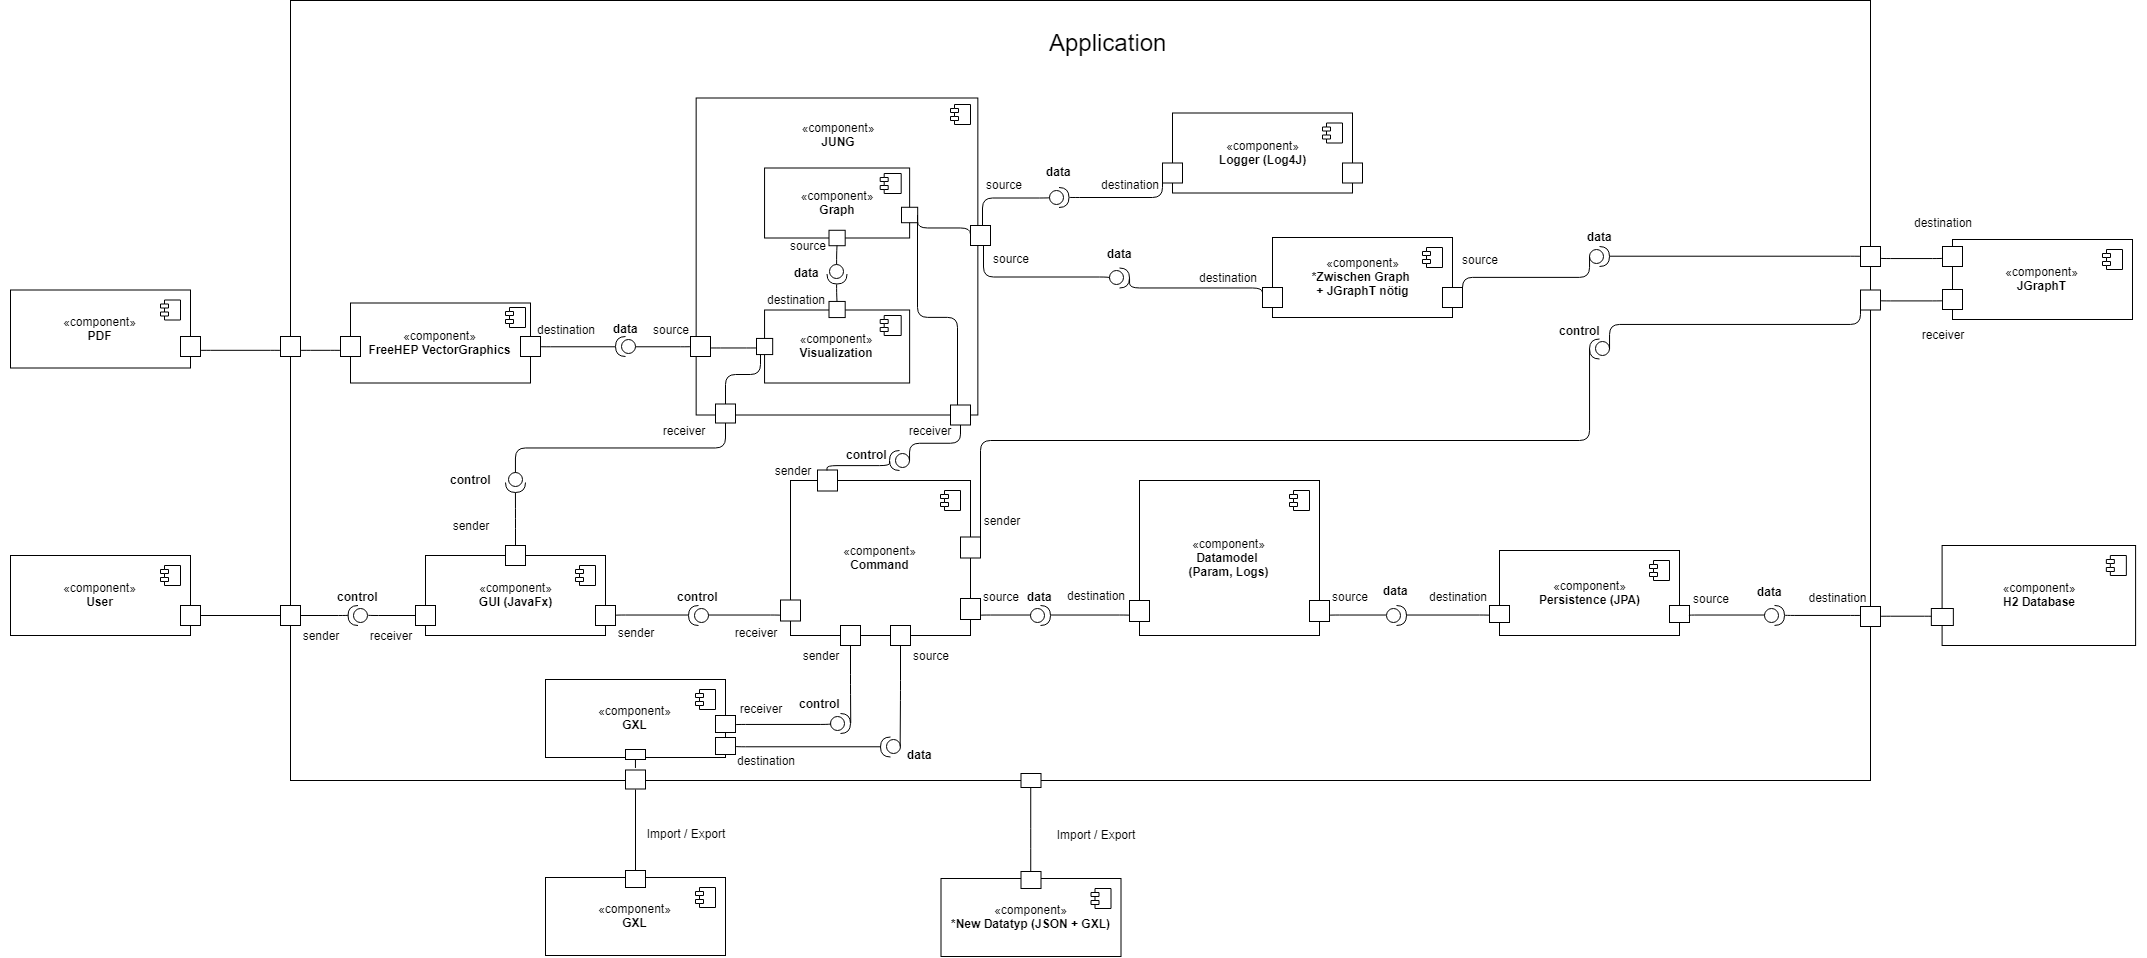
\includegraphics[width=1\textwidth]{KonzeptionelleSicht.png}
	\caption{Konzeptionelle Sicht}
\end{figure}



\newpage
\section{Datensicht}
\label{sec:datensicht}

\emph{Autoren: Anthony Mendil, Clement Phung, Bastian Rexhäuser}\\ \\

Alle Attribute sind private, es existieren aber Getter und Setter (außer bei sämtlichen Id's, dort nur Getter), weshalb sie als public markiert werden. Des weiteren lassen sich die Rollennamen direkt aus den Klassennamen herleiten, weshalb wir sie im Diagramm nicht explizit nennen. (Wir haben uns bezüglich der Klasse \texttt{Vertex} ... keine Ahnung...Hilfe)

\begin{figure}[ht]
\centering
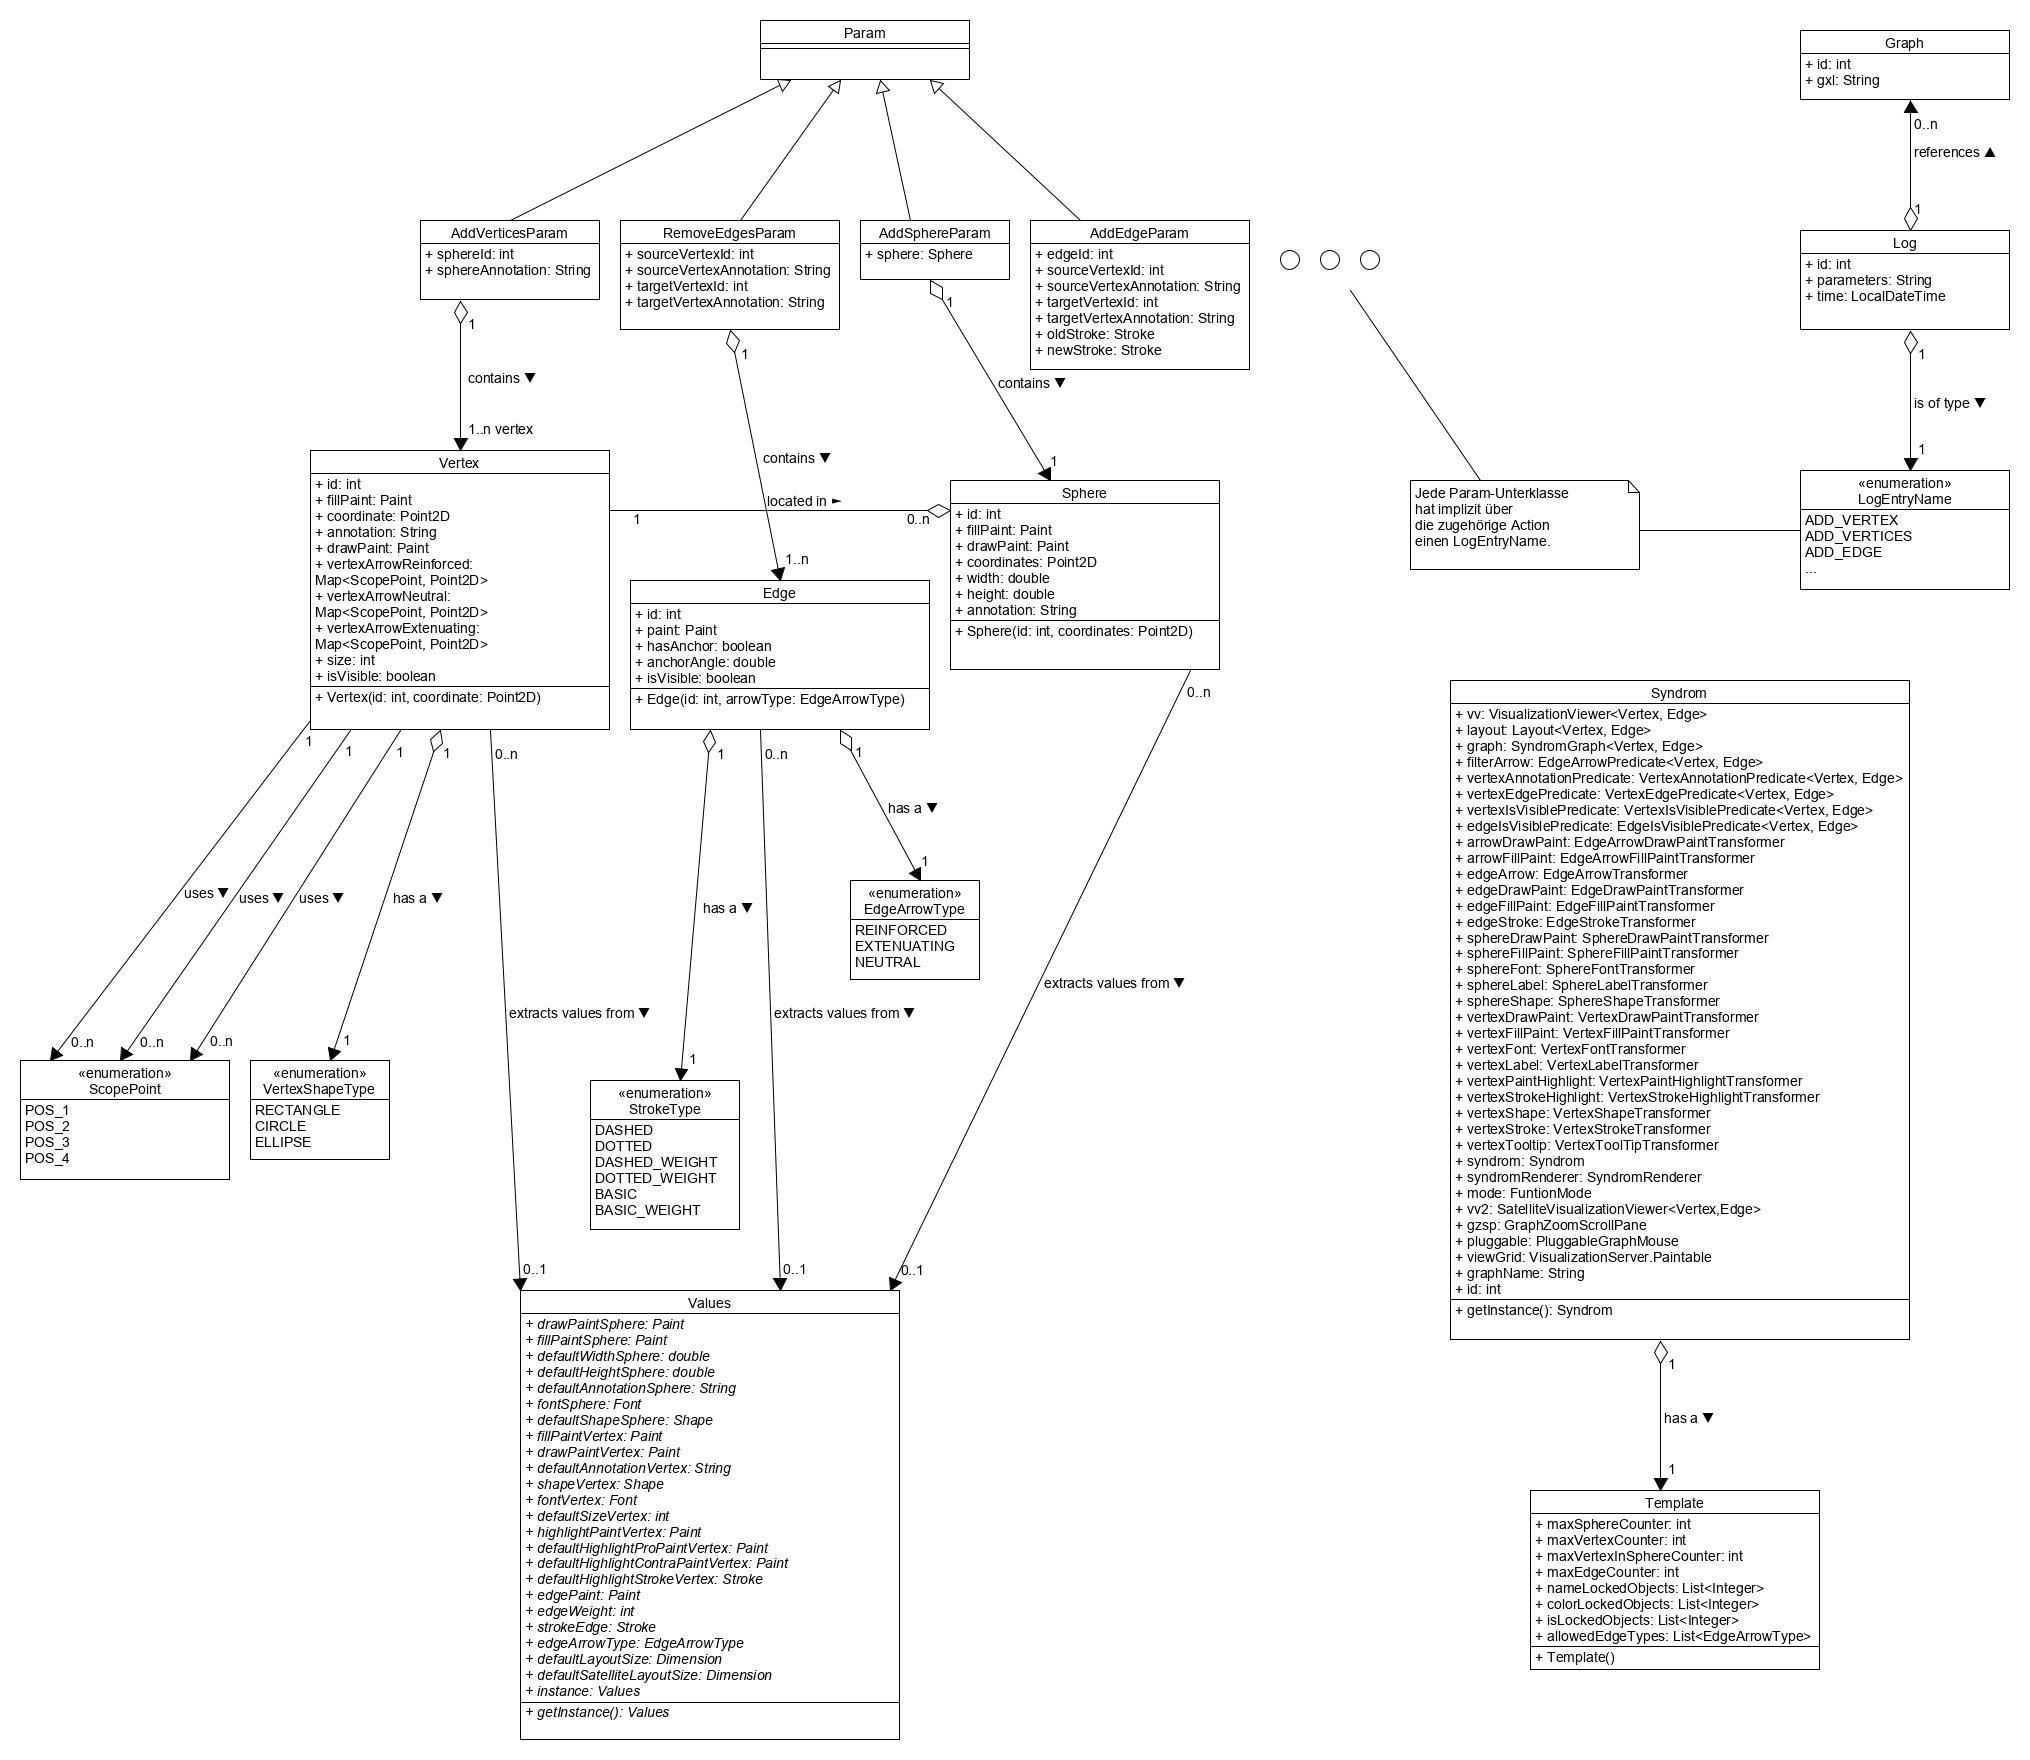
\includegraphics[width=1\textwidth]{Datenmodell_SWP2019.jpg}
\caption{Datensicht}
\end{figure}

\newpage
Im folgenden beschreiben wir unsere Datensicht. Bei Erläuterungen zu dieser beziehen wir uns auf folgende Strategien: \hyperlink{yy}{Strategie S1: GXL}, \hyperlink{aaa}{Strategie S7: Datenmodell}, \hyperlink{eee}{Strategie S19: JUNG}, \hyperlink{jjj}{Strategie 33: JavaScript Object Notation (.json)} und \hyperlink{ooo}{Strategie S43: Eigener Datentyp} sowie auf die \hyperlink{ppp}{Strategie S45: H2 Database}. Außerdem werden wir Bezug zu den Strategien \hyperlink{rrr}{Strategie S.50: Hibernate}, \hyperlink{ttt}{Strategie S56: GXL-Framework (bei Source Forge gehostet)} und \hyperlink{vvv}{Strategie S61: Regeln in der GXL-Datei} nehmen.\\

Es sei an der dieser Stelle explizit angemerkt, dass wir für die Repräsentation des Graphen kein komplett eigenes Datenmodell erstellen. Stattdessen verwenden wir das vom Framework \texttt{JUNG} vorgegebene Datenmodell mit unseren eigenes Datenklassen \texttt{Vertex} (für Knoten) und \texttt{Edge} (für Kanten) (\hyperlink{eee}{Strategie S19: JUNG}). Da in unserem Fall Sphären benötigt werden, erstellen wir eine Klasse \texttt{Sphere} (für Sphären) und erweitern mit ihr das vorgegebene Datenmodell (genauer gesagt erweitert unsere Klasse SydromGraph die Klasse DirectedSparseGraph von \texttt{JUNG}). 
Für die Speicherung des Graphen sowie von allen nötigen Informationen gibt es die Klasse \texttt{Syndrom}. Sie fasst den Graphen, die optionalen Vorgaben/Bearbeitungsregeln (Template) sowie die zum Rendern und zur Visualisierung benötigten Komponenten von \texttt{JUNG} zusammen. \\

Das soeben erwähnte Template ermöglicht es ein Maximum an Sphären, Knoten (im Graphen insgesamt), Knoten in einer Sphäre und Kanten festzulegen. Des weiteren können Objekte des Graphen bestimmt werden, von denen bestimmte Eigenschaften nicht verändert werden dürfen, sowie die Arten der erlaubten Kanten eingeschränkt werden.\\

Die Klasse \texttt{Values} enthält einige Werte, die beim erzeugen eines neuen Graph-Objekts benötigt werden. Es gibt im gesamten Programm nur eine Klasse \texttt{Values} und Nutzeraktionen in der GUI beeinflussen ihre Werte. Setzt der Nutzer beispielsweise die Standardfarbe für neu Symptome um, so wird der entsprechende Wert in der Klasse \texttt{Values} angepasst, sodass neu erzeugte Symptome diese Farbe haben.\\

Um die Persistenz von Daten zu gewährleisten, verwenden wir die embedded Datenbank H2 Database in unserem Programm (\hyperlink{ppp}{Strategie S45: H2}). Bei der Kommunikation mit der Datenbank nutzen wir das Framework Hibernate, welches es unter Verwendung von JPA ermöglicht, Objekte (als Instanzen von Klassen) unseres Systems in eine relationale Datenbank zu persistieren (\hyperlink{rrr}{Strategie S.50: Hibernate}). Hierbei findet ORM (Object-Relational Mapping) Anwendung. \\ 

Um den Graphen zu speichern bietet sich die GXL-Repräsentation (aus den in der Entscheidung für Strategie 1 genannten Gründen) an. Ein als Text-Repräsentation vorliegender Graph wird dabei mit einer Identifikationsnummer versehen und in einer Tabelle unserer Datenbank persistiert. Die Realisierung der genannten Konstruktion lässt sich in der zugehörigen Mapping-Klasse \texttt{Graph} wiederfinden.  Die Übersetzung unseres Graphen in das GXL-Format erfolgt unter Nutzung des bei Sourceforge gehosteten GXL-Frameworks (\hyperlink{ttt}{Strategie S56: GXL-Framework (das bei Source Forge gehostet wird)}). Falls der Benutzer eine Vorlage erstellt, werden auch die darin für die Diagramm-Erstellung im \hyperlink{``Diagramm bearbeiten''-Modus}{``Diagramm bearbeiten''-Modus} gesetzten Einschränkungen in selbiger GXL festgehalten (\hyperlink{vvv}{Strategie S61: Regeln in der GXL-Datei}).\\ 

Die Nutzerinteraktionen mit dem Graphen werden wie auch der Graph selbst in der embedded H2 Datenbank gespeichert. Für die Nutzerinteraktionen existiert eine eigene Tabelle in der Datenbank sowie eine zugehörige Mapping-Klasse \texttt{Log}, welche für jeden Eintrag die relevanten Informationen enthält (\hyperlink{aaa}{Strategie S7: Datenmodell}). Zu diesen Informationen gehört auch ein Text im JSON-Format, der aus dem jeweiligen Parameterobjekt erzeugt wird (\hyperlink{jjj}{Strategie 33: JavaScript Object Notation (.json)}). Es sei explizit erwähnt, dass zu einem Log ein Graph gehört, der Graph dennoch nichts vom Log weiß und von diesem auch keine Informationen lesen kann. Die bereits erwähnten Parameterklassen sind Unterklassen der Klasse \texttt{Param} und implementieren alle eine Methode, die den zugehörigen String im JSON-Format erzeugt. Jede dieser Parameter-Klassen gehört speziell zu einer Aktion, für die sie die nötigen Informationen enthält. Es ist hierbei anzumerken, dass die einzelnen Parameter-Klassen im Diagramm individuell Assoziationen  (manche auch keine) zu den Klassen \texttt{Vertex}, \texttt{Edge} und \texttt{Sphere} hätten, je nachdem welche Attribute sie besitzen. Um Übersichtlichkeit zu bewahren haben wir im Diagramm nicht alle Parameter-Klassen mit ihren zugehörigen Attributen dargestellt, sondern exemplarisch vier solcher Klassen ausgewählt. Alle Parameter-Klassen lassen sich im Package \texttt{log\_management.parameters finden}. \\

In unserem Programm ist ebenfalls das Exportieren einzelner Graphen mit den zugehörigen Log-Einträgen möglich. Dies geschieht anhand eines selbst entwickelten Dateiformates (oof für \glqq out of frameworks\grqq). (\hyperlink{Strategie S43: eigener Datentyp}{Strategie S43: eigener Datentyp})


\newpage
\section{Modulsicht}
\emph{Autoren: Anthony Mendil, Bastian Rexhäuser, Clement Phung, Jacky Philipp Mach, Jonah Jaeger, Nina Unterberg}\\\\

In folgenden ist der statische Aufbau unseres Systems in Form der Modulsicht zu finden. In dieser werden besonders wichtige oder für eine Gruppe von Modulen stellvertretend stehende Module unseres Systems genannt. Dabei wird auf die Funktion und Notwendigkeit dieser Module eingegangen sowie teilweise deren grundlegender Aufbau thematisiert. Außerdem wird in diesem Kapitel beschrieben wie die Module zusammenwirken, um die geforderten Anforderungen zu erfüllen. Bei Ausführungen zur Bedeutung, zum Aufbau und zum Zusammenwirken von Modulen wird bezug zu den Strategien genommen, für die wir uns im Rahmen der Problemkarten im Kapitel „Globalen Analyse“ entschieden haben. \\ \\

\newpage

\subsection{Übersicht}
Dieser Abschnitt beschäftigt sich mit einer Übersicht über alle Module des gesamten Projektes. \\
Die Zusammenhänge zwischen den Modulen wurde auf der folgenden Seite als Paketdiagramm dargestellt.
Im Allgemeinen ist die Struktur des Projektes angelehnt an das Model-View-Controller-Designpattern, gemäß der Strategie “\hyperlink{bbb}{S8 - MVC}”. Das Package \texttt{gui} setzt die View um, \texttt{log\_management} die Model Komponente und \texttt{actions} die Controller Komponente. \\

Das Package \texttt{actions} beinhaltet \texttt{Action} Klassen, die vor allem Aktionen auf dem Graphen umsetzen. Diese \texttt{Action} Klassen werden mit der Interaktion der grafischen Benutzeroberfläche verknüpft, sodass z.B. bei Klick auf einem Button eine bestimmt Aktion ausgeführt wird. \\

Das Modul \texttt{gui} beinhaltet alle Klassen, die zur Erstellung/ Interaktion mit der Benutzeroberfläche benötigt werden. Die \texttt{GUI} steht in Abhängigkeit mit dem Modul \texttt{actions}, da die \texttt{Actions} mit den Interaktionen auf der \texttt{GUI} verknüpft sind. Die \texttt{GUI} bezieht sich außerdem auf das Modul \texttt{log\_management}, da diese im Modus \textit{Analyse} Informationen über das Protokoll visualisiert. Im Modus \textit{Vorlage bearbeiten} und \textit{Diagramm bearbeiten} werden Informationen über den Graphen visualisiert, weshalb hier ebenfalls eine Abhängigkeit zu dem package \textit{graph} besteht. \\

Das Persistieren der Daten wird im Package \texttt{log\_management} umgesetzt. Dieses Package ist in drei weitere Packages unterteilt: \texttt{dao}, \texttt{parameters} und \texttt{tables}. \texttt{dao} ''Data Acess Object'' bildet die Benutzerschnittstelle für die anderen Module, um auf die Daten in der Datenbank zuzugreifen. Das Package \texttt{parameters} beinhaltet \texttt{Param} Klassen. Jeder \texttt{Action} Klasse ist eine \texttt{Param} Klasse zugeordnet. Diese wird bei der Persistierung der \texttt{Actions} als \texttt{Log} in einen Json-String umgewandelt und als Attribut eines \texttt{Log} Objektes abgespeichert und in die Datenbank geschrieben. \texttt{tables} beinhaltet die Klassen, welche den Aufbau eines \texttt{Graph}- und \texttt{Log} Objektes beschreiben. Diese Objekte werden mit Hibernate/ JPA persistiert und in einer embedded H2DB abgespeichert. \\ 

Alle Import und Export Aktionen, werden im Package \texttt{io} implementiert. \texttt{io} benötigt die Protokoll Daten, welche durch das Package \texttt{dao} zugänglich sind. Außerdem greift \texttt{io} auf Klassen aus \texttt{graph} zu, da dort die Klassen liegen, welche die Daten zu dem aktuellen \textit{Syndromansatz} beinhalten. \\

Das Package \texttt{jgrapht} setzt die Funktionalität um, einen Graphen aus unserem System in einen Graphen umzuwandeln, der vom Framework jgrapht erkannt wird. Deswegen besteht eine Abhängigkeit zwischen dem Package \texttt{jgrapht} und \texttt{graph.graph}. \\

Alle Klassen, die Funktionalität für den Programm internen Graphen umsetzen, sind im Package \texttt{graph} implementiert.  Dieses Package ist in drei Packages unterteilt: \texttt{algorithm}, \texttt{graph} und \texttt{visualisation}. \texttt{algoithm} beinhaltet Klassen, die unseren Graphen nach bestimmten Bedingungen/ Algorithmen filtern. \texttt{graph} beinhaltet alle Datenklassen zu dem Graphen und Funktionalitäten, die benötigt werden, um den Graphen umzusetzen. \texttt{visualization} stellt Klassen zur Verfügung, die die visuellen Eigenschaften des Graphen bestimmen und darstellen. \\

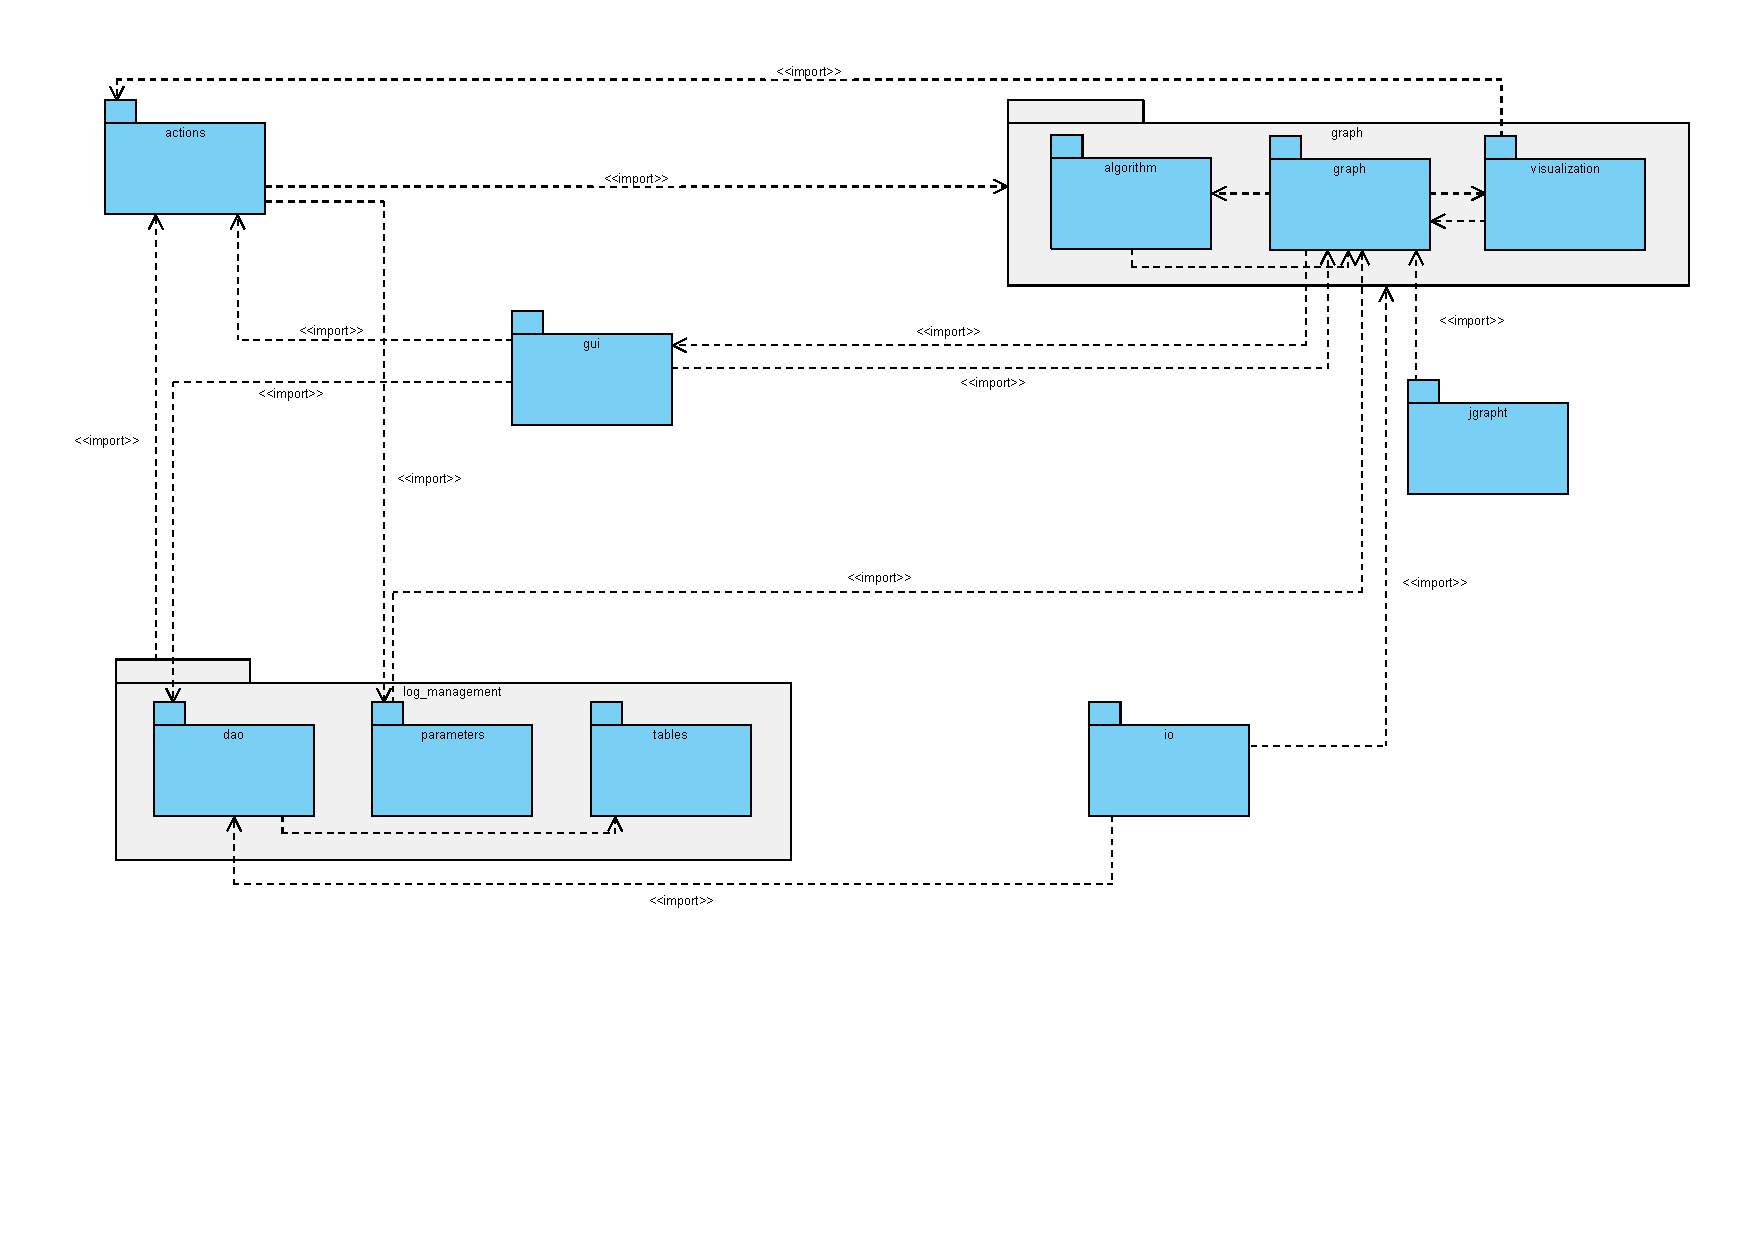
\includepdf[pages=-, landscape, scale=0.84,pagecommand={\pagestyle{fancy}}]{package.pdf}

\subsection{\texttt{io}}
Der Graph soll gemäß Strategie \hyperlink{yy}{S1 – GXL} "'plain"' als String in der Datenbank abgespeichert werden. Dieser String beinhaltet eine GXL (Graph eXchange Language) –Repräsentation des Graphen.\\
Daher muss es ein Modul geben, welches alle Informationen des in der GUI angezeigten Graphen abfragt und diesen in ein GXL-Format transferiert. Analog dazu muss die Möglichkeit bestehen, aus einem GXL-String die \texttt{Syndrom}-Instanz beziehungsweise Graph-Repräsentation zu generieren, die dann als aktueller Graph im Programm angezeigt wird.\\ 

Außerdem soll das Programm die Möglichkeit bieten, eine GXL Datei zu importieren/exportieren. Diese Funktionalität muss gemäß Einflussfaktor \hyperlink{ii}{GXL- Export und -Import} bereit gestellt werden.\\ 
Für die Umsetzung dieser Funktionen haben wir im \texttt{io-package} die Klasse \texttt{GXLio} implementiert. \\

In der Klasse \texttt{GXLio} sind io-Methoden für die GXL-Repräsentation des Graphen zu finden, welche (neben dem Dateinamen beim Import) den Pfad der zu importierenden Datei beziehungsweise den Pfad für die zu exportierende Datei übergeben bekommen (\texttt{importGXL(), exportGXL()}). \\
Um die Funktion vollständig zu realisieren sind außerdem je eine Methode zum Schreiben der GXL-Daten in die \texttt{Syndrom}-Instanz (\texttt{gxlToInstance()}) sowie zur Erstellung einer GXL-Repräsentation aus der Instanz (\texttt{gxlFromInstance()}) vorgesehen. \\
Zweitere Methode ist außerdem für die genannte GXL-Speicherung in der Datenbank nützlich, da sie genau die benötigte GXL-Variante des Graphen bereitstellt.\\ 

Über die injizierten Instanzen der \texttt{Syndrom}- und \texttt{GraphDao} Klasse, erhalten die Objekte der \texttt{GXLio} Klasse alle Informationen zu dem in der \texttt{GUI} visualisierten Graphen. \\
Um diese Informationen in das GXL-Format zu überführen, wird im Zuge der Implementierung das GXL-Framework von SourceForge verwendet (siehe Strategie \hyperlink{xaa}{S56 Sourceforge Framework}).\\

Durch das \texttt{Template-Attribut} in der \texttt{Syndrom} Klasse haben Methoden, welche eine GXL-Repräsentation eines Graphen erstellen, aus einem \texttt{Syndrom} Objekt auch Zugriff auf die Bearbeitungsregeln, denn diese werden in einem Objekt der \texttt{Template} Klasse hinterlegt.
Durch diesen Ansatz können die Bearbeitungsregeln in einer GXL-Repräsentation gespeichert werden, gemäß der Strategie \hyperlink{vvv}{S61 - Regeln in der GXL-Datei}. \\ 

Da wir nicht nur den Graphen isoliert als GXL-Datei exportieren, sondern ihn auch zusammen mit den Nutzerinteraktionen als OOF-Repräsentation bereitstellen wollen, haben wir die Klasse \texttt{OOFio} hinzugefügt. Diese ist ebenfalls im \texttt{io} Package zu finden. Mit dieser wollen wir die gemeinsame Speicherung der Nutzerinteraktionen mit einem (als GXL-Repräsentation vorliegendem) Graphen realisieren (Startegie \hyperlink{ooo}{S43 - Eigener Datentyp}). \\

Um diesen gemeinsamen Datentyp zu erzeugen, gibt es die Methode \texttt{createOOF()}, die eine GXL-Repräsentation eines Graphen und Nutzerinteraktionen als JSON erhält, wobei diese beiden Parameter je als String übergeben werden. Diese Methode wird benötigt, um die übergebenen Werte zusammenzuführen und zu exportieren. \\
(\texttt{exportOOF()}) speichert die zusammengeführten Informationen als Datei eines eigenen Datentyps (im \texttt{.oof}-Format), an dem Pfad und mit dem Namen der Datei, den die Methode übergeben bekommt. \\

Diese Datei muss jedoch auch wieder geöffnet werden können. Dies geschieht durch die Methode \texttt{importOOF()}. Diese bekommt den Pfad der zu importierenden Datei als String und schreibt die Daten in die Datenbank (Protokoll) und in die Instanz (Graph). Dabei benutzt sie die Methoden \texttt{gxlFromOOF()} und \texttt{jsonFromOOF()}, welche jeweils die OOF-Datei als String bekommen und die jeweiligen Datenteile zurückgeben. \\
Da die \texttt{OOFio}-Klasse zur Erstellung einer .oof-Datei ein GXL-String benötigt, wird ein Objekt vom Typ \texttt{GXLio} erstellt und auf diesem die Methode \texttt{gxlFromInstance()} aufgerufen.\\ 

Damit die Klasse die genannten Funktionalitäten umsetzen kann, bekommt sie das \texttt{LogDao}- und \texttt{GraphDao}-Objekt injiziert. 

Mit den Methoden der \texttt{PDFio}-Klasse aus dem \texttt{io-package} sind unter Einsatz der Frameworks, beziehungsweise APIs, der PDF-Druck (gemäß Strategie \hyperlink{ggg}{S26: Java API}) und der PDF-Export (gemäß Strategie \hyperlink{iii}{S30 - Freeheb Vectorgraphics}) realisierbar. \\
Der Aufruf zum Drucken geschieht durch \texttt{printPDF()}, während der Export als PDF in \texttt{exportPDF()} implementiert wird. Für diese Methoden ist die Methode zur PDF-Erstellung (gemäß Strategie \hyperlink{hhh}{S29 - java.awt.Graphics2D} nützlich. Diese ist als \texttt{createPDF()} implementiert und gibt die PDF als Datenstrom wieder. \\
\texttt{PDFio} bekommt im \texttt{constructur} den \texttt{VisualizationViewer} des angezeigten Graphen übergeben, um die PDF zu erstellen.

\newpage
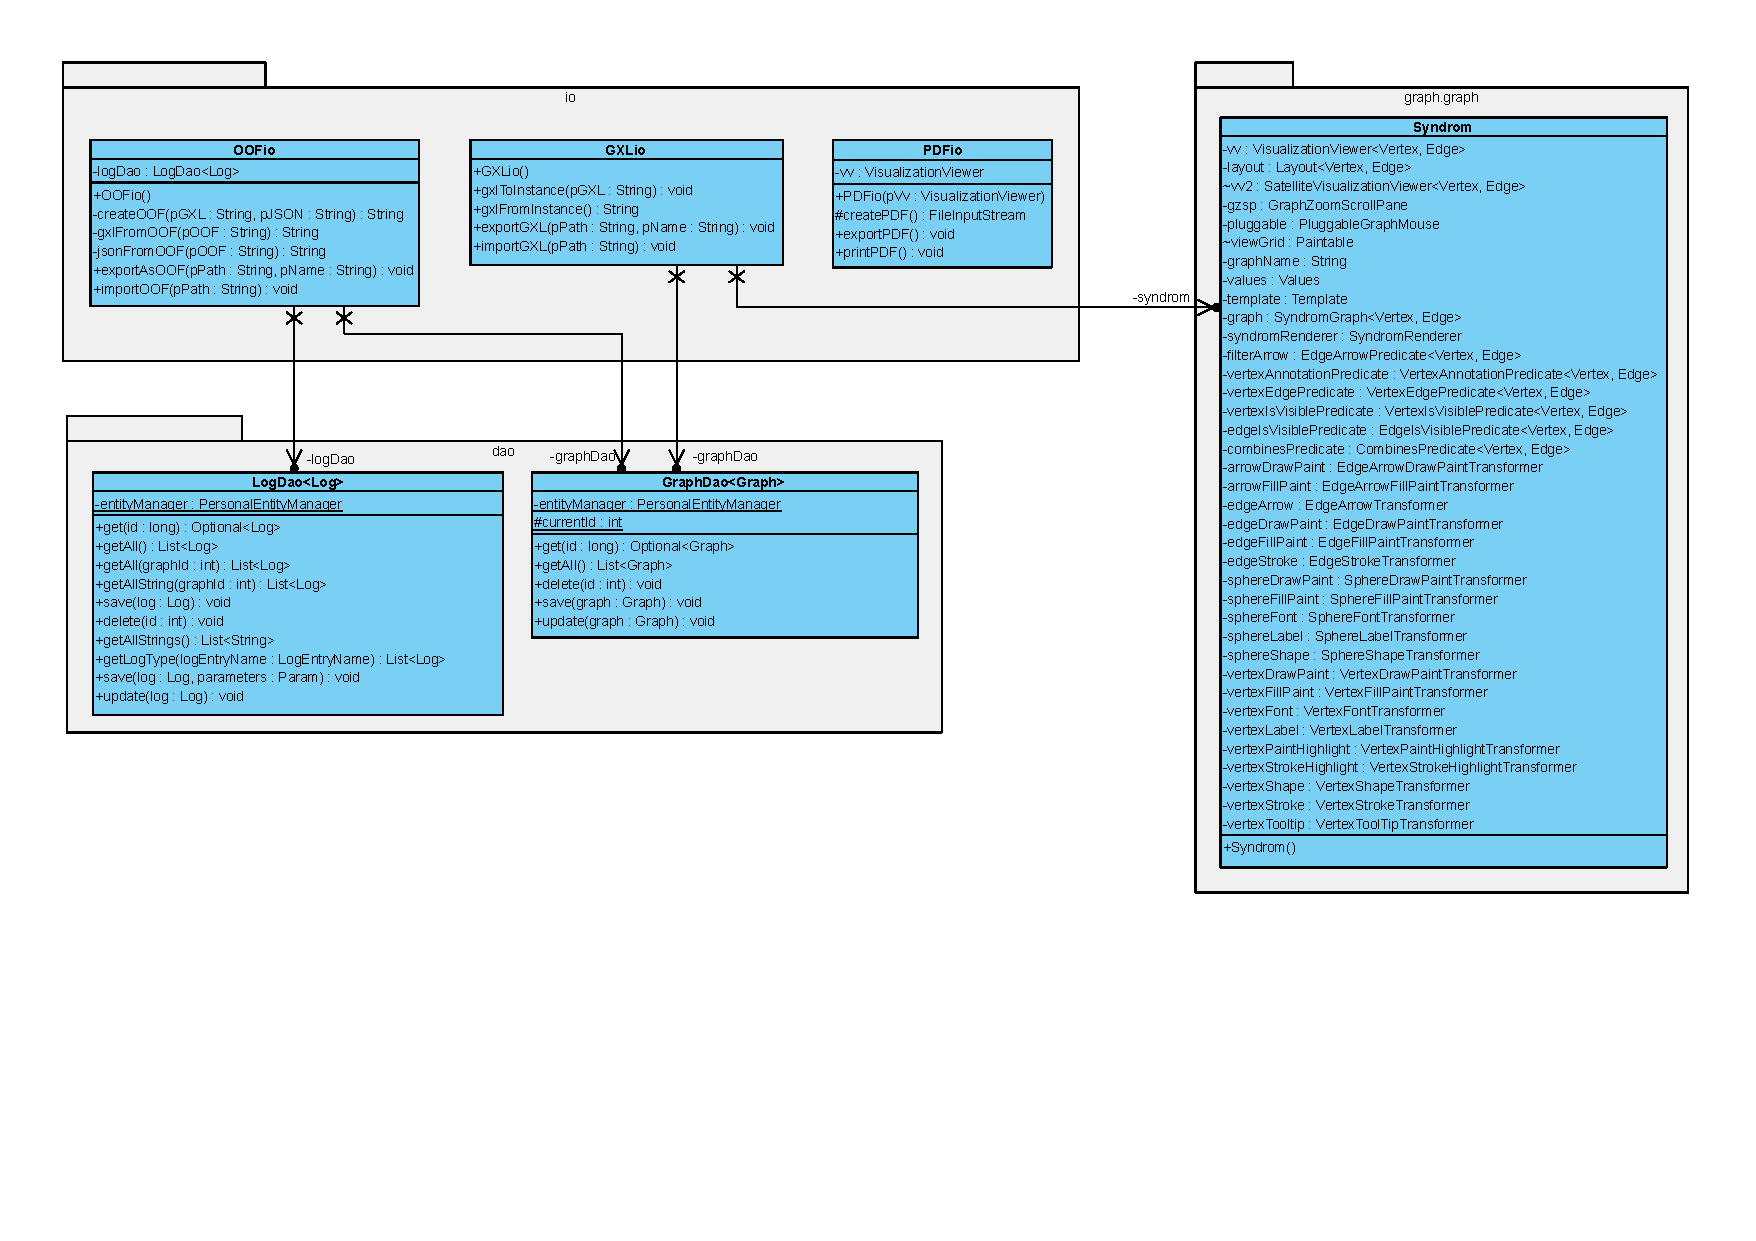
\includepdf[pages=-, landscape, scale=0.84,pagecommand={\pagestyle{fancy}}]{io.pdf}


\subsection{\texttt{gui}}
Die Benutzeroberfläche wurde mit JavaFx (siehe Strategie \hyperlink{kkk}{S34 - GUI Framework JavaFx}) und mit Hilfe der Anwendung \textit{SceneBuilder} von Gluon, gemäß der Strategie \hyperlink{mmm}{S38 - Scene-Builder}, umgesetzt. Die erstellte \texttt{GUI} ist in der Applikation als FXML-Datei gespeichert und wird beim Starten unserer Applikation in der \texttt{Main}-Klasse geladen. Sie ist außerdem auch zuständig für das Starten der gesamten Anwendung. \\

Um die GUI mit der gewünschten Funktionalität der Applikation zu verbinden, existiert die Klasse \texttt{Controller}. Sie dient als Schnittstelle zwischen der \texttt{GUI} und den internen Modulen. \\
FXML ist sehr gut geeignet, um die Darstellung der \texttt{GUI} Elemente zu definieren und die Methoden in \texttt{Controller} jeweils zu den Elementen zu zuordnen. Diese Methoden werden beim Interagieren mit den \texttt{GUI} Elementen aufgerufen und müssen in der Controller Klasse angegeben werden. Da einige \texttt{GUI} Elemente jedoch mehr Funktionalität benötigen als nur ein Methodenaufruf beim Interagieren, werden diese Element nochmals referenziert in der \texttt{Controller} Klasse um sie zu erweitern.\\

Die \texttt{Controller}-Klasse besitzt außerdem die internen Klassen \texttt{ColorPickerHandler} und \\ \texttt{MenuItemHandler}. Diese werden benötigt, da die \texttt{GUI} Elemente \texttt{MenuItem} und \texttt{ColorPicker} zusätzlich an die aufgerufene Methode übergeben müssen, welchen Wert der User ausgewählt hat, beispielsweise die gewählte Farbe. \\
Diese Werte werden zusätzlich in dem Singleton Objekt der Klasse \texttt{Values} den zugehörigen Attributen zugewiesen, damit die \texttt{Actions} Objekte und das \texttt{Syndrom} Objekt auf diese Werte zugreifen können. \\

Zur Graph Visualisierung wird das Framework \hyperlink{eee}{JUNG} verwendet. Da dieses Framework auf Swing basiert, wird die Swing-Komponente, in die mit JavaFX erstellte GUI, durch eine Swing-Node eingebunden. Dieses Vorgehen folgt Strategie \hyperlink{lll}{S36 - SwingNode}.\\

Da die \texttt{GUI} den Graphen außerdem in der Seitenleisten in textueller, strukturierter Form darstellen soll, benötigt die \texttt{GUI} Informationen über die Objekte des Graphen. Die Information sind über das \texttt{Syndrom} Objekt aus dem Package \texttt{graph.graph} zugänglich. \\

Das Objekt der Klasse \texttt{ActionHistory} aus dem Package \texttt{actions} wird benötigt, um die \hyperlink{command}{Actions} mit den Interaktionen des Users zu verknüpfen. Diese führt zuvor erstelle Actions aus. Außerdem kann so die benötigte \texttt{redo} und \texttt{undo} Funktionalität umgesetzt werden. \\

Das Interface \texttt{ObserverSyndrom} aus dem Package \texttt{actions} wird implementiert, um die Veränderungen des Graphen auf der GUI zu updaten.\\

Um das Anzeigen des Protokolls der Nutzerinteraktion zu ermöglichen, bekommt die \texttt{Controller}-Klasse das Benutzerprotokoll über ein Objekt der \texttt{LogDao}-Klasse aus dem Package \texttt{dao}. Dieses bildet die Schnittstelle zur Datenbank. \\

Die Klasse \texttt{LoadLanguage} besitzt noch weitere GUI-Elemente zusätzlich zu den bereits referenzierten in der \texttt{Controller-Klasse}, um die Texte der \texttt{GUI} bei Bedarf auf eine andere \hyperlink{hh}{Sprache} umzustellen.
	

\newpage
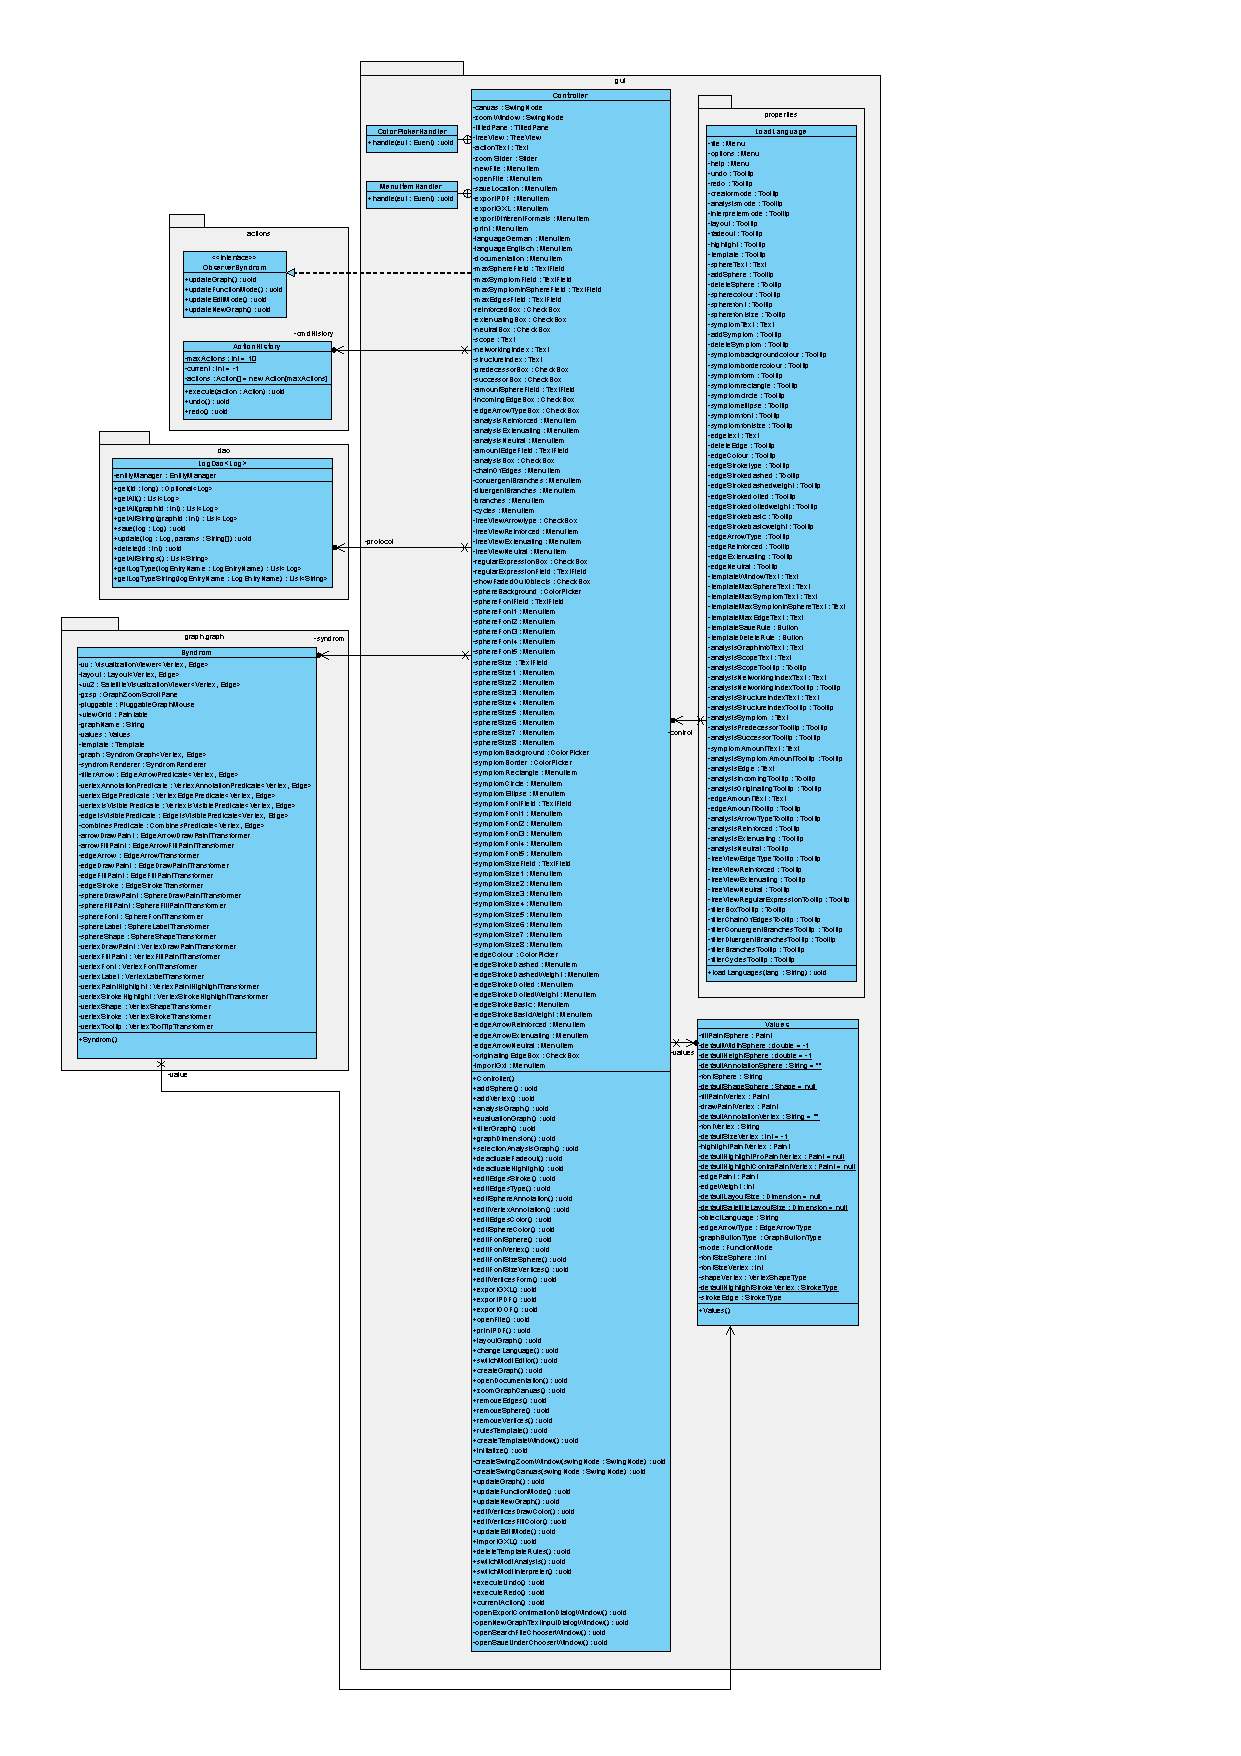
\includepdf[pages=-, scale=0.84,pagecommand={\pagestyle{fancy}}]{gui.pdf}



\subsection{\texttt{actions}}
Das Package \texttt{actions} repräsentiert die Controller Komponente des Model-View-Controller Patterns, welches wir gemäß \hyperlink{bbb}{S8- MVC} umsetzen. \\ 
Diese ist nach dem \texttt{Command} Pattern nach \hyperlink{command}{S9 - Command} aufgebaut. \\

Die abstrakte Klasse \texttt{Action} stellt die Oberklasse dar. Diese implementiert zwei abstrakte Methoden \texttt{redo}/ \texttt{undo}. Eine weitere abstrakte Klasse \texttt{GraphAction} erweitert die \texttt{Action}-Klasse. Jede \texttt{GraphAction} wird ein \texttt{Syndrom} injected. Durch dieses \texttt{Syndrom} Objekt verfügt jede \texttt{GraphAction} über die benötigten Informationen zu dem visualisierten Graphen. Da \texttt{Syndrom} ein Singleton ist, verfügt nach einer Änderung des Graphen das ganze System darüber und kann es entsprechend visualisieren.  Dies ist erforderlich, damit sich die vom Nutzer durchgeführten Aktionen auch auf den gerade in Bearbeitung befindlichen Graphen auswirken.\\ 
Eine weitere abstrakte Klasse setzt die benötigte Funktionalität für eine \texttt{LogAction}. Zudem haben alle \texttt{LogActions} eine Verbindung zu \texttt{LogEntryName} und zu \texttt{Param}. Dies ist beides für die Persistierung von Bedeutung. Die Verbindung zu \texttt{Param} bedeutet, dass zu jeder \texttt{LogAction} ein Objekt einer konkreten Unterklasse der abstrakten Oberklasse \texttt{Param} gehört. \\
Diese Parameterobjekte werden erzeugt, wenn eine Aktion ausgeführt wird und beinhalten die Parameterdaten der Action. So ist es möglich, zu jedem Zeitpunkt die genauen Daten aller \texttt{LogActions} auszulesen (da diese ja in die Datenbank persistiert werden). Dies hilft bei der Umsetzung der \texttt{undo}- und \texttt{redo}-Funktion. Die Actions sind unsere Umsetzung der Strategie \hyperlink{xcc}{S9 - Command}  \\


Wie man aufgrund der Existenz der Klasse \texttt{SwitchModiEditorAction} im \texttt{actions.other}Package bereits erahnen kann, wird das Umschalten zwischen den Fuktionsmodi ebenfalls über eine Action realisiert. Der aktuelle Funktionsmodus wird dabei in der Klasse \texttt{Values} im Package \texttt{gui} gespeichert.  Die Funktionsmodi, die in unserer Anwendung existieren, sind in der Enum \texttt{FunctionMode} im \texttt{graph.graph} Package zu finden. Die beschriebene Umsetzung folgt der Strategie \hyperlink{uuu}{S59 - Modi als eigener Teil unserer Applikation}.
\texttt{AnalysesGraphAction} steht mit \texttt{AnalyseTypeSingle} und mit \texttt{AnalyseTypeSeveral} aus dem Package \texttt{graph.algorithmen} in Abhängigkeit, um den oder die ausgewählten Filteroptionen ausmachen zu können, die von der Analyse betroffen sein sollen. \\\\

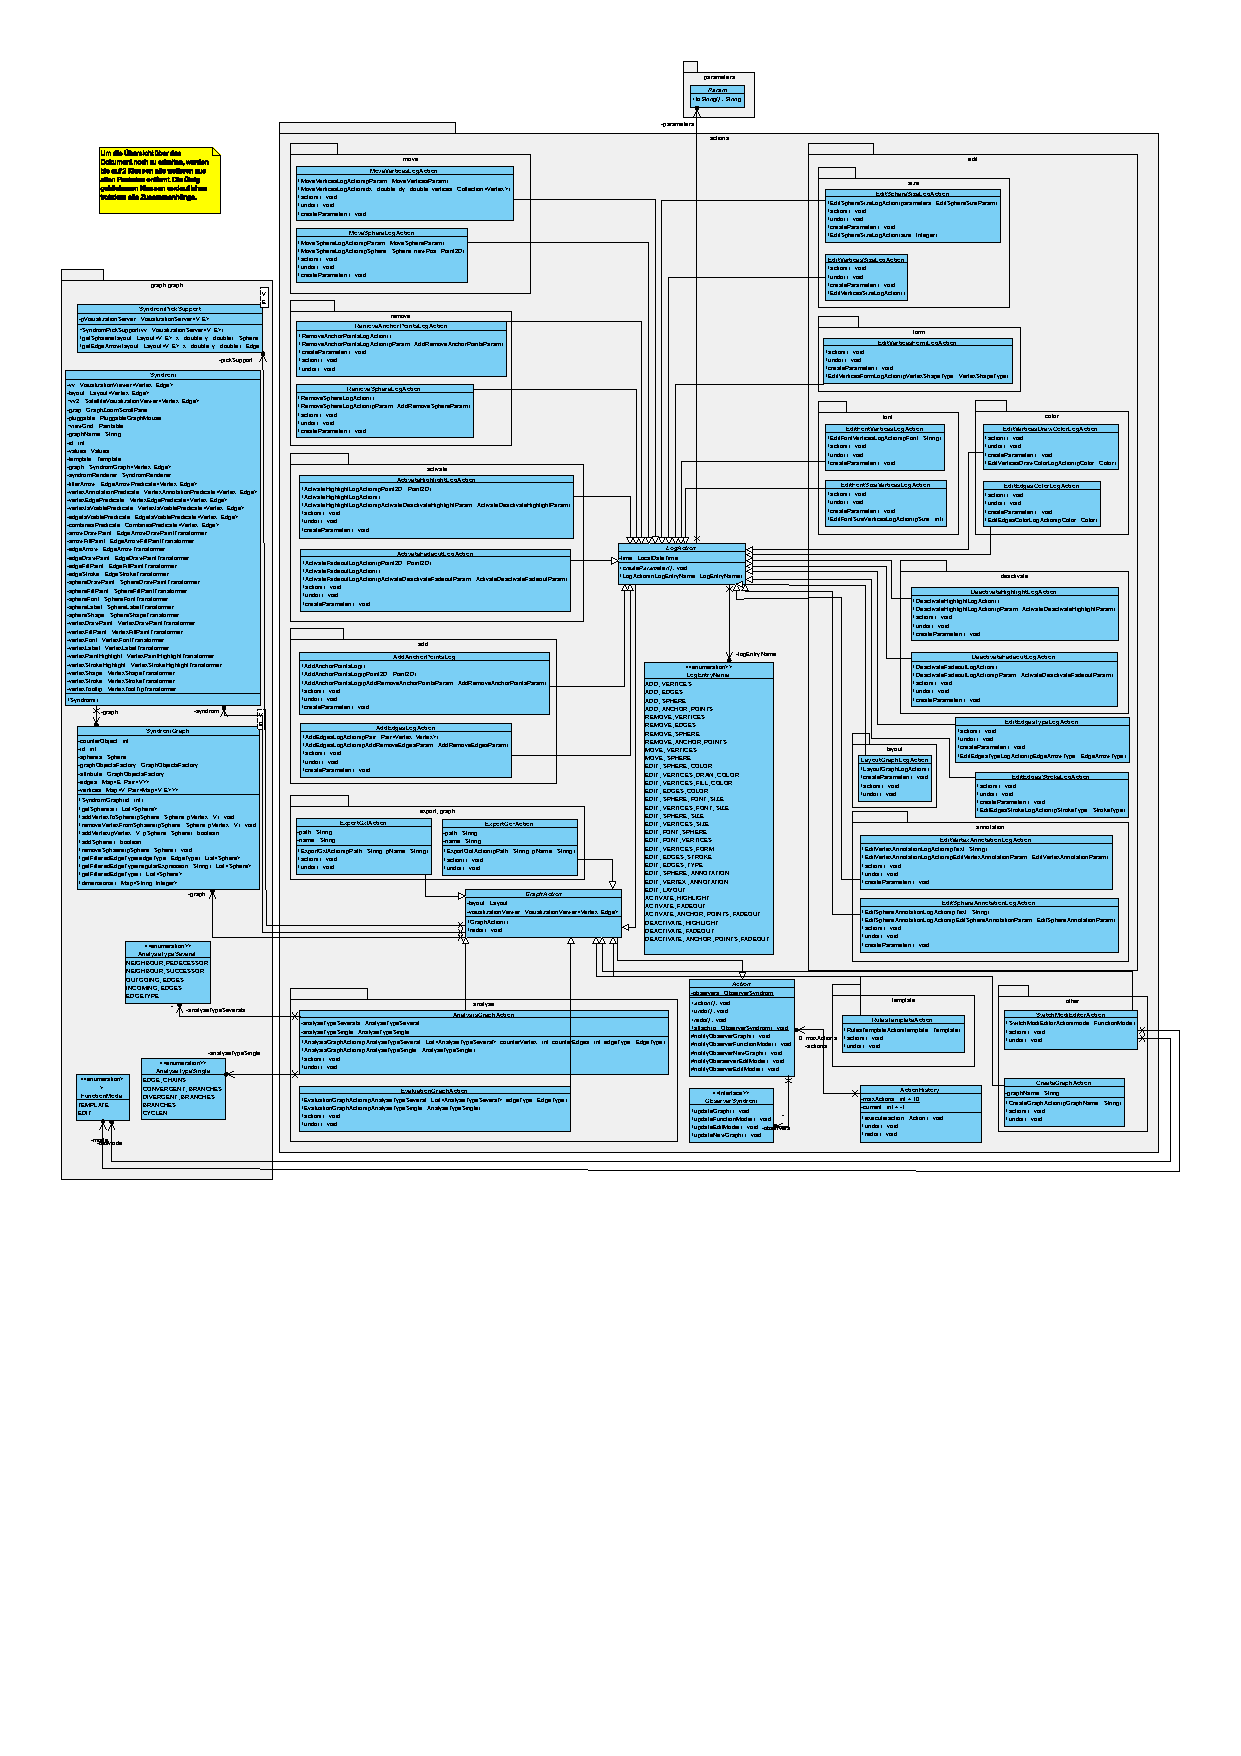
\includepdf[pages=-, scale=0.84,pagecommand={\pagestyle{fancy}}]{actions.pdf}

Eine Übersicht über alle \texttt{Action} packages, die der Übersicht halber auf der vorherigen Abbildung nicht komplett dargestellt werden konnten, werden auf der folgenden visualisiert. 

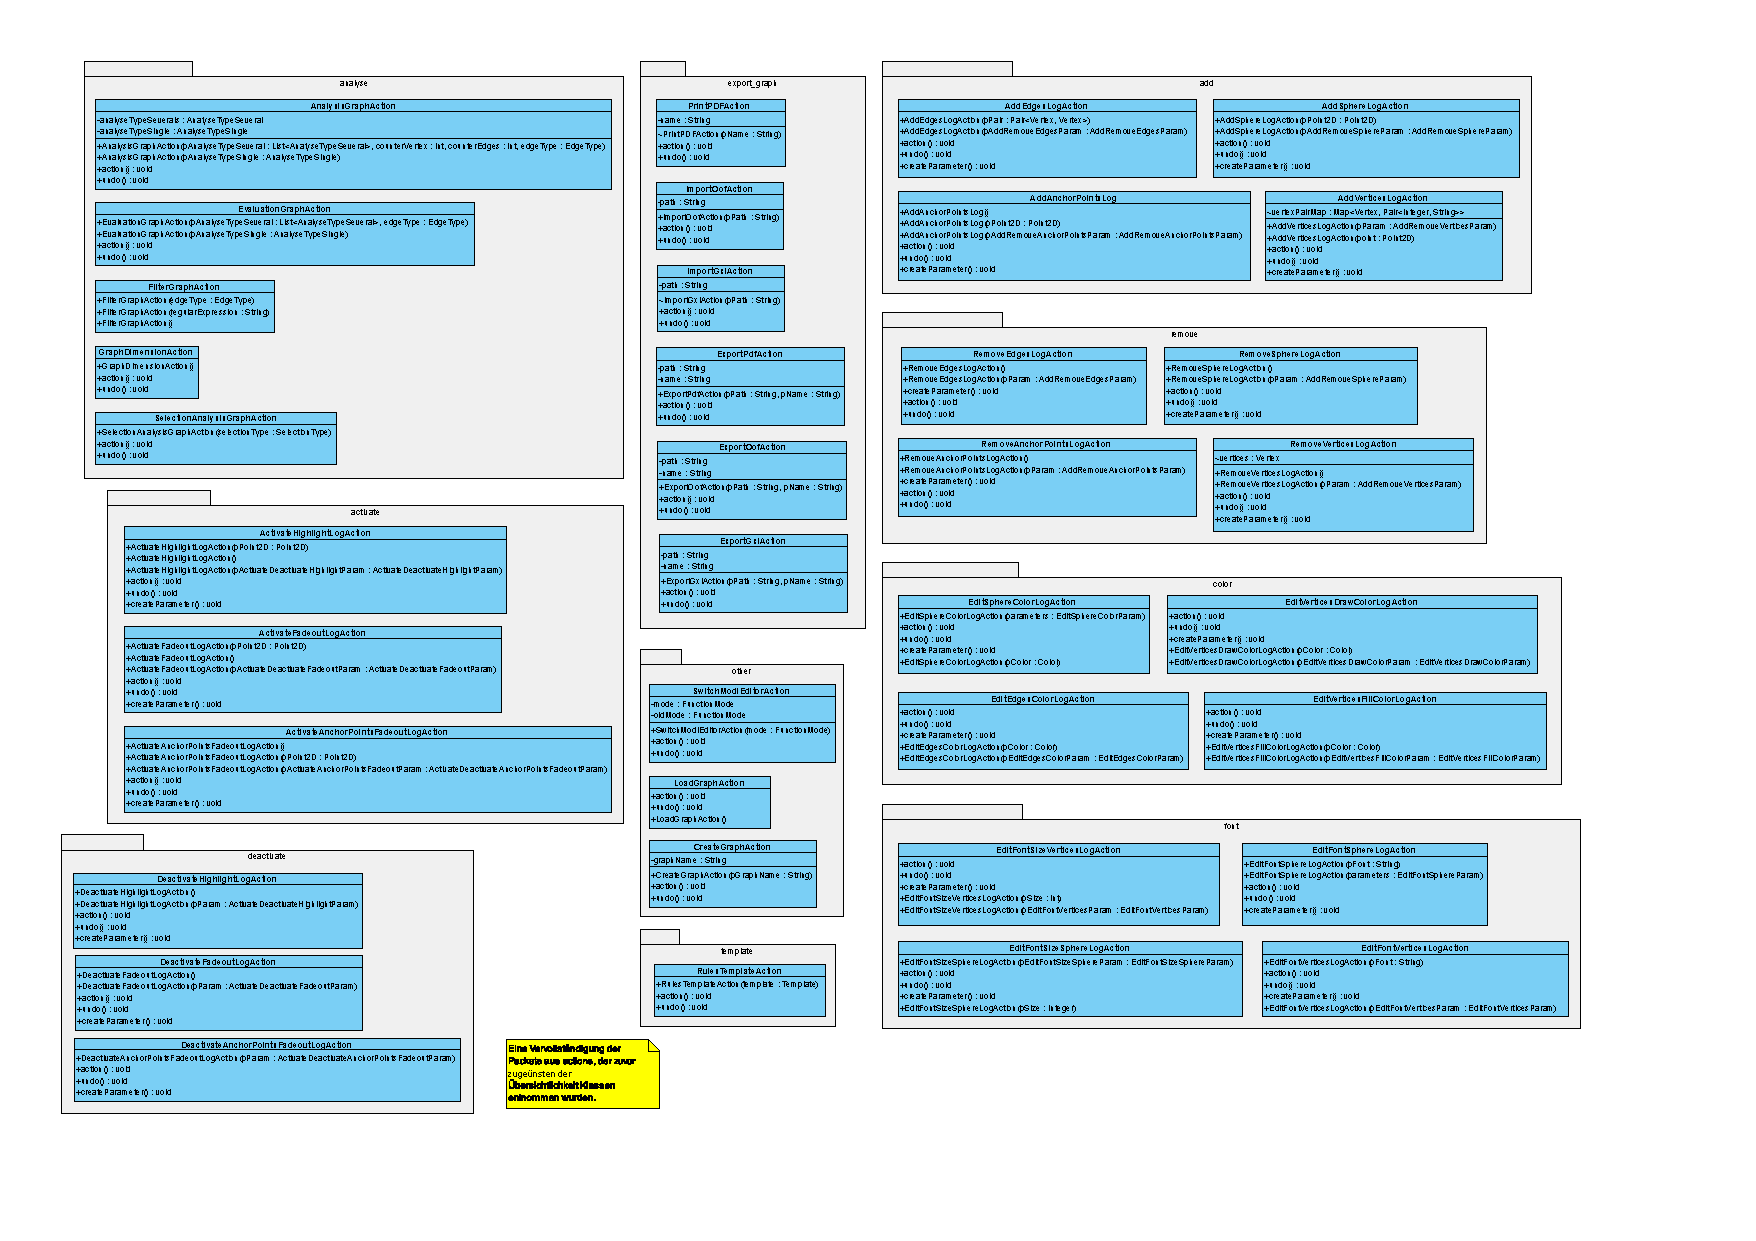
\includepdf[pages=-, scale=0.84,pagecommand={\pagestyle{fancy}}]{actionsOverview.pdf}


\subsection{\texttt{log\_management}}

Die Umsetzung der Strategie \hyperlink{aaa}{S7 - Datenmodell} ist in der Klasse \texttt{Log} im Package \texttt{log\_management/tables} zu sehen. Im Package \texttt{log\_management} werden neben der Speicherung der Nutzerinteraktionen in Form der Logs die weiteren Aspekte der Persistierung umgesetzt. \\
Die Daten -Persistierung setzen wir mit Hilfe von \hyperlink{rrr}{S50 - Hibernate} um. Die im Package \texttt{tables} liegende Klassen stellen die Objekte dar, die wir in der Datenbank persistieren wollen. 



Dabei sind die \texttt{Log} Objekte wie beschrieben zur Speicherung der Nutzerinteraktionen erforderlich, während die \texttt{Graph} Objekte eine \hypertarget{yy}{Graphrepräsentation} beinhalten. \\

Die \texttt{Log} Objekte besitzen unter anderem ein Attribut \texttt{parameters}. Dieses Attribut repräsentiert ein zugehöriges \texttt{Param} Objekt als String. Die \texttt{Param} Objekte beinhalten alle wichtigen Informationen zu der zugehörigen Aktion, damit diese verständlich für den Benutzer rekonstruiert werden kann. Dieser String wird durch eine Konvertierung eines \texttt{Param} Objektes zu einem \texttt{JSON} String erzeugt. Die \texttt{JSON}- Umwandlung erfolgt gemäß \hyperlink{www}{S63- Jackson} mit Jackson. \\

Die \texttt{Graph} Objekte haben ein Attribute \texttt{gxl}, welches den visualisierten Graphen als GXL- Repräsentation gemäß \hyperlink{yy}{S1 - GXL} beinhaltet. Der GXL- String wird durch das \texttt{io} Package realisiert, weshalb hier auch eine Abhängigkeit besteht.\\

Die Existenz des Package \texttt{parameters} sorgt dafür, dass die Nutzerinteraktionen in den Logs beschrieben werden können. Daneben gehört zu jedem \texttt{Log}-Eintrag unter anderem ein \texttt{Graph} und ein \texttt{LogEntryName} - wie im Klassendiagramm dargestellt. Letzterer ist im Package \texttt{actions} realisiert. \\

In selbigem Package findet sich auch das Interface \texttt{ObserverSyndrom}, das in Form der Klasse\\ \texttt{DatabaseManager} im Package \texttt{log\_management} implementiert wird. \\
Der DatabaseManager kommuniziert mit dem \texttt{LogDao} und dem \texttt{GraphDao}, die jeweils das \texttt{Dao} Interface implementieren. Dabei werden dem \texttt{GrapDao} Graphen und dem \texttt{LogDao} Logs zugewiesen. Durch diesen Aufbau können die Änderungen, die ein Nutzer an einem Graph vornimmt, als CRUD-Operationen (Create, Read, Update, Delete) erfasst und in der Datenbank persistiert werden. \\ 

Wir verwenden eine embedded H2 Datenbank und Hibernate für die Kommunikation zwischen unserer Anwendung und der genannten Datenbank (wie im \texttt{persistence.xml}-File im Package\\ \texttt{resources.META-INF.resources} zu sehen ist - siehe Schnittstellenbeschreibung; ist nicht im Diagramm dargestellt). Damit folgen wir den Strategien \hyperlink{ppp}{S45 - H2 Database} und \hyperlink{rrr}{S50 - Hibernate}.

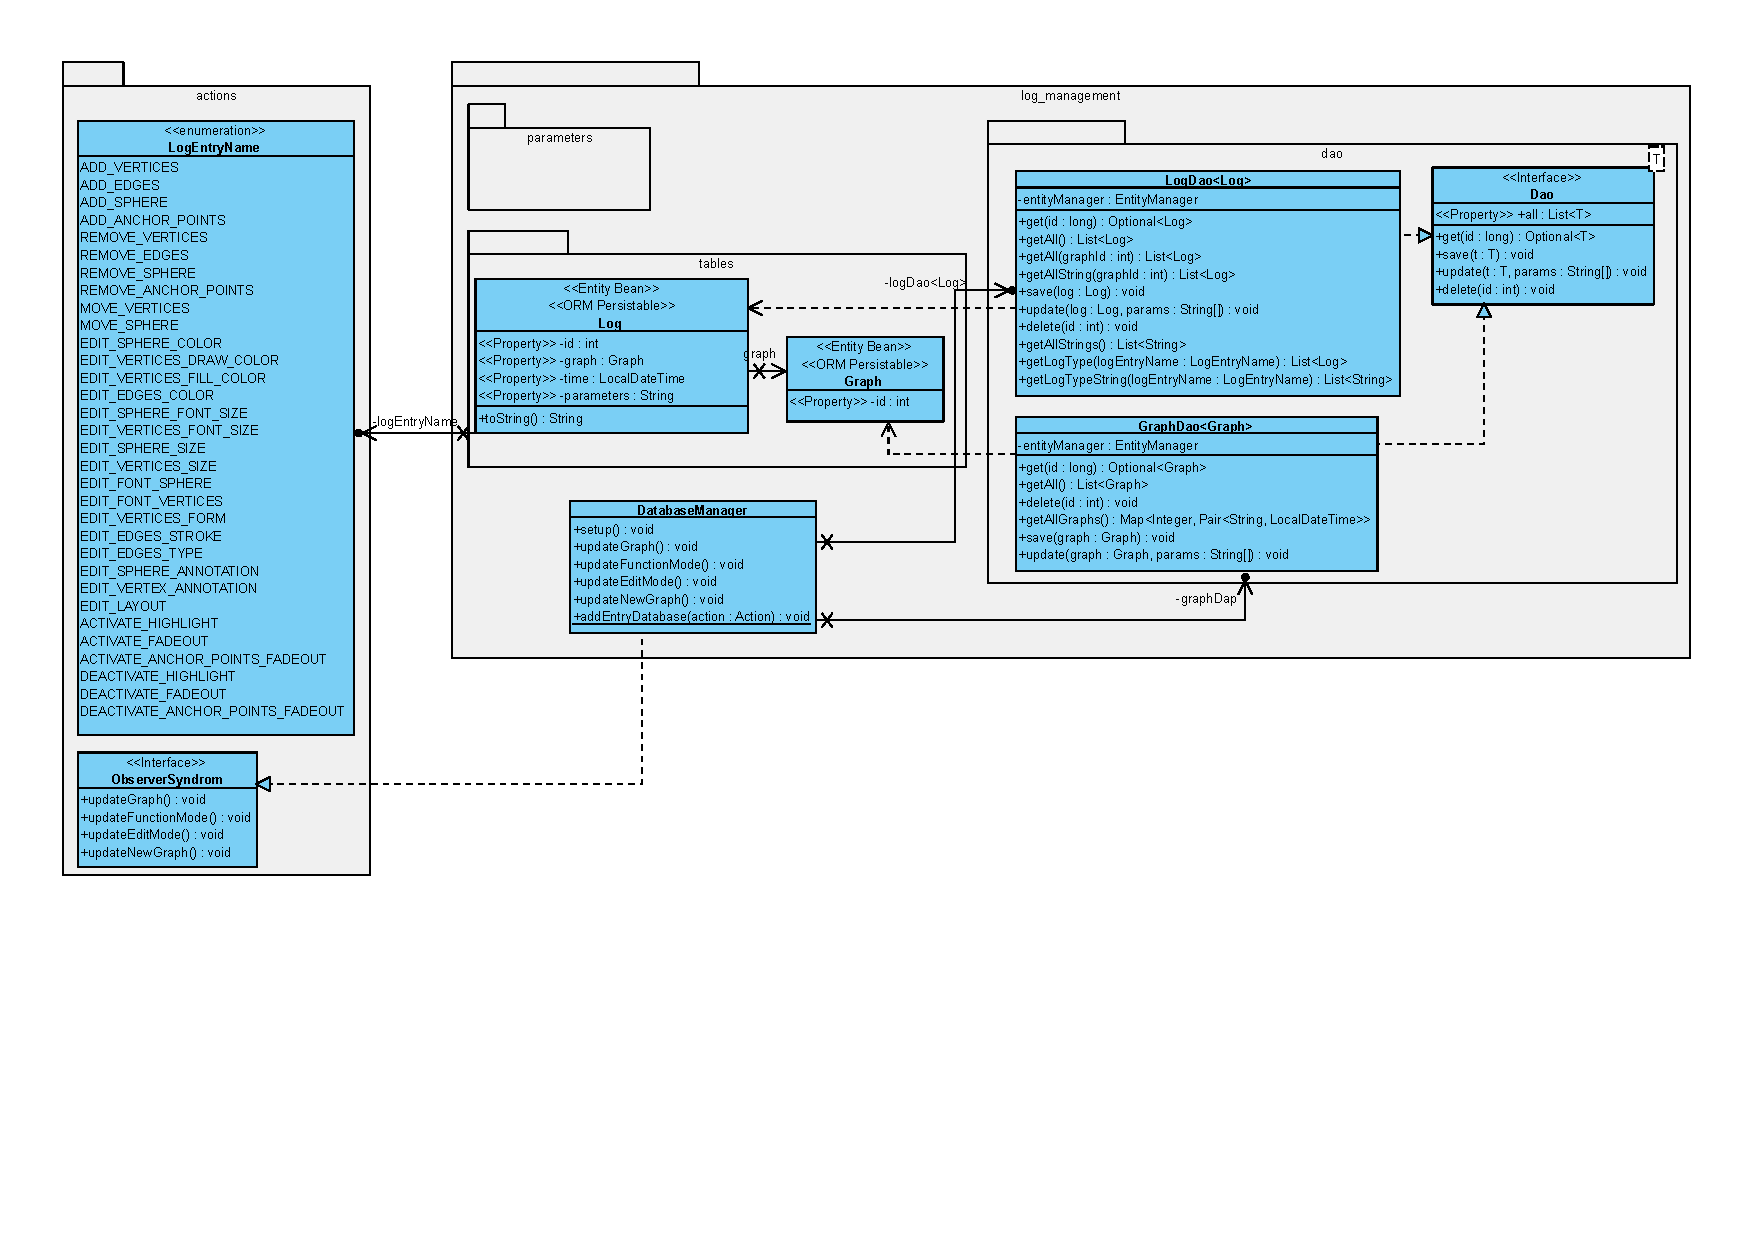
\includepdf[pages=-, landscape, scale=0.84,pagecommand={\pagestyle{fancy}}]{log_management.pdf}



Die \texttt{Param}-Klassen finden sich im Package \texttt{log\_management/parameters}. 
Die Klassen haben individuelle Verbindungen zu Teilen des \texttt{graph/graph}-Packages. So ist beispielsweise die \texttt{EditFontSphereParam} mit \texttt{Sphere}, die \texttt{AddRemoveAnchorPointsParam} mit \texttt{Edge}, die \texttt{EditEdgesTypePram} mit \texttt{EdgeArrowType} und die \texttt{EditVerticesSizeParam} mit \texttt{Vertex} verbunden. \\
Die Klassen innerhalb des Pakets \texttt{graph.graph} sind auf geeignete Weise miteinander verknüpft. \\ 

Die \texttt{Param} Klassen werden benötigt, um die wichtigen Informationen von einer zugehörigen Aktion zu erfassen und in der Datenbank abzuspeichern, damit diese bei Bedarf an den Benutzer übermittelt werden können. Wie genau diese persistiert werden, ist auf der vorherigen Seite beschrieben.\\

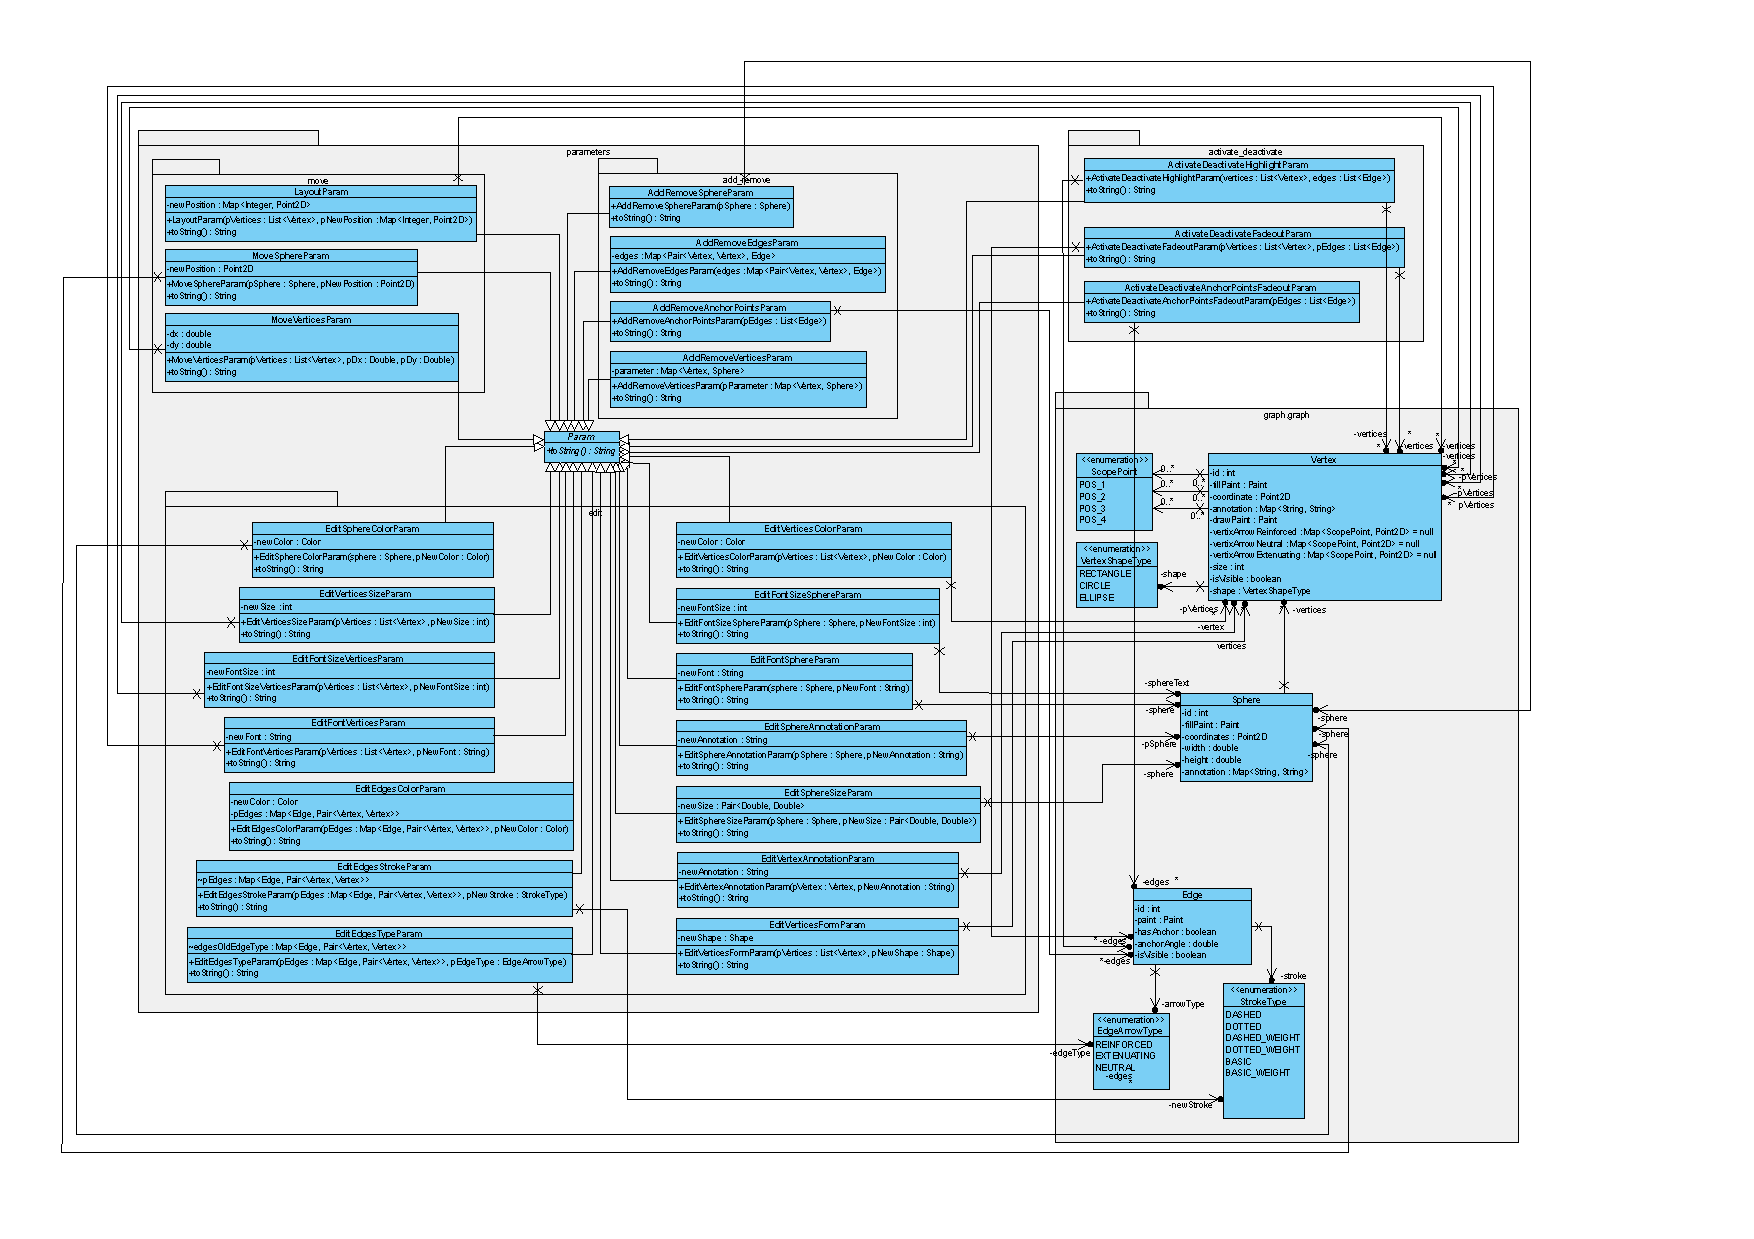
\includepdf[pages=-, landscape, scale=0.84,pagecommand={\pagestyle{fancy}}]{parameters.pdf}



\subsection{Noch zuzuordnen}


Das Zusammenspiel von Im- und Export beziehungsweise von der Erstellung von GXL-, PDF- oder OOF-bezogenen-Aspekten und dem Entwurfsmuster Command besteht darin, dass es Klassen im \texttt{actions.export\_graph-package} gibt, die aus der \texttt{Controller-Klasse} im Package \texttt{gui} (gemäß MVC) aufgerufen werden. Die Methoden in den Klassen des \texttt{export\_graph-packages} wiederum werden später die Methoden der Klassen im package \texttt{io} aufrufen. \\
--> löschen, da nicht gut zu einer Subsection zugehörig und auch etwas redundant, oder?


Um das auf Swing basierende JUNG in die GUI einbinden zu können werden wir die von JavaFX bereitgestellten Swing-Nodes nutzen. Über diese kann die Swing-Komponente in die mit JavaFX erstellte GUI eingebunden werden. Dieses Vorgehen folgt Strategie \hyperlink{lll}{S36 - SwingNode}. Die GUI wird dabei mit dem Scene-Builder erstellt und die dabei erzeugten FXML-Dateien werden in unser System integriert werden (\hyperlink{mmm}{S38 - Scene-Builder}). \\ \\
--> zu graph.graph zuordnen?

Im Zuge der Implementierung unserer Software werden wir die Übersichtlichkeit durch Kombination der Strategien \hyperlink{sss}{S53 - Layouts in Layouts}, \hyperlink{xee}{S54 - JUNG Layouts} und \hyperlink{xff}{S55 - Eigenes Layout} die Übersichtlichkeit im Graphen erhöhen.
--> zu graph.visualisation zuordnen?



\newpage

\subsection{\texttt{graph.graph}}

Das Package \texttt{graph.graph} beinhaltet die Datenklassen des Graphen und Klassen, die sich auf die Funktionalität des Graphen beziehen. \\

Die Klasse \texttt{Syndrom} führt alle Komponenten des Frameworks \hyperlink{eee}{S19 - \texttt{JUNG}} zusammen und ist ein \textit{Singleton}, da dieses Objekt global im ganzen Projekt verfügbar sein muss. \\
Unsere Datenklassen zu dem Graphen erweitern das Datenmodell von \texttt{JUNG}. Klassen, die erweiterte Funktionalität des Graphen implementieren, erweitern meistens Klassen aus \texttt{JUNG} oder orientieren sich an dessen Klassen. \\

\textit{Syndrom} enthält ein \texttt{SyndromGraph} Objekt, ein \texttt{StaticLayout} Objekt und eine \texttt{VisualisationViewer} Objekt, welche die grundlegenden Informationen über den Graphen beinhalten, beispielsweise Listen von \texttt{Vertex}/ \texttt{Edge} und \texttt{Sphere}. Die \texttt{Transformer} Attribute von \texttt{Syndrom} werden aus dem Package \texttt{graph.visualization} importiert und sind vor allem für die Visualisierung von Bedeutung. Die \texttt{Predicate} Attribute von \texttt{Syndrom} werden aus dem Package \texttt{graph.alogorithm} importiert und werden später für die Filterung und Umsetzung von Algorithmen auf den Graphen benötigt. \\

Die Klasse  \texttt{VisualisationViewer} und \texttt{StaticLayout} haben wir komplett von Jung übernommen, wir weisen den generischen Typen der Klassen unsere \texttt{Vertex}/ \texttt{Edge} Objekte zu. Somit sind unsere eigenen Datenklassen nicht  komplett von dem JUNG-Framework unabhängig.\\

Das \texttt{SatelliteVisualisationViewer} Objekt, das \texttt{ViewGrid} und das \texttt{GraphZoomScrollPane} Objekt sind \texttt{JUNG} zugehörige Klassen, die wir benötigen, um \hyperlink{dd}{Zoom} und \hyperlink{ff}{Zoom.Kontext} umzusetzen. Die Klassen \texttt{ViewGrid} werden wir selber implementieren, dies Implementierung ist aber an \texttt{JUNG} Klassen angelehnt.\\

Das Attribut \texttt{pluggable} der Klasse \texttt{PluggableGraphMouse} wird ebenfalls von \texttt{JUNG} zur Verfügung gestellt. Diese Klasse besitzt Funktionalität, um \texttt{GraphMousePlugins} (im Package \texttt{visualisation}) hinzuzufügen und zu entfernen. Diese besitzen Methoden, um MouseEvents auf den \texttt{VisualisationViewer} zu erkennen und Funktionalität entsprechend umzusetzen. \\

Die Klasse \texttt{Syndrom} enthält außerdem ein Attribut \texttt{values}, welches eine Instanz der Klasse \texttt{Values} ist. Die \texttt{GUI} schreibt gesetzte Wert der \texttt{GUI} in die Klasse, z.B. den derzeit gewählten \texttt{EdgeType}. Syndrom benötigt diese Werte, damit Objekte entsprechend dieser Werte erstellt werden können. \\


\newpage

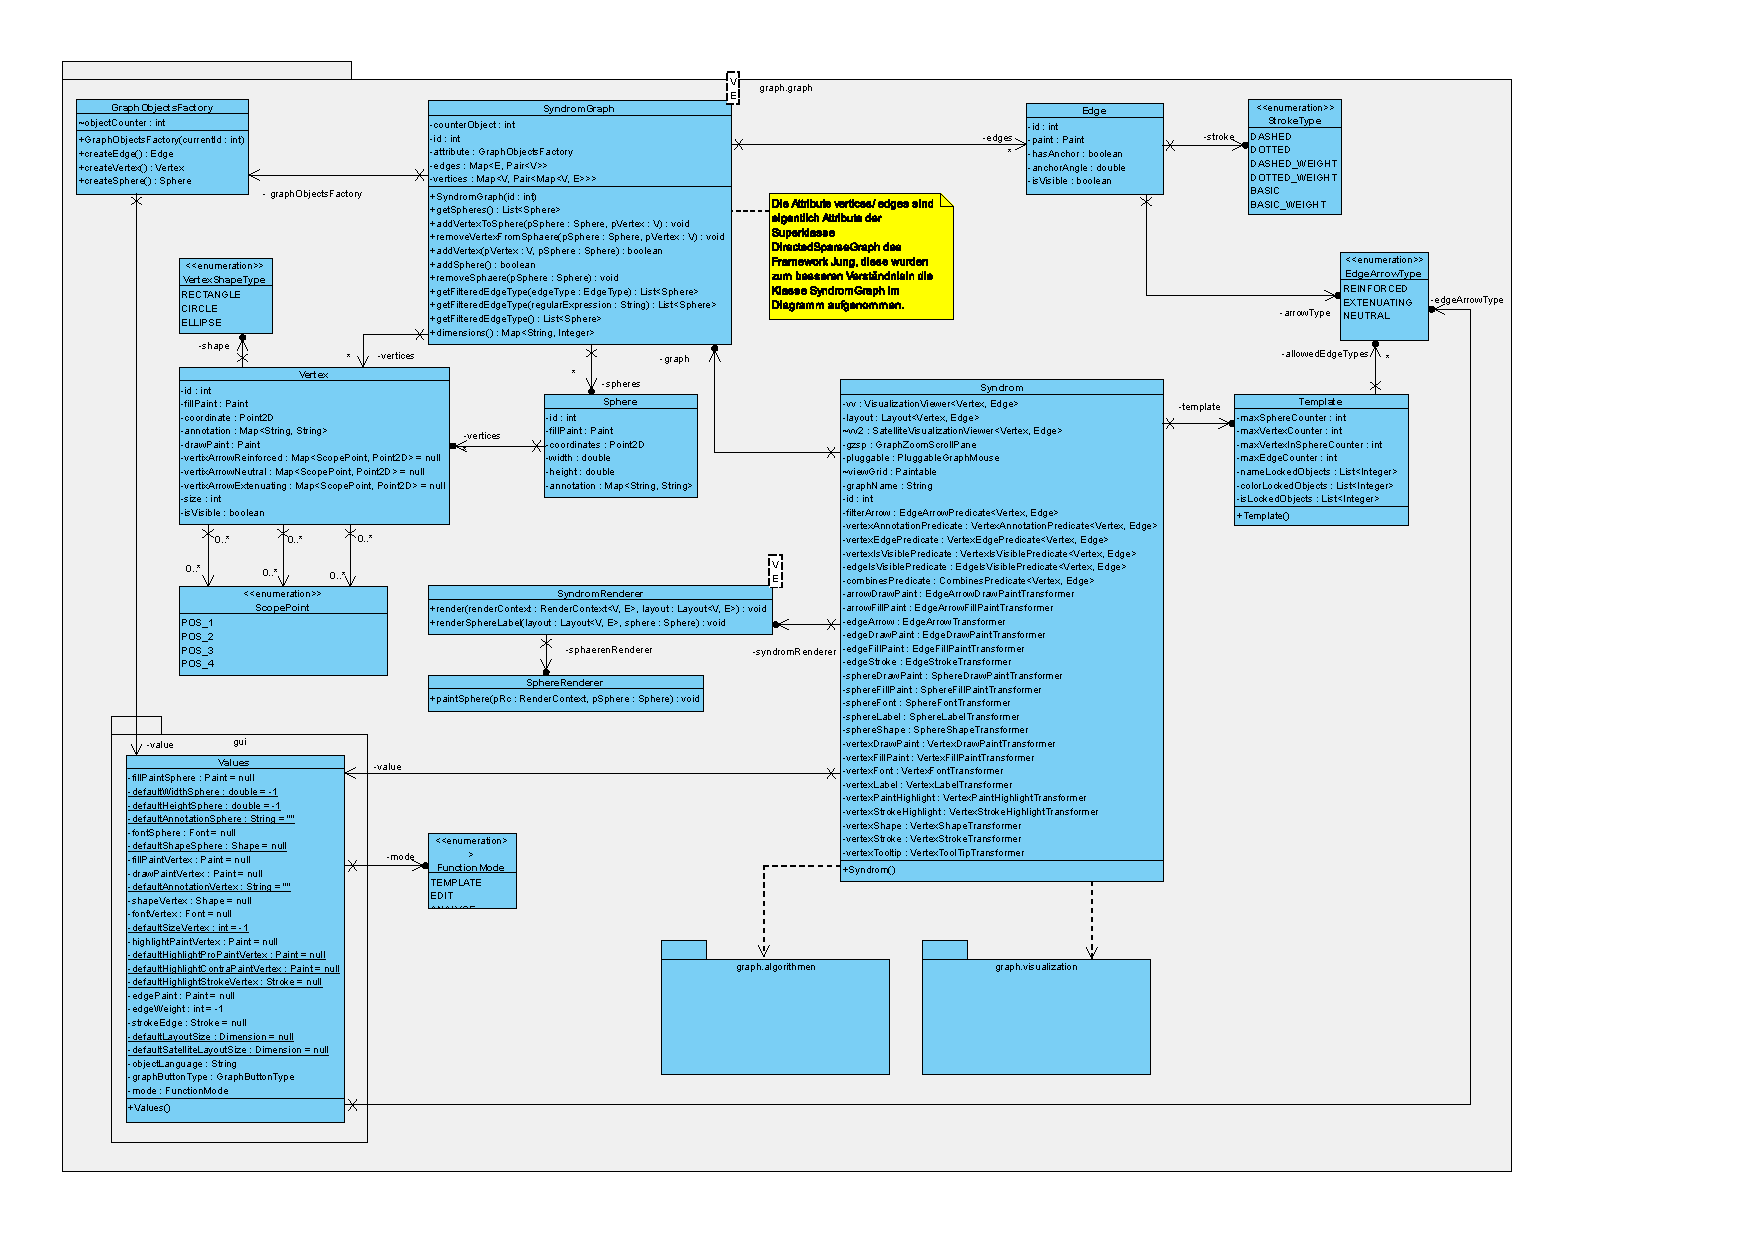
\includepdf[pages=-, landscape, scale=0.84,pagecommand={\pagestyle{fancy}}]{graph_graph.pdf}


\subsection{\texttt{graph.visualization}}

Das Package \texttt{visualization} beinhaltet alle Klassen, die auf die Visualisierung des Graphen Einfluss haben. \\

Ein großes Teilpaket von \texttt{visualsation} sind die Transformer.  Alle diese Klassen implementieren ein Interface \texttt{Transformer}. Diese wandeln ein Eingabe Objekt in ein Ausgabe Objekt um. Das Eingabe Objekt bleibt dabei unverändert. Wir bzw. das Framework \texttt{JUNG} verwendet Transformer größtenteils dazu, um Daten aus Objekten zu extrahieren, beispielsweise die Farbe eines \texttt{Vertex}. \\

Ein weiteres Teilpaket ist \texttt{control}. Die Klassen aus dem Package erben alle von der Klasse \\ \texttt{GraphMousePlugin} aus \texttt{JUNG}. Diese \textit{Plugins} implementieren die Funktionalität, die bestimmt, welche Anweisungen bei z.B. einem Klick auf einem \texttt{VisualisationViewer} ausgeführt werden sollen. \\

\texttt{renderers} beinhaltet eine zentrale Klasse \texttt{SyndromRenderer}, die den \texttt{BasicRenderer} von \texttt{JUNG} erweitert. Diese Klasse wird aufgerufen, wenn der Graph gerendert und auf den \texttt{VisualisationViewer} gezeichnet werden soll. Zusätzlich überschreiben wir die Implementierung von \texttt{BasicEdgeRenderer} und erstellen eine weitere Klasse \texttt{SphereRenderer}, um z.B. das \hyperlink{cc}{Zusammenfassen von Pfeilspitzen} zu ermöglichen. \\

Die Klasse \texttt{SyndromPickSupport} überschreibt ebenfalls eine Klasse aus \texttt{JUNG}: \texttt{ShapePicksupport}. Diese erweitern wir mit der Funktionalität ebenfalls \texttt{Sphere} Objekt picken zu können. \\ 

Das Package \texttt{util} beinhaltet zur Zeit nur eine Klasse, und zwar die Klasse \texttt{SyndromArrowFactory}, welche Shape Objekt generiert, welche unsere Pfeilspitzen der Kanten bilden. \\

\texttt{graph.visualization} importiert Klassen aus dem Package \texttt{graph.graph}, da die Klassen die Objekte, welche sie visualisieren sollen, benötigen. \\



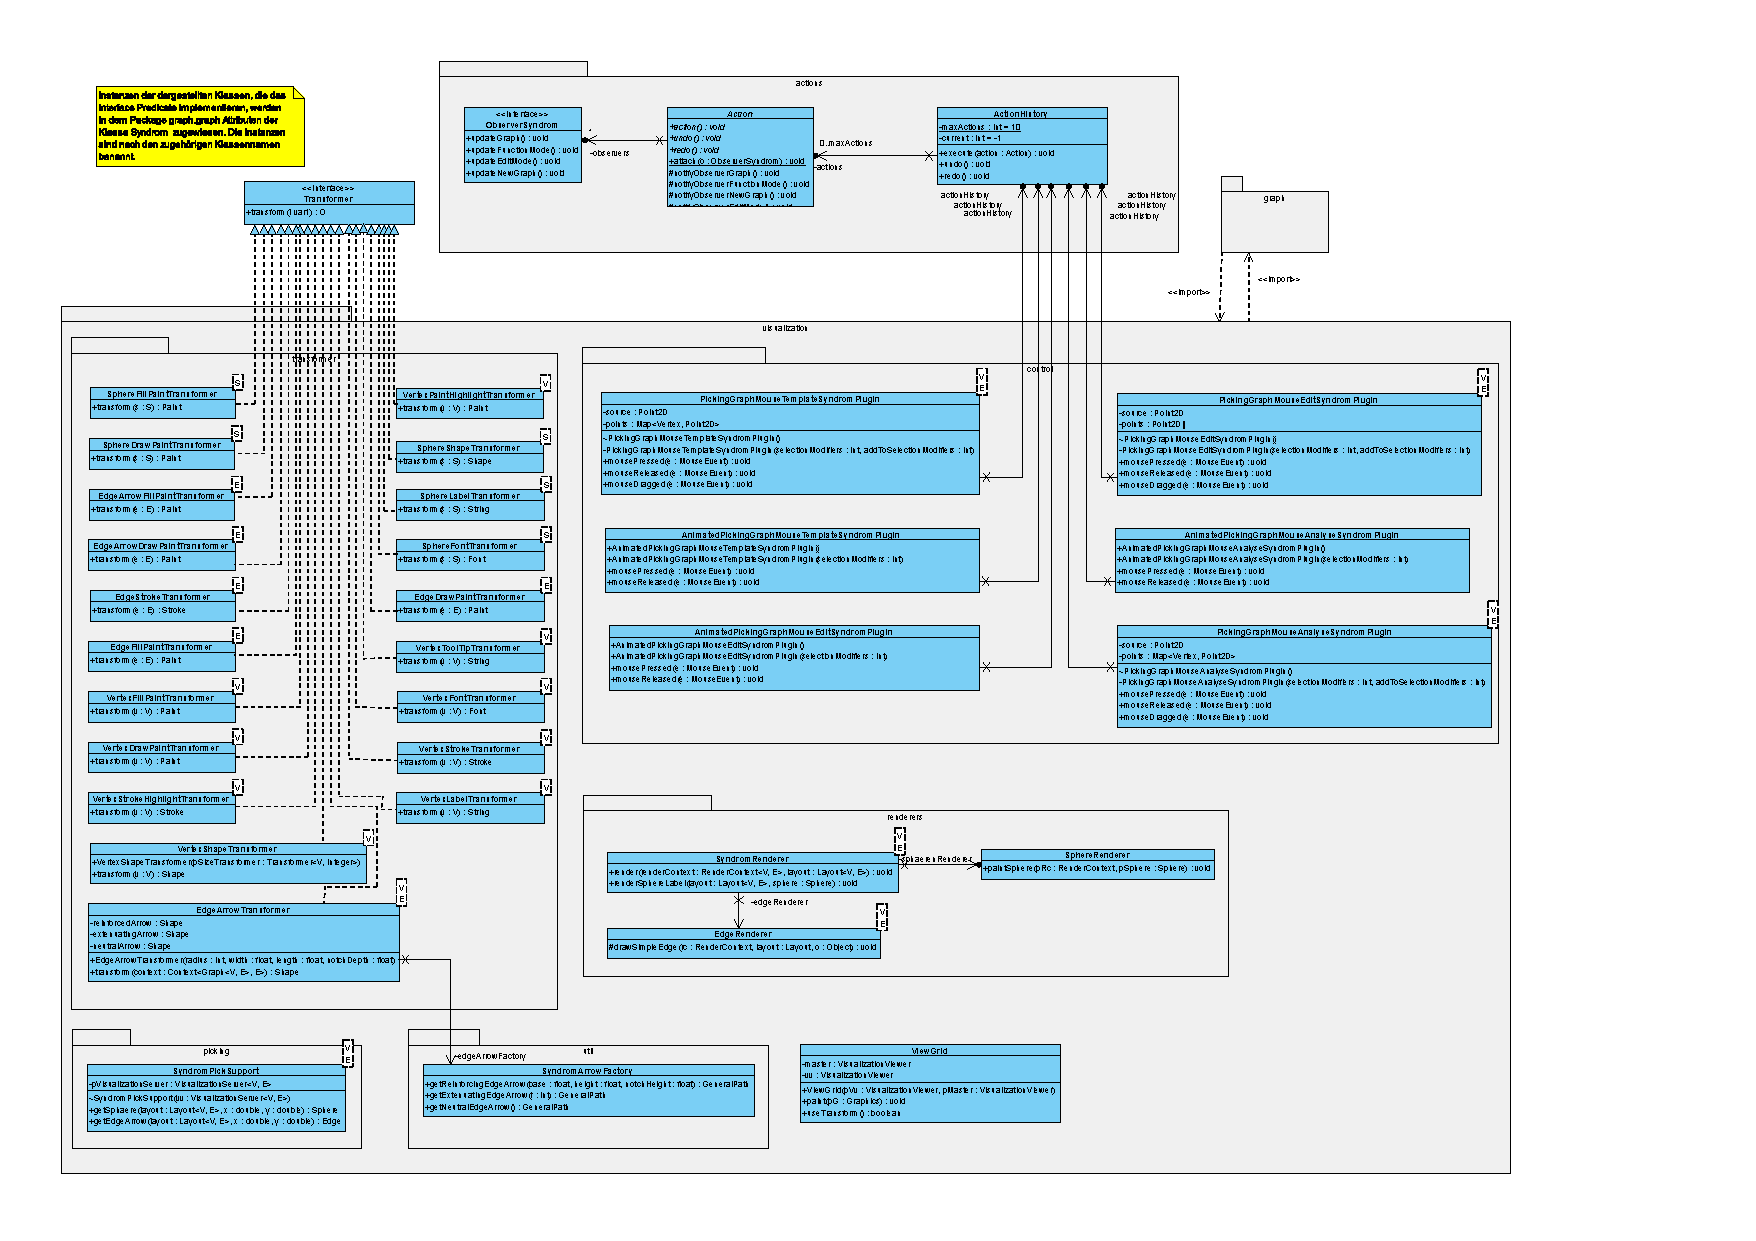
\includepdf[pages=-, landscape, scale=0.84,pagecommand={\pagestyle{fancy}}]{transformer.pdf}

\subsection{\texttt{graph.algorithmen}}
Den größten Teil des Packages \texttt{algorithmen} nimmt das Teilpackage \texttt{predicates} ein. Alle Klassen in \texttt{predicates} implementieren das Interface \texttt{Predicate}. Dieses bietet eine Funktionsschnittstelle, die einen Vergleichstest für ein Objekt ausführt. Es wird entweder \texttt{true} oder \texttt{false} zurückgeben, je nachdem, ob das Objekt den Test besteht oder nicht. \texttt{JUNG} verwendet diese Schnittstelle zur \hyperlink{ss}{Filterung} des Graphen. Nach Strategie \hyperlink{jung}{S66-Jung} implementieren wir alle Algorithmen die zur Analyse/ Auswertung des Graphen benötigt werden soweit wie möglich mit \texttt{Jung} zur Verfügung gestellte Funktionen und Algorithmen. \\

Zusätzlich gibt es nur drei \textit{Enum} Klassen. Diese verwenden wir um zu differenzieren welche Filterung des Graphen durchgeführt werden soll. Bei einer Filterung auf Grundlage \texttt{AnalyseTypeSeveral} - Enumerationskonstanten, können mehrere kombiniert werden, sodass eine kombinierte Filterung ausgeführt wird. Bei \texttt{AnalyseTypeSingle} - Enumerationskonstanten immer nur genau eine. \texttt{SelectionType} beschreibt die verschiedenen Selectionsarten. \\

\texttt{algorithmen} importiert Klassen des Packages \texttt{graph}, da bei einer Filterung die Klasse natürlich Zugriff auf die Objekte benötigt, die gefiltert werden sollen.\\


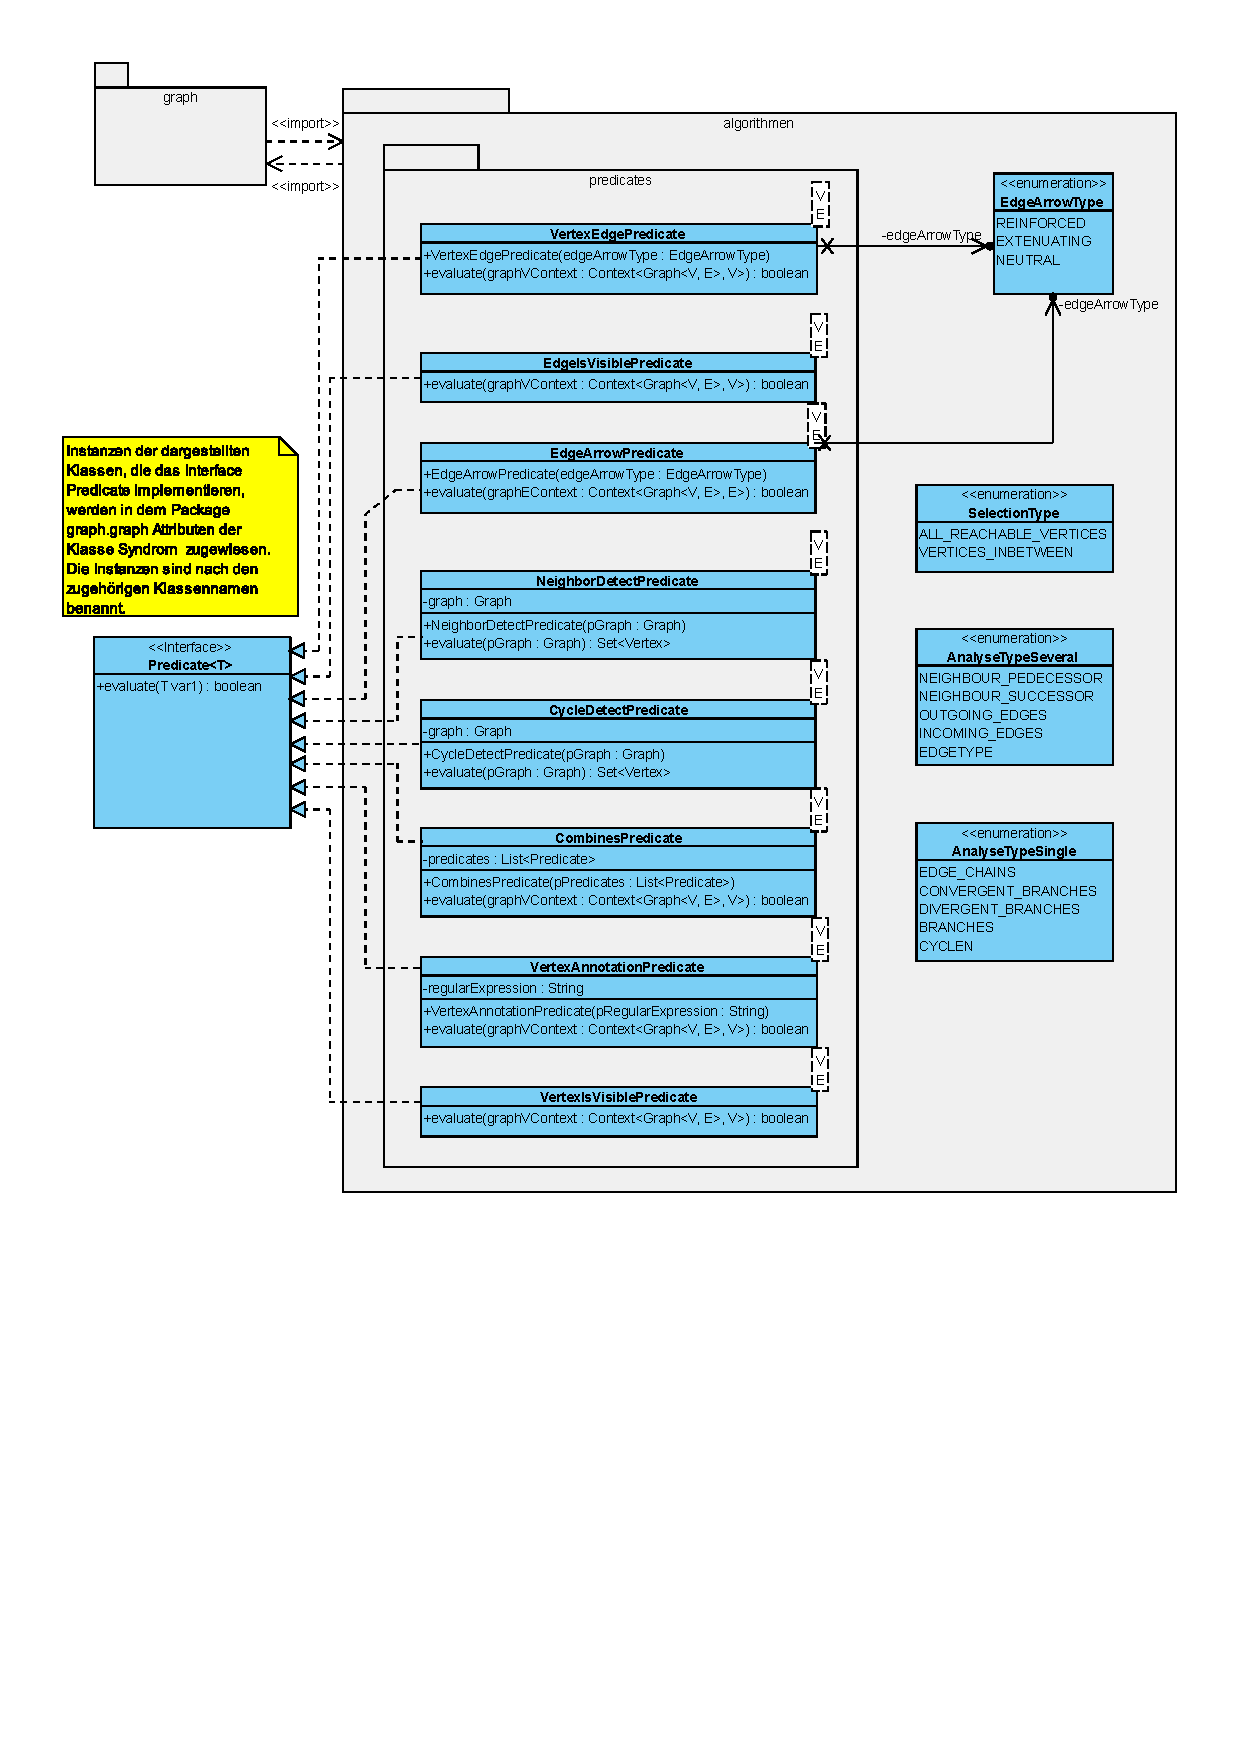
\includepdf[pages=-, scale=0.84,pagecommand={\pagestyle{fancy}}]{predicates.pdf}



\subsection{\texttt{jgrapht}}
In unserem Programm soll neben dem Editieren des Graphen auch das Auswerten des Graphen von großer Bedeutung sein. Für das Auswerten des Graphen müssen bestimmte Algorithmen zur Verfügung stehen.\\ Manche Algorithmen (z.B. Zyklensuche im Graph) sind nach Strategie \hyperlink{xxx}{S69 - JGraphT} in dem Framework JGraphT implementiert, da sie nicht durch \textit{JUNG} zur Verfügung gestellt werden. Die Nutzung der Algorithmen lässt sich in dem Package \texttt{JGraphT} wiederfinden.\\
Da aber unser Datenmodell des Graphen nicht mit dem kompatibel ist welche JGraphT benutzt, muss der Graph zuerst in das andere Modell übersetzt werden. Die Methode \texttt{convertGraphToJGraphT} realisiert diese Funktion. Die Ergebnismenge der Algorithmen werden als \texttt{Set<Vertex>} oder \texttt{List<Vertex>} zurückgegeben, wobei die Klasse \texttt{Vertex} der Klasse \texttt{Vertex} unseres ursprünglichen Modells entspricht. 
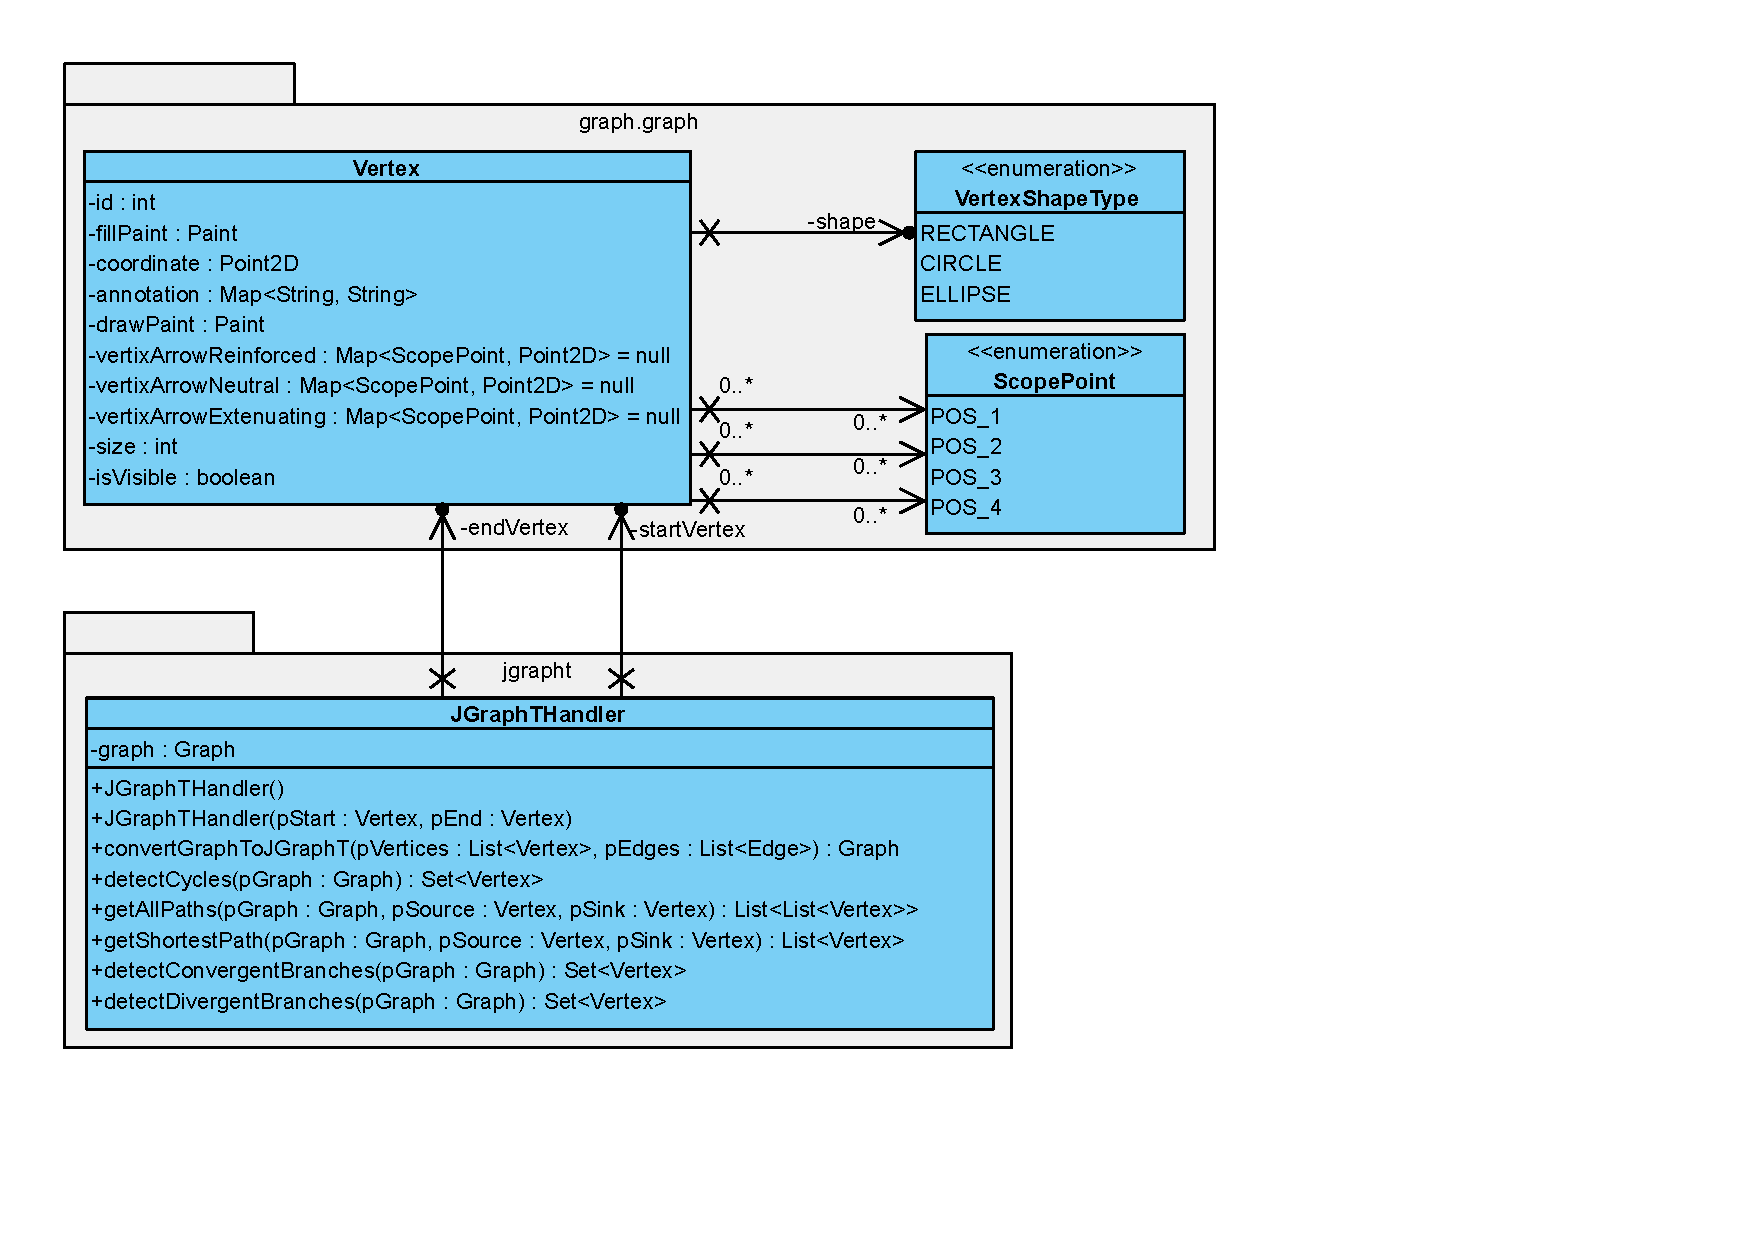
\includepdf[pages=-, landscape, scale=0.84,pagecommand={\pagestyle{fancy}}]{jgrapht.pdf}





Zusammenhang zwischen Modulsicht und konzeptioneller Sicht: Wie im Abschnitt zur GUI-Komponente  in der konzeptionellen Sicht und eben unter Bezugnahme auf verwendete Strategien erwähnt wird die GUI mit JavaFX umgesetzt. Der Bezug zur JUNG-Komponente besteht in der Einbettung derselben über Swing-Nodes. Die Aufteilung des übergeordneten Packages \texttt{graph} in die untergeordneten Packages \texttt{graph}, \texttt{visualization} und \texttt{algorithmen} ist an die konzeptionelle Sicht angelehnt. Dort wurde die beschrieben, dass wir von der JUNG-Komponente die Bereiche \texttt{graph} und \texttt{visualization}  nutzen. Darüber hinaus existiert die Komponente JGraphT, die wir für die Auswertung des Graphen nutzen wollen und die im Package \texttt{algorithmen} umgesetzt werden wird. Die Command-Komponente entspricht dem \texttt{actions-package}. Bei der Umsetzung der Undo-/Redo-Funktionalität, deren Existenz in der konzeptionellen Sicht bereits angedeutet wurde, wird die Klasse \texttt{Action History} im package \texttt{actions} eine wichtige Funktion übernehmen. Die Kommunikation von Commands und der GXL-Komponente (die Logik letzterer wird in der GXLio-Klasse umgesetzt werden) wurde in der konzeptionellen Sicht beschrieben. Das Model-View-Controller Design-Pattern wurde bereits in der konzeptionellen Sicht erwähnt. Auf die Modulsicht angewandt lässt es sich in folgender Kommunikationskette wiederfinden. Der Nutzer interagiert mit Elementen der View (umgesetzt im Package \texttt{gui}). Dadurch werden Controller (in unserem Fall Commands – umgesetzt in Form der Klassen des Packages \texttt{actions} aufgerufen. Diese rufen die Funktionalität folgender Packages auf, die ihrerseits die eigentliche Logik umsetzen und zum Teil auch unsere Models repräsentieren: \texttt{graph}, \texttt{jgrapht} und \texttt{io}. Die Commands / Actions kommunizieren außerdem mit der Persistence, die wir im Package \texttt{log\char`_management} umgesetzt haben. Die Komponenten PDF und FreeHeb VectorGraphics finden sich im \texttt{io}-Package in der Klasse \texttt{PDFio} wieder. Die JGrapT-Komponente findet sich im Package \texttt{jgrapht}  wieder.



\newpage
\section{Ausführungssicht}
\label{sec:ausfuehrung}
\emph{Autoren: Jonah Jaeger}\\ \\
 
{\it
Die Ausführungssicht beschreibt das Laufzeitverhalten. Hier
werden die Laufzeitelemente aufgeführt und beschrieben, welche Module
sie zur Ausführung bringen. Ein Modul kann von mehreren
Laufzeitelementen zur Laufzeit verwendet werden. Die Ausführungssicht
beschreibt darüber hinaus, welche Laufzeitelemente spezifisch
miteinander kommunizieren. Zudem wird bei verteilten Systemen
(z.\,B. Client-Server-Systeme) dargestellt, welche Module von welchen
Prozessen auf welchen Rechnern ausgeführt werden.}\\ \\

\begin{figure}[ht]
	\centering
	\includegraphics[width=1\textwidth]{ausfuehrungssicht.png}
	\caption{Ausführungssicht}
\end{figure}

\newpage{}
\section[Zusammenhänge zwischen Anwendungsfällen und Architektur]{Zusammenhänge zwischen Anwendungsfällen und Architektur\sectionmark{Zusammenhänge AF u. Architektur}}
\sectionmark{Zusammenhänge AF u. Architektur}
\label{sec:anwendungsfaelle}
\emph{Autoren: Jacky Philipp Mach, Jonah Jaeger, Clement Phung}\\ \\

\subsection{Anwendungsfall: Ein Lehrer erstellt einen Syndromansatz}

\begin{tabular} {|p{16cm}|}
	\hline
	\rowcolor{anw}\parbox{16cm}{\textbf{A1: Ersteller erstellt Syndromansatz}} \\\hline
	\hline
	\textbf{Akteure}: Ersteller
	\\\hline
	\textbf{Vorbedingungen}: Das Programm ist geöffnet. Der Ersteller hat schon vorher mit dem Programm gearbeitet. \\
	\textit{Ziel}: Einen neuen Syndromansatz erstellen.
	\\\hline
		\textbf{Regulärer Ablauf}: \begin{itemize}
		\itemsep-0.5em
		\item der Ersteller drückt auf den Menüpunkt \textit{Datei}  $\rightarrow$ \textit{Neuen Graph erstellen}
		\item das System öffnet zwei Pop-Up-Fenster (Abfrage für Speichern des alten Graphen und Eingabefeld des Namen des neuen Graphen) 
		\item \textbf{der Ersteller gibt den Namen des Graphen an und klickt ok}
	\end{itemize}
	\\\hline
	\textbf{Varianten}: Der Ersteller könnte Elemente zu dem Graphen hinzufügen und diese miteinander verknüpfen.
	\\\hline
	\textbf{Nachbedingung}: Der Ersteller hat einen Graph erstellt. Dieser Graph kann der Ersteller nun beliebig bearbeiten und speichern/exportieren.
	\\\hline
	\textbf{Fehler-/Ausnahmefälle}:  Der Ersteller könnte vergessen den alten Graphen zu speichern, sodass beim Erstellen des neuen Graphen der alte Graph überschrieben wird.
	\\\hline
\end{tabular}
\\ \\ \\
Der eben beschriebene Anwendungsfall ist im dem folgenden Sequenzdiagramm dargestellt. \\
Da als Vorbedingung angegeben war, dass der User bereits mit dem Programm gearbeitet hat, sind alle Singleton Klassen bereits initialisiert und im Projekt verfügbar. \\
Im Laufe des Sequenzdiagramms wird eine \texttt{CreateGraphAction} erzeugt, die bei Ausführung, das im Programm aktuelle Syndrom Objekt mit einem neuen Graphen/ Layout belegt. Folgend werden die \texttt{GUI} und der \texttt{DatabaseManager} \textit{benachrichtigt}, dass ein neuer Graph erstellt wurde. \\
Im Methodenaufruf des \texttt{DatabaseManagers} wird die Graph- Tabelle unserer Datenbank geleert, da unser Programm intern immer nur eine Graph Repräsentation speichert. \\
Danach wird ein neuer Graph erstellt und das Syndrom Objekt, als Gxl- String in der Graph- Tabelle gespeichert. 

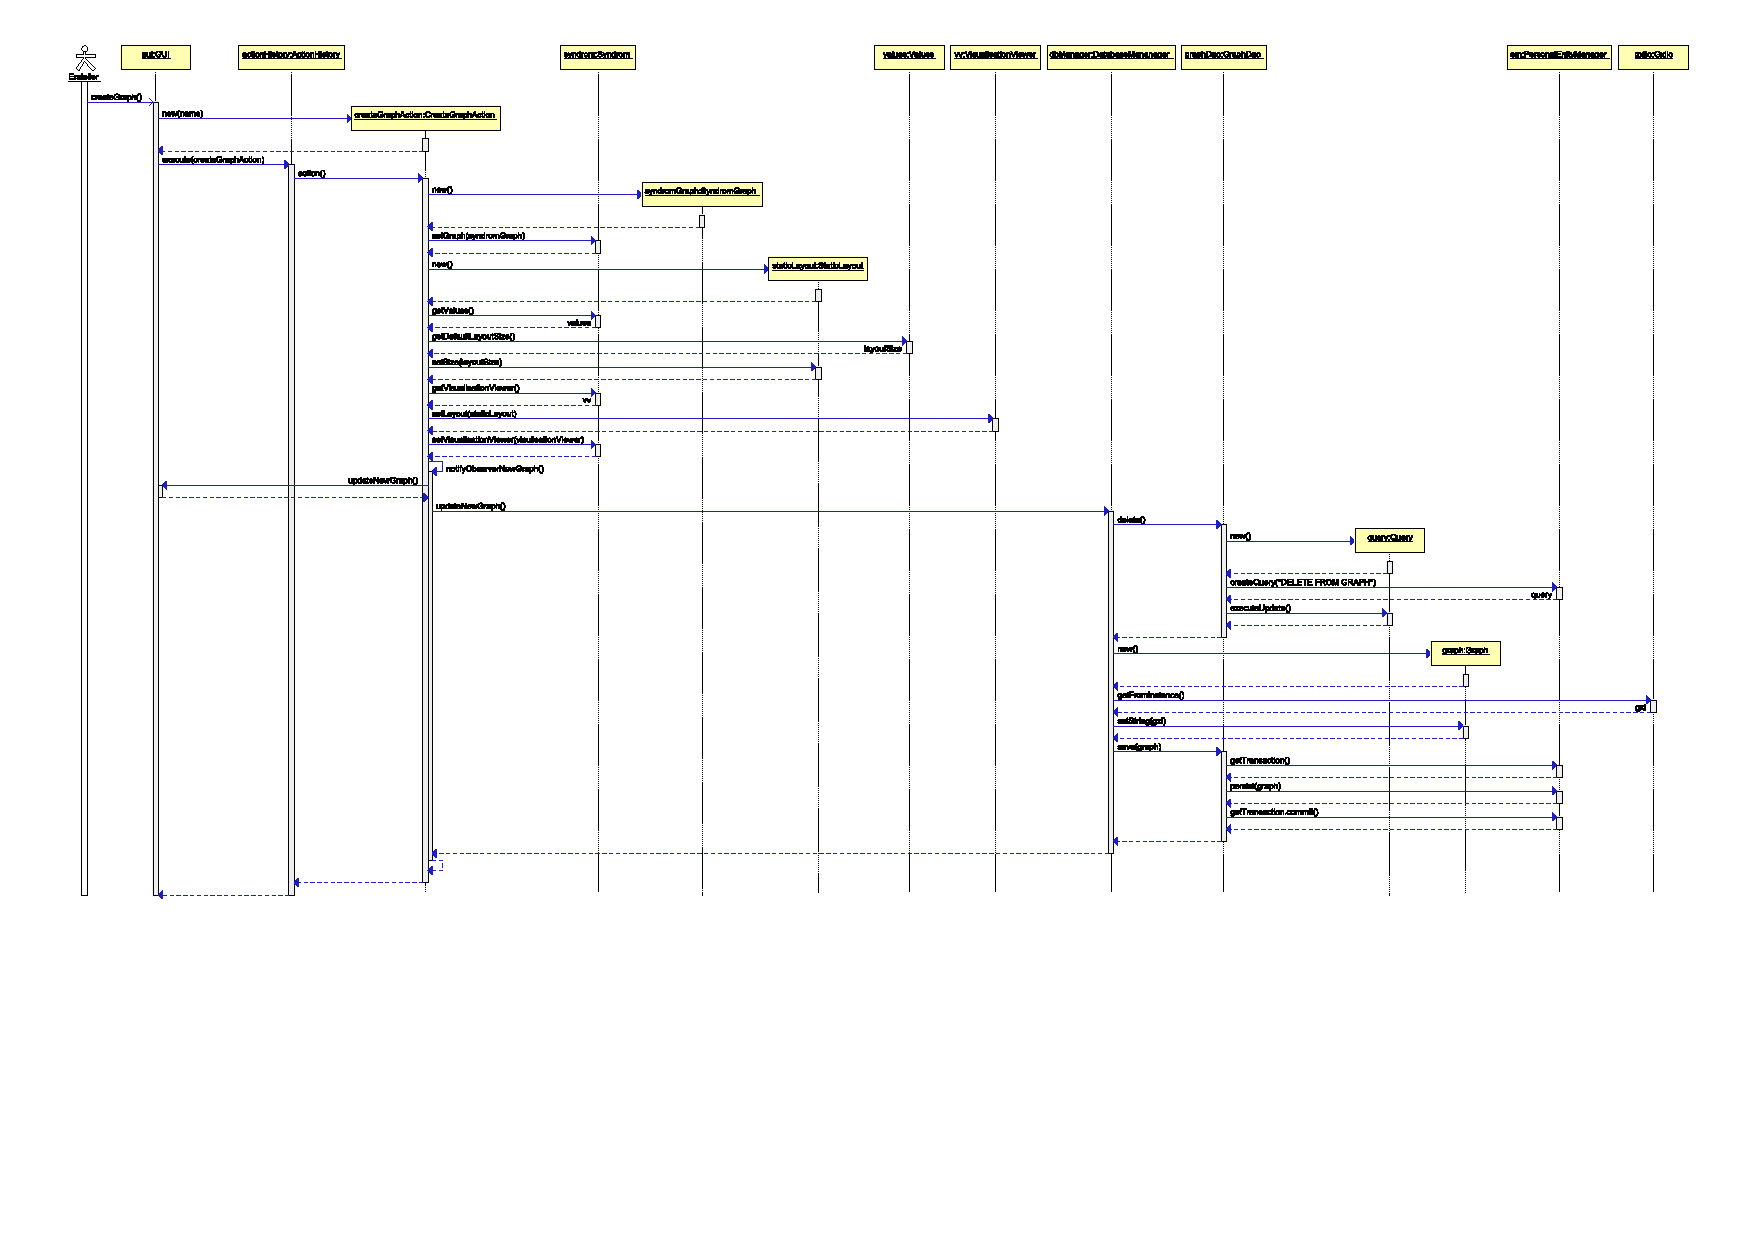
\includepdf[pages=-, landscape, scale=0.84,pagecommand={\pagestyle{fancy}}]{first_.pdf}


\subsection{Anwendungsfall: Ein Lehrer fügt eine Sphäre hinzu}

\begin{tabular} {|p{16cm}|}
	\hline
	\rowcolor{anw}\parbox{16cm}{\textbf{A2: Bearbeiter fügt eine Sphäre hinzu}} \\\hline
	\hline
	\textbf{Akteure}: Bearbeiter
	\\\hline
	\textbf{Vorbedingungen}: Das Programm ist geöffnet, eine GXL-Datei wurde schon erfolgreich importiert. Die Arbeitsfläche ist leer. \\
	\textit{Ziel}: Eine Sphäre hinzufügen.
	\\\hline
		\textbf{Regulärer Ablauf}: \begin{itemize}
		\itemsep-0.5em
		\item der Bearbeiter klickt auf den \textit{Sphäre hinzufügen}- Button
		\item der Bearbeiter klickt in die Arbeitsfläche 
	\end{itemize}
	\\\hline
	\textbf{Varianten}: Der Bearbeiter könnte der Sphäre eine Bezeichnung geben oder mehrere Sphären zu dem Graphen hinzufügen.
	\\\hline
	\textbf{Nachbedingung}: Der Bearbeiter hat eine Sphäre hinzugefügt. Danach kann der Bearbeiter weitere Elemente hinzufügen oder den Graphen exportieren.
	\\\hline
	\textbf{Fehler-/Ausnahmefälle}:  Der Ersteller könnte die Sphäre an eine nicht geeignete Stelle setzen $\rightarrow$ Der Ersteller kann die Sphäre mithilfe des \textit{Sphäre löschen}-Buttons die Sphäre löschen und neu setzen. 
	\\\hline
\end{tabular}
\\ \\ \\

Da zuvor schon Aktion ausgeführt worden sind, sind alle Singleton Objekte bereits initialisiert. \\
Der eben beschriebene Anwendungsfall ist im dem folgenden Sequenzdiagramm dargestellt. \\
Zu Beginn klickt der Ersteller den Button, um eine Sphäre hinzuzufügen. Die \texttt{GUI} schreibt daraufhin den \texttt{GraphButtonTyp} in \texttt{Values}, damit das \texttt{PickingGraphMouseEditSyndromPlugin} weiß, welche Aktion bei Klick in den \texttt{Visualisation Viewer} ausgeführt werden soll. \\
Klickt der Ersteller nun in die SwingNode, also den  \texttt{Visualisation Viewer}, wird die Aktion\\ \texttt{AddSpereLogAction} erstellt und durch die \texttt{ActionHistory} ausgeführt. \\
Bei der Ausführung der Aktion wird das neue \texttt{Sphere} Objekt erstellt und dem Graphen hinzugefügt. \\
Außerdem wird ein \texttt{AddRemoveSphereParam} Objekt erzeugt, welche die eben erstelle \texttt{Sphere} übergeben bekommt. \\
Folgend wird der \texttt{DatabaseManager} und die \texttt{GUI} benachrichtigt, dass sich der Graph verändert hat. \\
Der \texttt{DatabaseManager} updated die Graph Repräsenation in der Datenbank, indem ein neuer GXL- String des Graphen erzeugt und abgespeichert wird.\\
Die \texttt{AddSpereLogAction} wird außerdem als \texttt{Log} Objekt in der Datenbank persistiert, um das Nutzerinteraktionsprotokoll aktuell zu halten. \\
Hierzu werden dem \texttt{LogDao} das \texttt{Log} Objekt und seine Parameter übergeben. Die Parameter werden durch Jackson zu einem Json-String konvertiert und das \texttt{Log} Objekt wird in der Datenbank durch Hibernate abgespeichert.


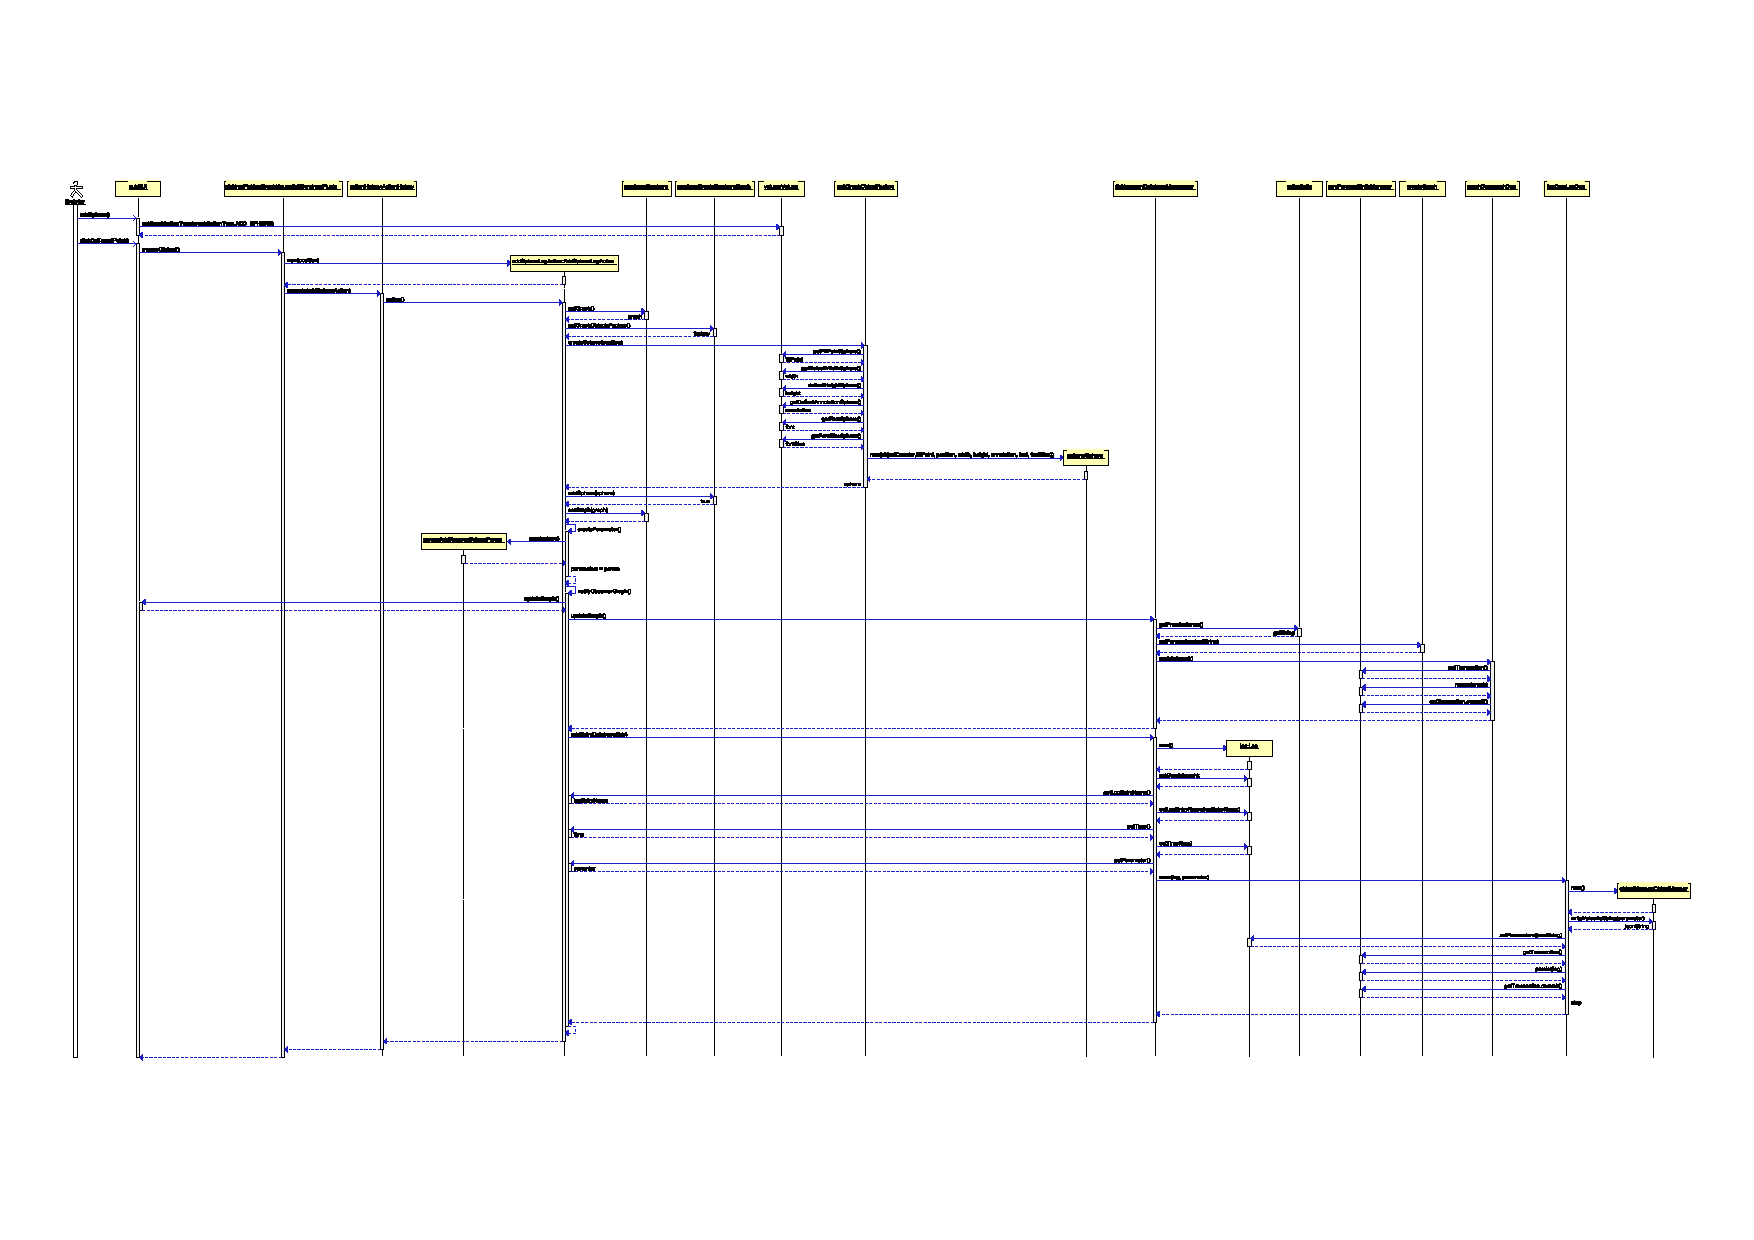
\includepdf[pages=-, landscape, scale=0.84,pagecommand={\pagestyle{fancy}}]{second.pdf}







\newpage

\subsection{Anwendungsfall: Ein/e Schüler/in arbeitet mit der Vorlage seines/r Lehrer/in}

\begin{tabular} {|p{16cm}|}
	\hline
	\rowcolor{anw}\parbox{16cm}{\textbf{A3: Bearbeiter modifiziert Vorlage}} \\\hline
	\hline
	\textbf{Akteure}:  Bearbeiter
	\\\hline
	\textbf{Vorbedingungen}: Das Programm ist geöffnet, die Vorlage in Form einer GXL-Datei ist schon importiert. Diese eine Sphäre.\\ 
	\textit{Ziel}: Vorlage modifizieren und als neuen Datentyp speichern.
	\\\hline
	\textbf{Regulärer Ablauf}:
\begin{itemize}
	\itemsep-0.5em
	\item der Bearbeiter klickt auf den Menüpunkt \textit{Knoten hinzufügen}
	\item der Bearbeiter klickt auf eine Sphäre
	\item der Bearbeiter wählt \textit{Datei} $\rightarrow$ \textit{Exportieren als} $\rightarrow$ \textit{OOF}
	\item der Bearbeiter gibt einen Speicherpfad an und drück den Button \textit{exportieren}
\end{itemize}
	\\\hline
	\textbf{Varianten}: Dem Bearbeiter kann mit vielen Werkzeugen den Graph nach seinen/ihren Wünschen bearbeiten.  
	\\\hline
	\textbf{Nachbedingung}: Die Vorlage wurde modifiziert und als \textit{oof} Datei gespeichert. Der Bearbeiter könnte nun in den Auswertermodus wechseln und dort den Graphen auswerten.
	\\\hline
	\textbf{Fehler-/Ausnahmefälle mit deren Nachbedingung}: Der Bearbeiter vergisst die Datei zu exportieren oder gar zu speichern $\rightarrow$ Beim erneuten Start kann er die Vorlage neu importieren und neu beginnen.
	\\\hline
\end{tabular}\\ \\ \\

Auch hier sind wie im Anwendungsfall oben alle Singleton Objekte schon initialisiert. Zu Beginn des Anwendungsfalles klickt der Bearbeiter auf den Button\texttt{Knoten hinzufügen}. Die Benutzeroberfläche reagiert darauf mit dem Schreiben des \texttt{GraphButtonTyp} in \texttt{Values}, um das \texttt{PickingGraphMouseEditSyndromPlugin} zu signalisieren, was bei einem Klick auf den \texttt{VisualisationViewer} passiert.\\
Die Aktion \texttt{AddVerticesLogAction} wird erstellt, wie bei allen anderen Actions auch, und von der \texttt{ActionHistory} ausgeführt. Durch die \texttt{GraphObjectFactory} wird der Knoten erstellt und in den Graphen hinzugefügt. Während der Action wird das Parameterobjekt \texttt{AddVerticesParam} erstellt und an die Action abgegeben.\\  
Da sich der Graph verändert hat, muss wie im oberen Fall auch, der \texttt{DatabaseManager} und die Benutzeroberfläche benachrichtigt werden. Nach jeder Action, also auch nach dieser, wird der Graph neu als GXL-String in die Datenbank persistiert. Auch muss für die Protokollierung des Benutzers eine neue \texttt{Log} erstellt und in die Datenbank persistiert werden. Dem \texttt{LogDao} werden wieder die Log und die Parameter übergeben. Die Parameter werden zu einem Json-String konvertiert und mit dem Log mithilfe von Hibernate in die Datenbank gespeichert.\\
Nun besteht noch die Action, bei dem ein Benutzer den bestehenden Graphen als OOF exportiert. Bei dem Klick auf den Button \textit{Exportieren als} $\rightarrow$ \textit{OOF}, öffnet die \texttt{GUI} ein Dialogfenster, bei dem der Nutzer einen validen Pfad eingeben und mit dem Button \textit{Exportieren} dies bestätigen muss. \\
Die neue Action \texttt{exportOofAction} wird erstellt und wieder durch die \texttt{ActionHistory} ausgeführt. Ein neues Objekt der Klasse \texttt{OOFIo} wird erstellt. Von dem Objekt wird eine neue \texttt{GXLIo} kreiert und welche den Graphen als GXL-String zurückliefert. Die Logeinträge werden von dem \texttt{LogDao} und die Parameterobjekte von dem bestehendem \texttt{ObjectMapper} in Strings umgewandelt. In der \texttt{OOFIo} werden dann alle Strings mit der Methode \texttt{createOOf()} zu dem neuen Datentyp fusioniert und abgespeichert.  


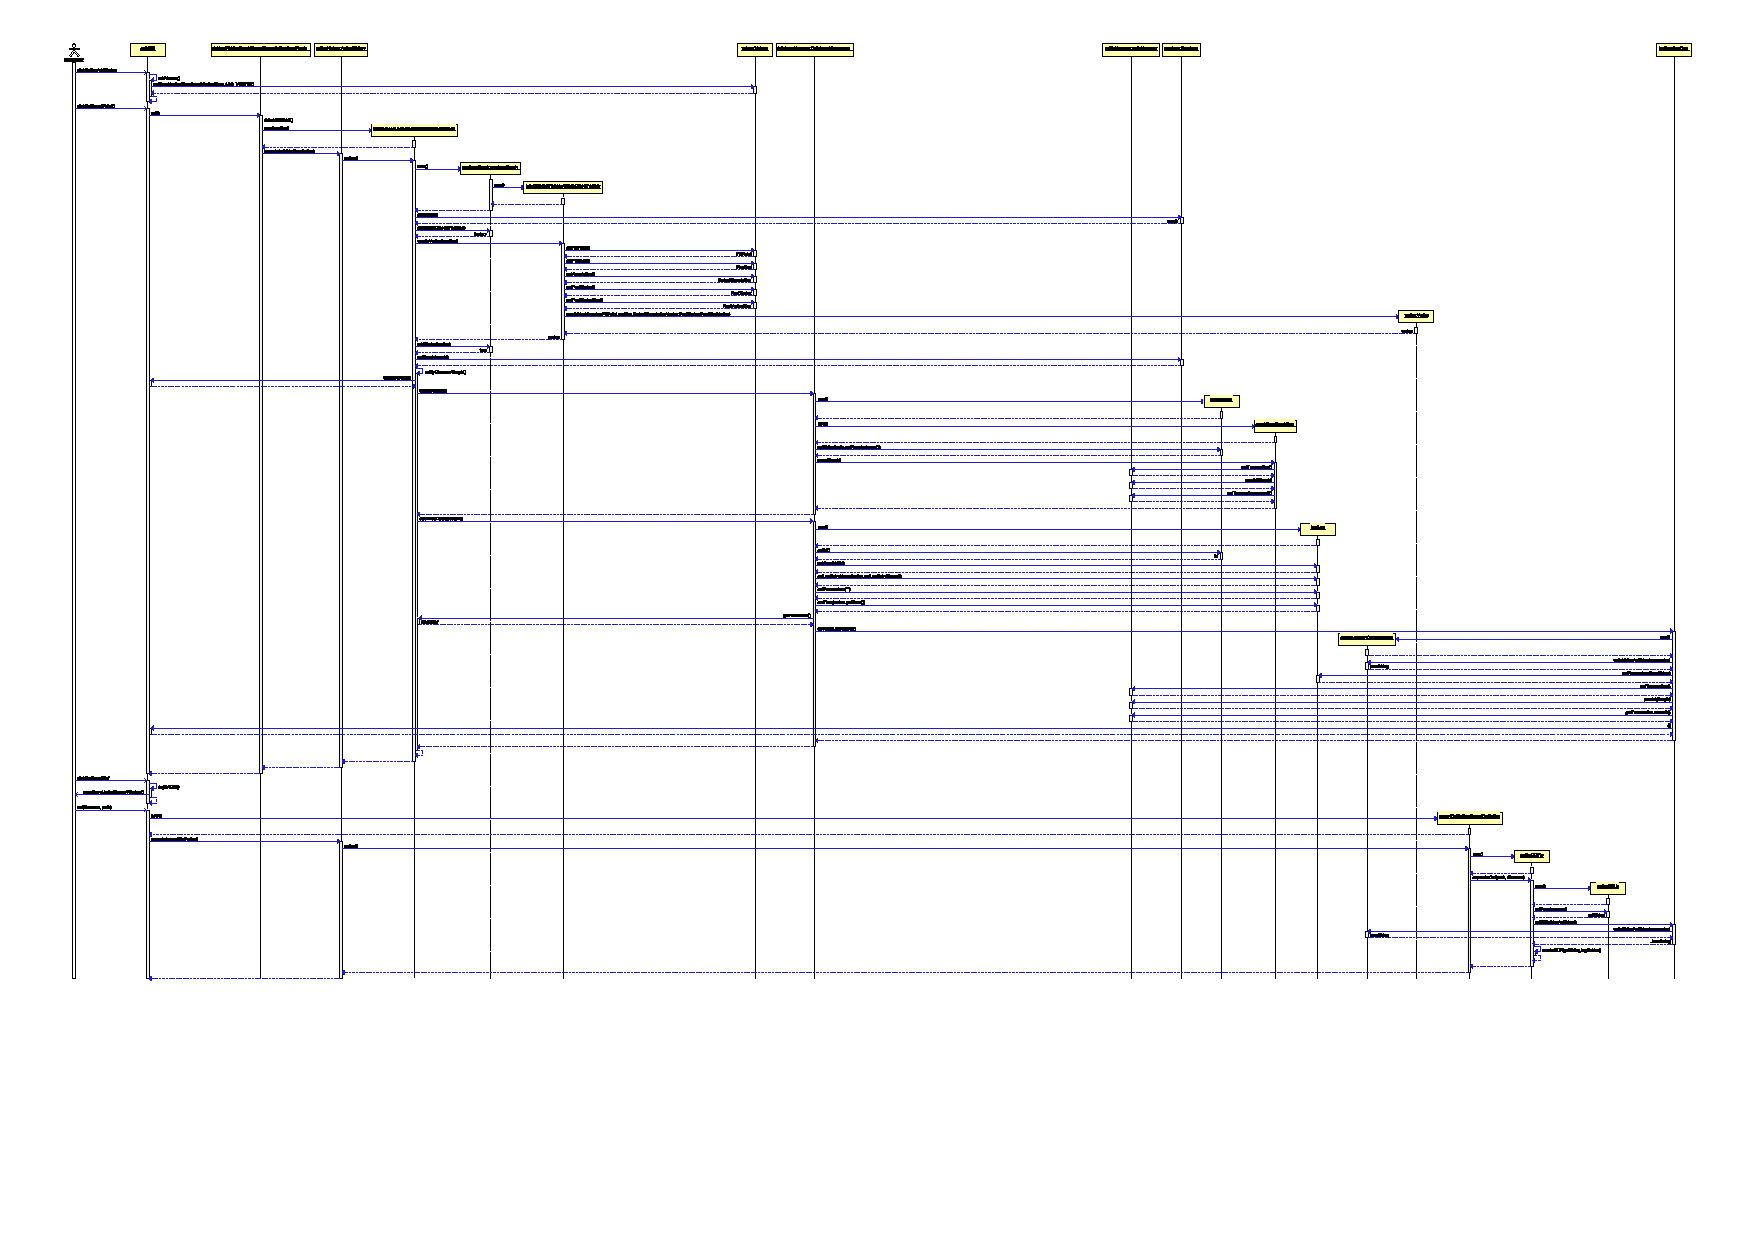
\includepdf[pages=-, landscape, scale=0.84,pagecommand={\pagestyle{fancy}}]{third.pdf}

\newpage

\subsection{Anwendungsfall: Schüler korrigiert Graph mit falschen Relationen/Symptomen.}

\begin{tabular} {|p{16cm}|}
	\hline
	\rowcolor{anw}\parbox{16cm}{\textbf{A4: Bearbeiter korrigiert Syndromansatz}} \\\hline
	\hline
	\textbf{Akteure}:  Bearbeiter
	\\\hline
	\textbf{Vorbedingungen}: Das Programm ist geöffnet. Die GXL-Datei ist erfolgreich importiert. Diese enthält genügend Sphären und Knoten, die miteinander verknüpft sind.\\ 
	\textit{Ziel}: Syndromansatz modifizieren.
	\\\hline
	\textbf{Regulärer Ablauf}:
\begin{itemize}
	\itemsep-0.5em
	\item der Bearbeiter markiert eine Kante
	\item der Bearbeiter klickt auf den Menüpunkt \textit{Reationstyp ändern} $\rightarrow$ \textit{Ungewiss}
	\item der Bearbeiter klickt auf den Menüpunkt \textit{undo}
\end{itemize}
	\\\hline
	\textbf{Varianten}: Der Bearbeiter hat eine große Auswahl an Werkzeugen z.B. \textit{Sphärenfarbe ändern} oder \textit, um den Graph zu modifizieren. 
	\\\hline
	\textbf{Nachbedingung}: Der Graph wurde durch den Bearbeiter modifiziert. Danach könnte der Bearbeiter dies nun als Vorlage speichern oder den neuen Graphen nach Kriterien auswerten.
	\\\hline
	\textbf{Fehler-/Ausnahmefälle mit deren Nachbedingung}: Der Auswerter könnte mehrere Knoten auf nicht erlaubte Positionen verschieben. Das System gibt dann eine Warnmeldung aus und untersagt die Aktion.
	\\\hline
\end{tabular}\\ \\ \\

\begin{figure}[ht]
	\centering
	%  \includegraphics[width=1\textwidth]{seqdia.jpg}
	\caption{Sequenzdiagram III}
\end{figure}

\newpage

\subsection{Anwendungsfall: Ein Lehrer exportiert einen Graphen}

\begin{tabular} {|p{16cm}|}
	\hline
	\rowcolor{anw}\parbox{16cm}{\textbf{A5: Bearbeiter exportiert einen Graphen}} \\\hline
	\hline
	\textbf{Akteure}: Bearbeiter
	\\\hline
	\textbf{Vorbedingungen}: Das Programm ist geöffnet. Die GXL-Datei ist schon importiert. Es existiert eine Sphäre und ein Knote in der Sphäre.\\ 
	\textit{Ziel}: Graphen exportieren.
	\\\hline
	\textbf{Regulärer Ablauf}:
\begin{itemize}
	\itemsep-0.5em
	\item der Bearbeiter klickt auf den Menüpunkt \textit{Datei} $\rightarrow$ \textit{exportieren als} $\rightarrow$ \textit{PDF}
	\item das System öffnet ein Pop-Up-Fenster
	\item der Bearbeiter gibt den Speicherpfad des Graphen an und klickt \textit{Ok}
\end{itemize}
	\\\hline
	\textbf{Varianten}: Zwischendurch kann der Bearbeiter den Graphen modifizieren und anschließend exportieren, sodass der Bearbeiter Exporte verschiedener Versionen hat.
	\\\hline
	\textbf{Nachbedingung}: Der Graph ist nun als PDF exportiert. Die OOF-Datei kann der Bearbeiter nun weitergeben, sodass jemand anderes den ausdrucken kann.
	\\\hline
	\textbf{Fehler-/Ausnahmefälle mit deren Nachbedingung}: Der Bearbeiter könnte einen falschen Pfad angeben $\rightarrow$ das System warnt den Bearbeiter und der Bearbeiter kann es erneut versuchen.
	\\\hline
\end{tabular}\\ \\ \\

Das folgende Sequenzdiagramm stellt den Fall dar, bei dem ein Benutzer den bestehenden Graphen als PDF exportiert. Klickt also der Benutzer auf den Button \textit{Exportieren als} $\rightarrow$ \textit{PDF}, reagiert darauf \texttt{GUI} mit einem Dialogfenster, bei dem der Nutzer einen validen Pfad eingeben und mit dem Button \textit{Exportieren} dies bestätigen muss. \\
Eine neue Action \texttt{exportPdfAction} wird erstellt und wieder durch die \texttt{ActionHistory} ausgeführt. Von Syndrom wird der \texttt{VisualisationViewer} geholt und an die Action übergeben. Mithilfe dieser Information wird eine neues Objekt von der Klasse \texttt{PDFIo} erstellt und initialisiert. Weiter im Verlauf der Action wird mithilfe der Methode \texttt{exportPDF()} ein neuer \texttt{ExportDialog} erstellt und darauf die Methode ausgeführt, die die PDF erstellt.\\ \\

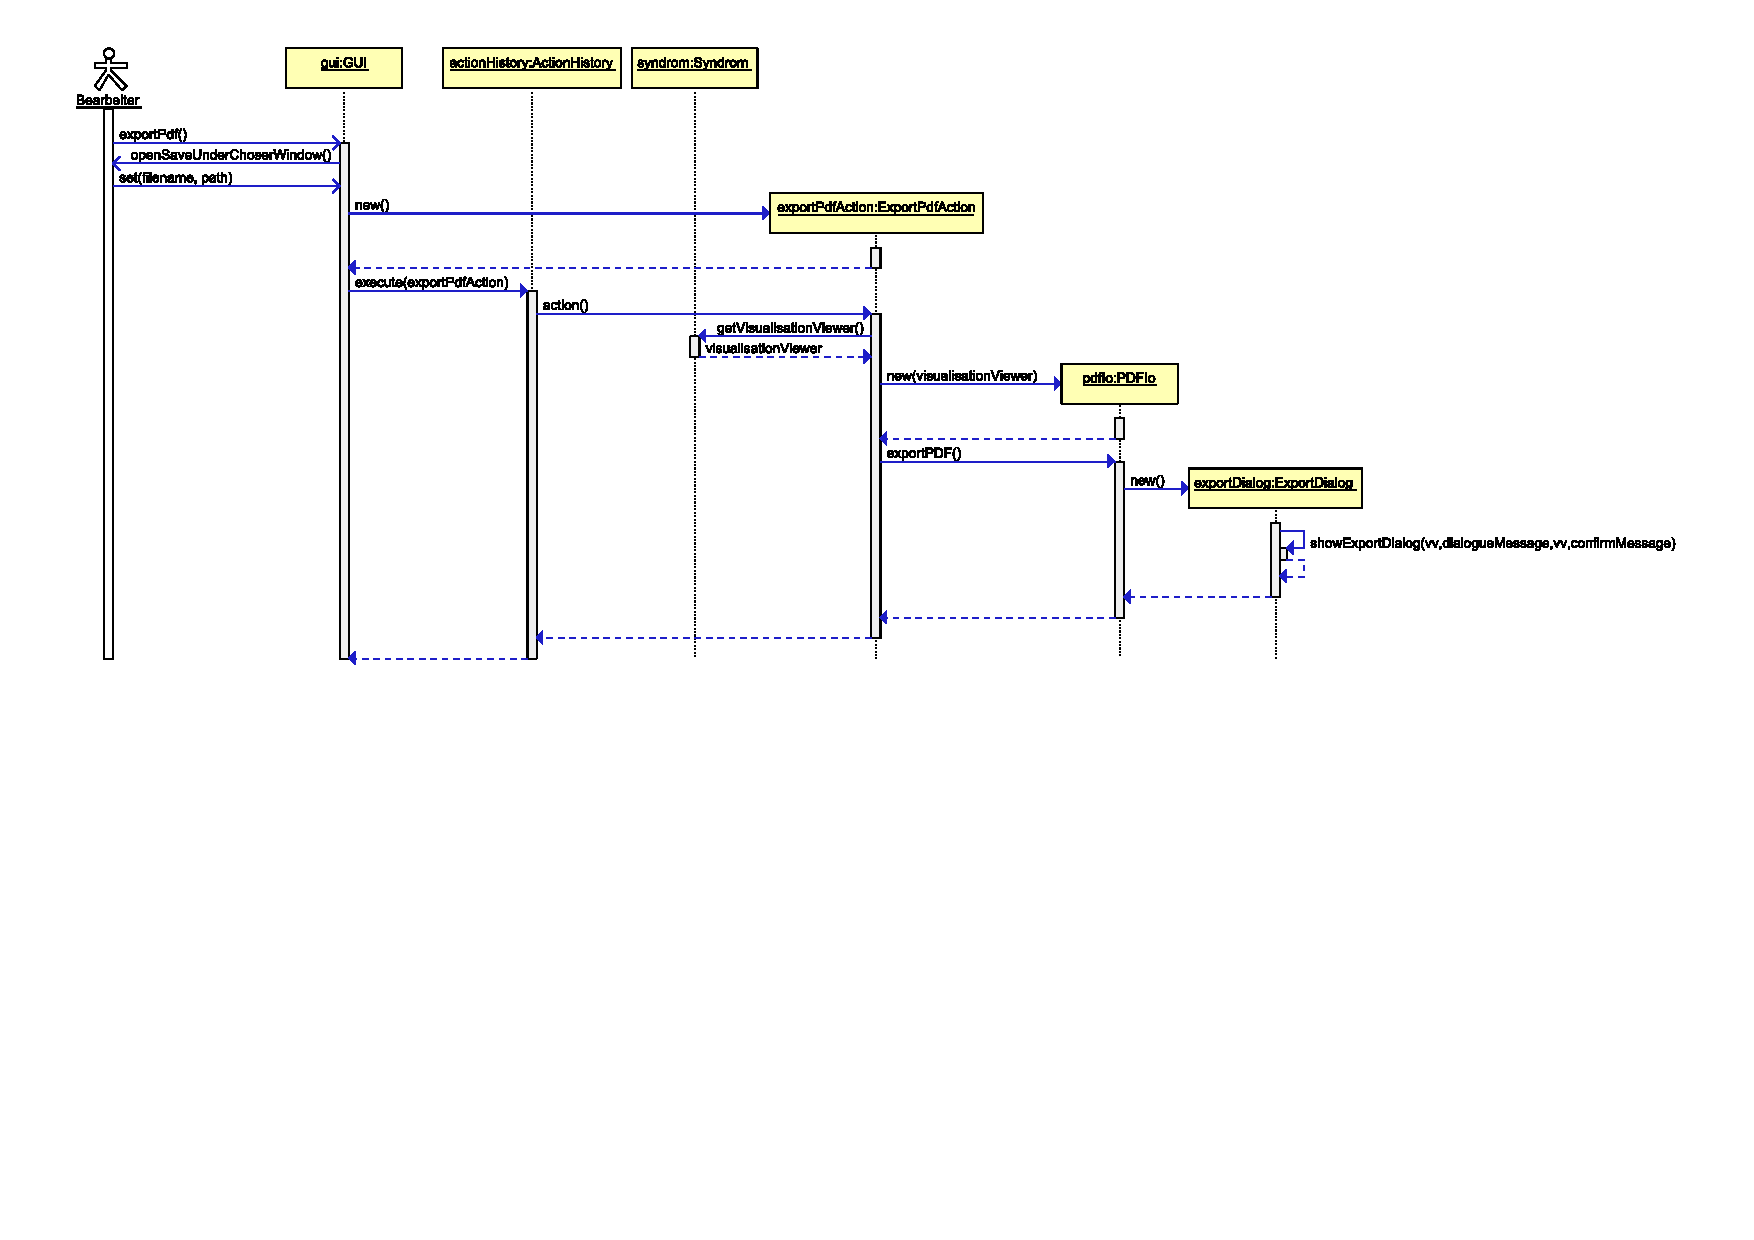
\includepdf[pages=-, landscape, scale=0.84,pagecommand={\pagestyle{fancy}}]{fifth.pdf}


\newpage
\section{Evolution}
\label{sec:evolution}
\emph{Autoren: Bastian Rexhäuser, Anthony Mendil}\\\\
In diesem Kapitel wollen wir beschreiben wie sich ändernde Anforderungen auf unsere Architektur auswirken würden. Dabei gehen wir zunächst auf die Einflussfaktoren ein, deren Veränderlichkeit im Rahmen der globalen Analyse als eher hoch oder gar sehr hoch eingeschätzt wurde. Hierbei betrachten wir lediglich die, die Einfluss auf die Architektur haben. Allerdings haben wir keinen Einflussfaktor als sehr veränderlich eingestuft, sodass wir lediglich jene mit einer eher hohen Veränderlichkeit thematisieren werden. Bei den entsprechenden Einflussfaktoren werden wir beschreiben, welchen Einfluss eine potentielle Änderung des Einflussfaktors (beziehungsweise der Anforderung, die durch diesen Einflussfaktor repräsentiert werden) auf unsere Architektur hätte. Im Anschluss daran werden wir auf die Anforderungen aus dem Chinese Menue eingehen, deren Umsetzung in unserer Architektur aktuell nicht vorgesehen ist. Hier werden wir erklären wie sich die nachträgliche Umsetzung dieser Anforderungen unsere Architektur beeinflussen würde. \\ 
 
Für die Filterung von Knoten und Kanten (\hyperlink{ss}{Filter von Knoten und Kanten}) könnten weitere Filteroptionen benötigt werden. Eine Erweiterung wäre zum Beispiel, dass der Benutzer als zusätzliche Filteroption die Knoten, Kanten und Sphären ausblenden kann, die in einem bestimmten Zeitraum hinzugefügt wurden. Hierfür könnte man in der GUI  ein Textfeld hinzufügen. Wird eine Zeitspanne (z.B 11:23-13:04) eingegeben, werden nur Elemente angezeigt, die in diesem Zeitraum hinzugefügt wurden. Es ist jedoch auch möglich mit relativen Zeiten zu arbeiten. Wird -00:10 eingegeben, werden nur Elemente angezeigt, die höchstens 10 Minuten vor dem letzten hinzugefügten Element hinzugefügt wurden und wird +00:10 eingegeben, werden die angezeigt, die höchstens 10 Minuten nach dem ersten hinzugefügten Element hinzugefügt wurden. Dies könnten wir Realisieren, indem wir uns aus den Log-Einträgen die Einträge heraussuchen, die hinzufügende Aktionen beschreiben und deren Erstellungszeitpunkt sich im angegebenen Zeitraum befindet. Dann müssen die Identifikationsnummern der Graph-Elemente extrahiert und ausgeblendet werden. An dieser Stelle ist zu erwähnen, dass es auf diese Weise nicht möglich ist, Elemente die bereits in der Vorlage hinzugefügt wurden, zu filtern, da im Ersteller-Modus keine Log-Einträge erstellt werden. Hierfür müsste im Package \texttt{actions.analyse} die Klasse \texttt{FilterGraphAction} angepasst werden und im Package \texttt{graph.algorithmen.predicate} eine Klasse \texttt{ElementsCreatedInTimePredicate} hinzugefügt werden. \\

Wie in der globalen Analyse zu sehen weist der Einflussfaktor \hyperlink{z}{Funktionsmodi (Ersteller, Bearbeiter, Auswerter)} eine eher hohe Veränderlichkeit auf. Eine mögliche Änderung dieses Faktors wäre beispielsweise das Hinzukommen einer Rolle, mit der es möglich wäre, eine Vorlage auszuwerten oder einen erstellten Graphen zu kommentieren.
Die Auswertung einer Vorlage könnte in einer statistischen Auswertung des Anteils der Knoten, Sphären und Kanten in einer Vorlage bestehen, die später im \hyperlink{„Diagramm bearbeiten“-Modus}{„Diagramm bearbeiten“-Modus} vollständig beziehungsweise nur eingeschränkt (nur Farbe, nur Beschriftung) bearbeitet werden können. Im folgender ist in diesem Fall vom Vorlage-Analyse-Modus die Rede.
Das Kommentieren eines erstellten Graphen ist wie folgt zu verstehen. Ein Graph kann geöffnet werden, wobei keine Eigenschaften mehr verändert werden können. Man kann allerdings die einzelnen Sphären, Knoten und Kanten anklicken (auch mehrere gleichzeitig, wenn sich das Kommentar auf mehrere Graph-Elemente bezieht) und einen Hinweis zu diesen schreiben. Dieser Hinweise könnten dann nach Speichern / Exportieren des Graphen auch auf einem anderen Rechner gelesen werden. Voraussetzung ist die Aktivierung desselben Modus (wobei die Hinweise weiterhin verändert und auch wieder gelöscht werden könnten. Dieser Modus wird im Folgenden als Diagramm-Kommentieren-Modus bezeichnet.
Eine solche Änderung (das Hinzukommen von neuen Funktionsmodi mit neuen Funktionen) würde sich auf die im Package \texttt{graph.graph} befindliche Klasse \texttt{FunctionMode} sowie auf die Klasse \texttt{SwitchModiEditorAction} im Package \texttt{actions.io}. Über letztgenannte würde dann auch eine Änderung der Benutzeroberfläche ausgelöst werden. Die entsprechende Benutzeroberfläche würde Änderungen am \texttt{gui}-Package erforderlich machen, um eine den Anforderungen des neuen Funktionsmodus entsprechende Benutzeroberfläche bereitstellen zu können.
Für die Funktionalitäten des Vorlage-Analyse-Modus müsste außerdem eine Klasse (oder mehrere Klassen) im Package \texttt{actions.analyse} hinzugefügt werden, die eine entsprechende Filterung der Knoten, Kanten und Sphären vornehmen und durch Rechenoperationen den jeweiligen Anteil (entsprechend der Bearbeitungsmöglichkeiten) bestimmen würde.
Um die Funktionen des Diagramm-Kommentieren-Modus bereitzustellen, müsste unser System neben den oben erwähnten auch noch an folgenden Stellen angepasst werden: Die Klassen \texttt{Edge}, \texttt{Vertex} und \texttt{Sphere} im \texttt{graph.graph}-Package um ein Attribut zum, Soeichern des Kommentares erweitert werden. Dazu müsste man im \texttt{actions}-Package ein Package \texttt{comment} hinzufügen, in dem Klassen zum Hinzufügen, Editieren und Löschen von Kommentaren zu Sphären, Knoten und Kanten enthalten wären. \\
 
Es ließen sich zusätzlich Wegpunkte (\texttt{O«Wegpunkte»}) mit dem Framework JGraph realisieren. Dazu müssten wir den Java-spezifischen Teil (JrapX) dieses Frameworks in unser System integrieren. Da man Wegpunkte innerhalb dieses Frameworks auf Edge-Objekten hinzufügt, müssten wir in unserem System statt unserer \texttt{Edge}-Klasse diejenige von JGraphX verwenden. Da diese ihrerseits allerdings nicht alle von uns benötigten Informationen (in Form von Attributen) enthält, müssten wir weiterhin eine eigene \texttt{Edge}-Klasse in unserem System vorhalten. Diese müsste allerdings anders als bis jetzt die Edge-Klasse von JGraphX erweitern. Diese alternative beziehungsweise neue \texttt{Edge}-Klasse würde dann überall dort verwendet, wo aktuell unsere jetzige \texttt{Edge}-Klasse angewandt wird. Zu diesen Änderungen müsste auch im \texttt{actions}-Package je eine Aktion zum Hinzufügen beziehungsweise Entfernen von Wegpunkten hinzugefügt werden. \\

Des weiteren wäre die Realisierung von Kantenbündelung (\texttt{O«Kantenbündelung»}) möglich, indem wir im Package \texttt{actions.visualization.renderers} die Klasse \texttt{EdgeRenderer} mithilfe eines selbst geschriebenen Algorithmus so anpassen, dass die Kanten entsprechend gerendert werden. Abgesehen davon hätte dies keine weiteren Auswirkungen auf die Architektur.  \\

Um eine mobile Version (\texttt{O«Mobil»}) des Programms zu unterstützen müsste eine neue Applikation erstellt werden, wobei einige umfangreiche Anpassungen vorgenommen werden müssten. Dies betrifft in erster Linie die Benutzeroberfläche (Package: gui), da diese von Grund auf neu zu gestalten ist, um auf mobilen Geräten nutzerfreundlich bedienbar zu sein. Hierbei unterstützen Android sowie IOS die Umsetzung der Benutzeroberfläche mittels JavaFX. Die Nutzung von der H2 Datenbank ist lediglich unter Android möglich. Für IOS bietet sich unter anderem ein sqlite-Datenbank an. Übrige Komponenten könnten größtenteils übernommen werden. 

\end{document}


%%% Local Variables:
%%% mode: latex
%%% mode: reftex
%%% mode: flyspell
%%% ispell-local-dictionary: "de_DE"
%%% TeX-master: t
%%% End:
